%************************************************
\chapter{Research and Development Testbed For Future Liquid Xenon TPCs}

\label{ch:testbed} % $\mathbb{ZNR}$
%************************************************

\begin{flushright}{\slshape    
  All systems go, are you sure? } \\ \medskip
    --- {Peter Schilling \textit{Major Tom, 1969}}
\end{flushright}


A small test bed was built at Lawrence Berkeley National Laboratory to study various detector effects facing large \ac{LXe} \ac{TPC}s. The test bed was built and instrumented over the course of about two years, from 2015 through 2016. This chapter describes some of the details of that instrumentation.

\section{Test Bed Apparatus Overview}

\begin{figure}[htbp]
\begin{center}
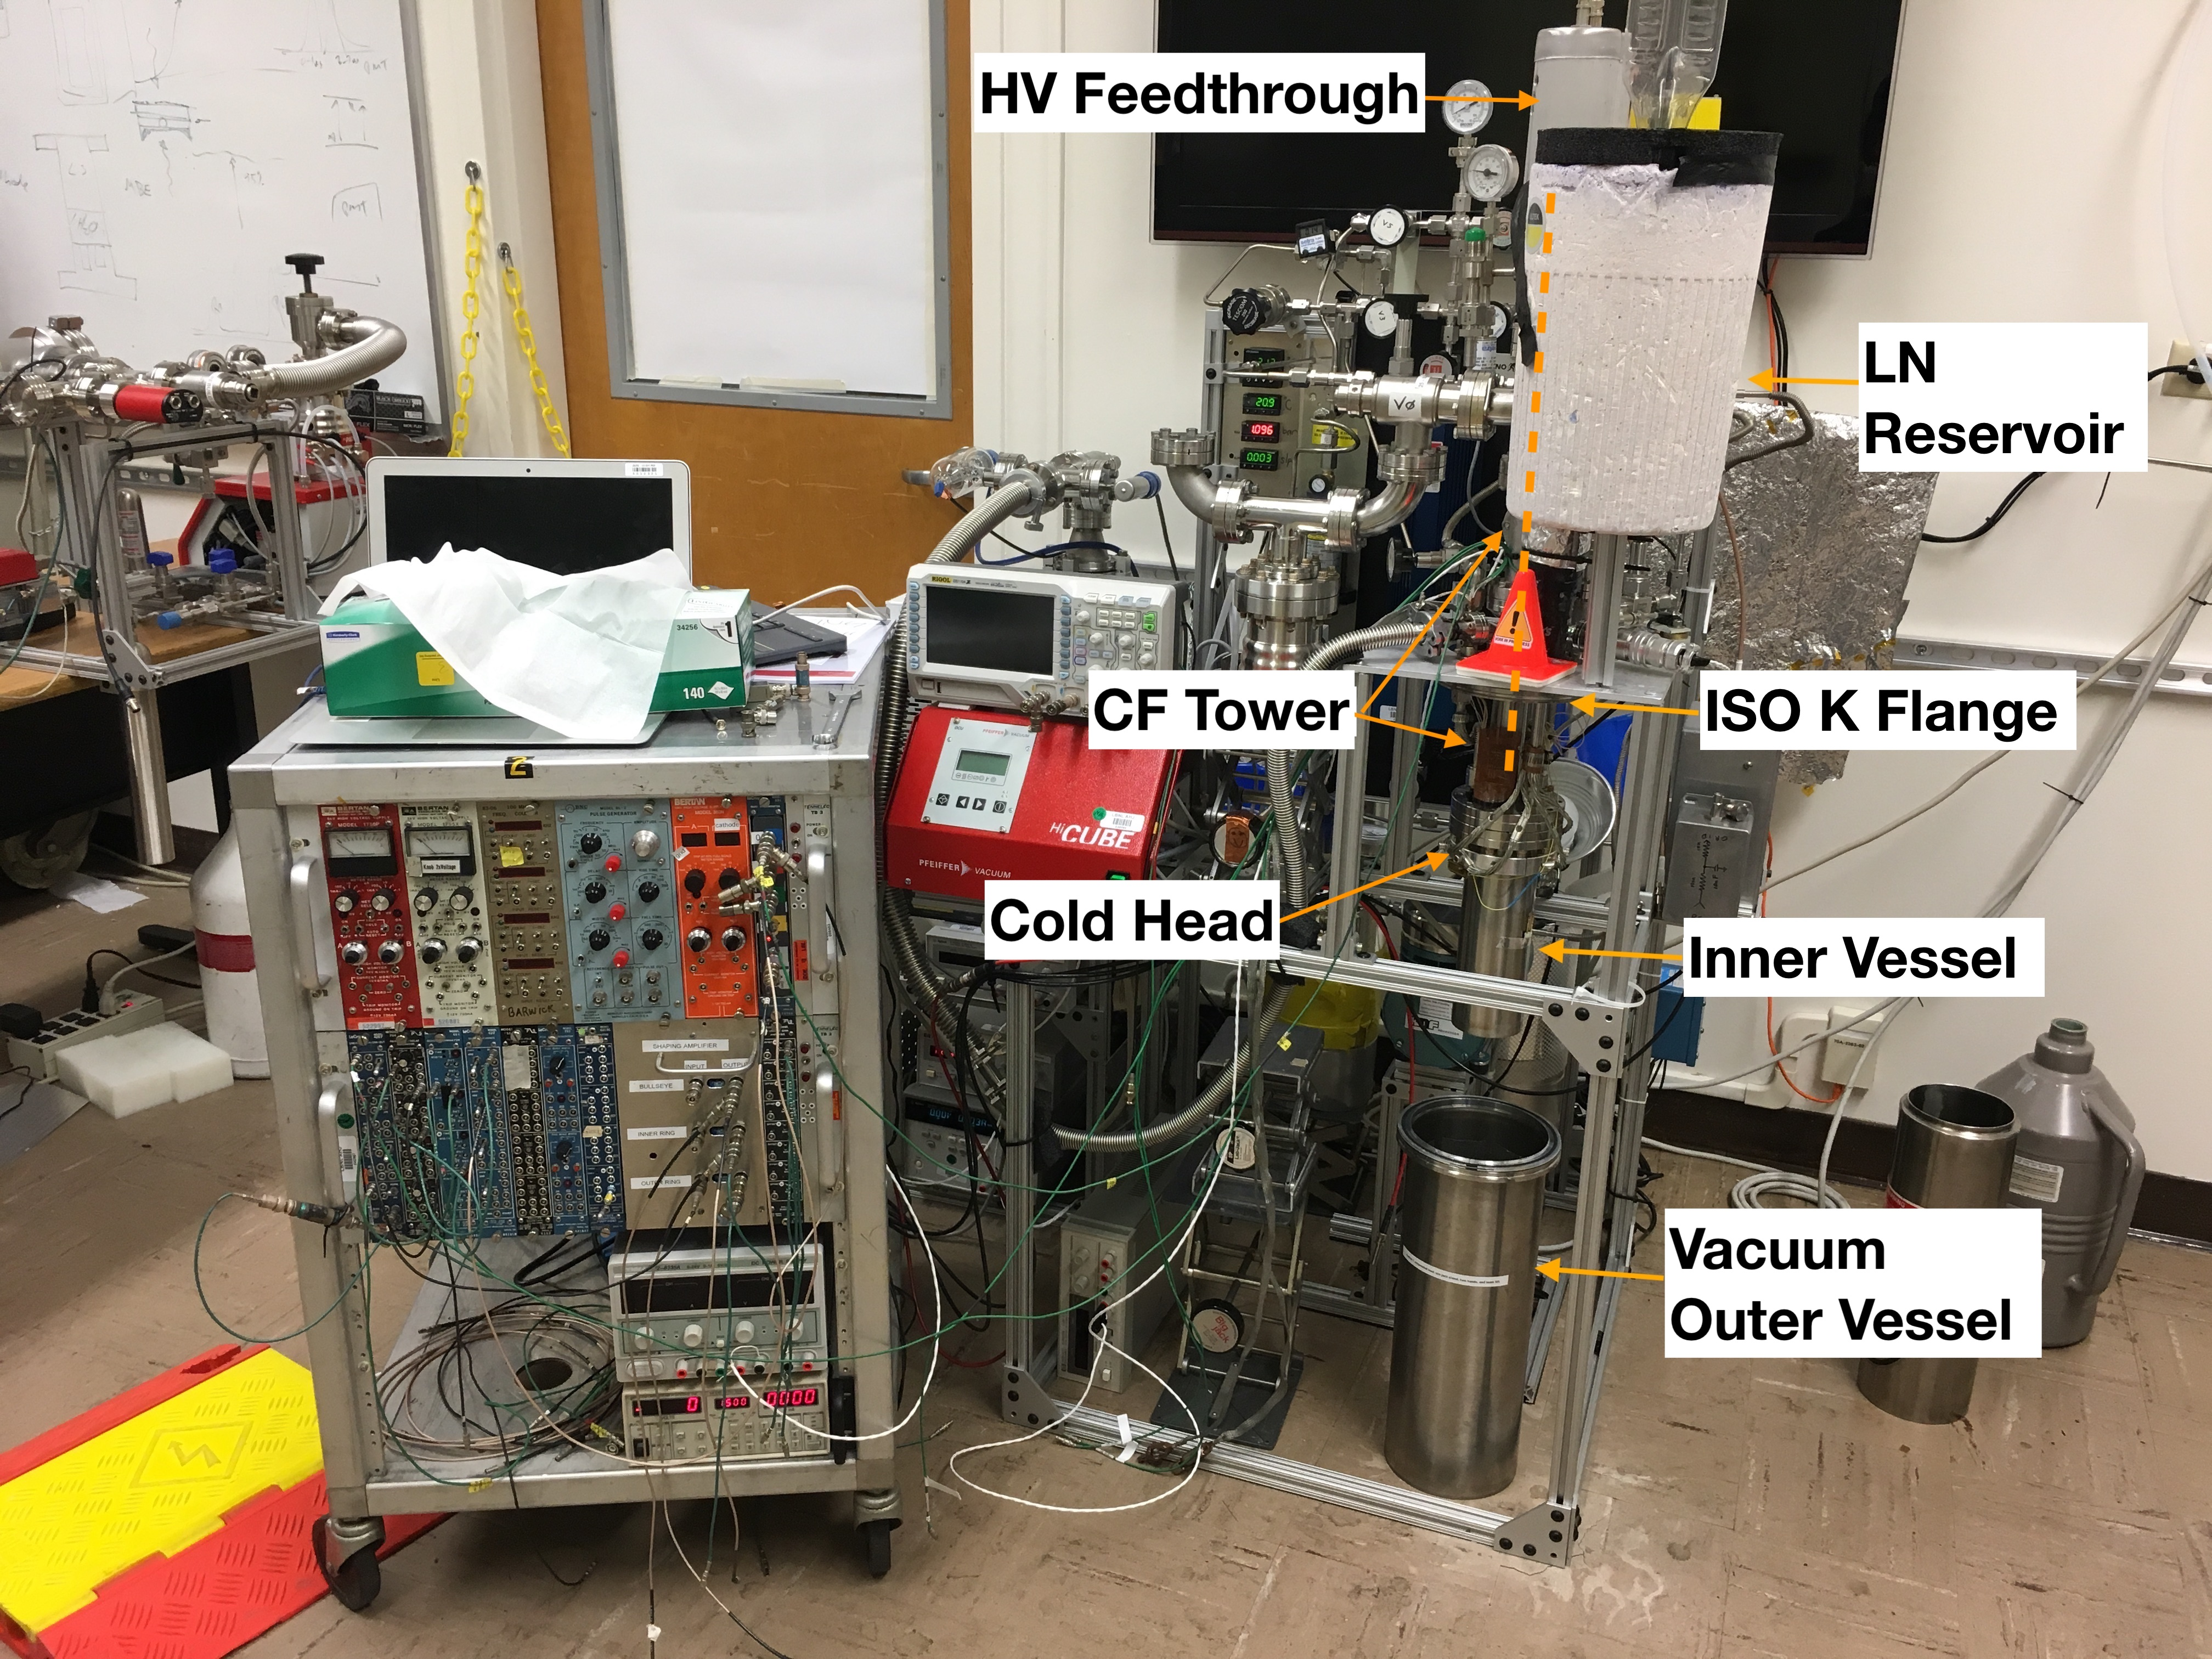
\includegraphics[width=\textwidth]{figures/testbed/apparatus.jpg}
\caption{Large scale view of the experimental apparatus showing key parts. The \acs{CF} tower extent is indicated with a dotted line; this whole tower is also part of the inner xenon space.}
\label{fig:apparatus}
\end{center}
\end{figure}

A large-scale overview of the testbed is shown in Figure~\ref{fig:apparatus}, and a diagram of the inner experimental vessel is shown in Figure~\ref{fig:internals}. The experimental apparatus consisted of an inner vessel, a vacuum outer vessel, and a xenon circulation system. The inner vessel was a \ac{SS} canister, topped with a 2.75~in Conflat-adaptable tower that allowed space for instrumentation cabling and \ac{HV} feedthroughs. The inner vessel was offset below a 7.09~in ISO K flange, which held the (removable) vacuum outer vessel in place. Several Mini-CF ports were welded to the ISO K flange for instrumentation cabling. A \ac{LN} reservoir was thermally connected to the cold-head. A half-inch pipe opened into the bottom of the reservoir, which was offset above the ISO-K flange; this allowed \ac{LN} to flow into the pipe. The bottom of the pipe was connected to the cold-head via braided copper wire. A Swagelock vacuum fitting sealed the lower-half of the pipe into the outer vacuum space.

The inner vessel contained the \ac{TPC}. A \ac{PTFE} housing cylinder fastened a \ac{PMT} in place. Above the \ac{PTFE} housing, a series of interlocking \ac{PTFE} rings held strung wire grids and a segmented anode in place. During data taking, the entire \ac{PMT} and housing were immersed in \ac{LXe}. The liquid level was chosen depending on the experiment being performed, and was approximated by the S2 width. In some cases, the \ac{TPC} was ``overfilled'' by allowing the liquid level to rise above the anode. The segmented anode was instrumented with charge amplifiers for direct charge readout. When the \ac{TPC} was overfilled, the charge amplifiers detected the ionization electrons directly from the liquid. During typical dual phase \ac{TPC} operation, the charge amplifiers provided a secondary measurement of the ionization electrons in addition to S2. Two typical arrangements of the inner vessel are shown in Figure~\ref{fig:internals}.

\begin{figure}[htbp]
\begin{center}
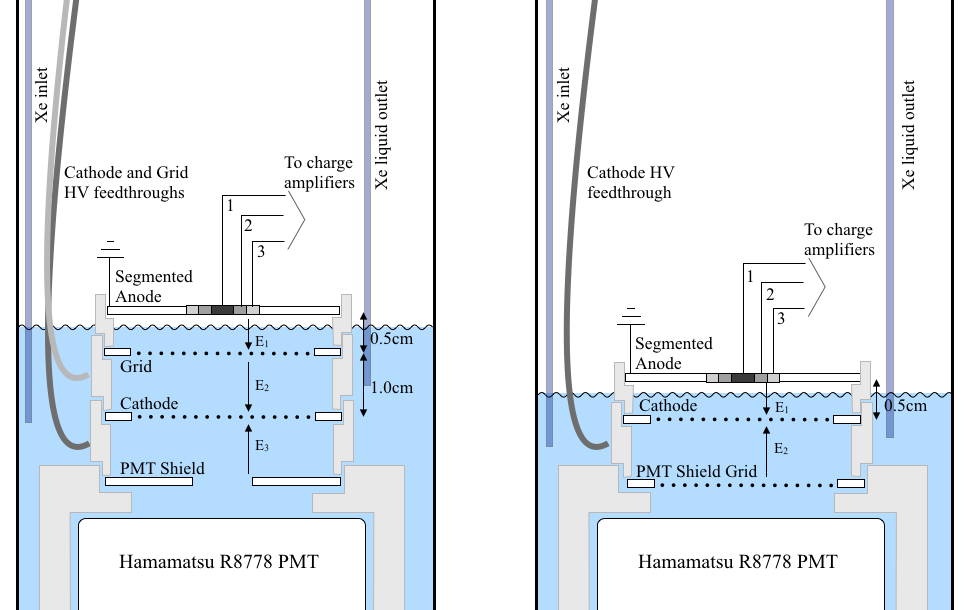
\includegraphics[width=\textwidth]{figures/testbed/internals_1and2.png}
%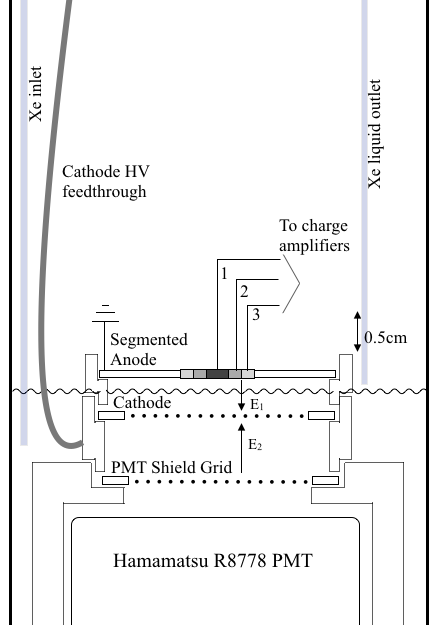
\includegraphics[width=\halffig]{figures/testbed/internals1.png}
%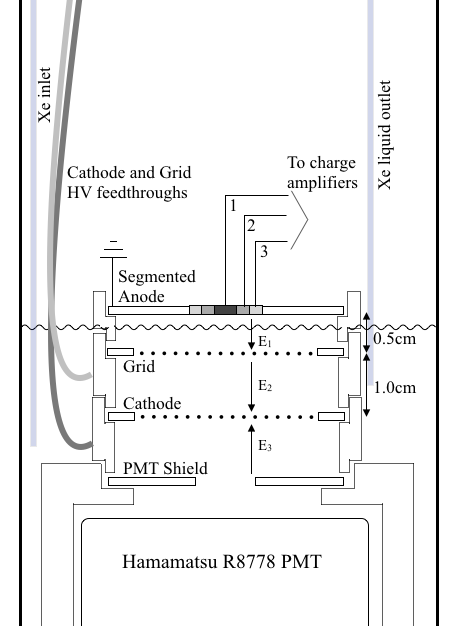
\includegraphics[width=\halffig]{figures/testbed/internals2.png}
\caption{Diagrams of two often used internal arrangements. The configuration (left) has both a drift and extraction region. The configuration (right) is ``extraction region only''. The blue region with the wavy line indicates the liquid level. }
\label{fig:internals}
\end{center}
\end{figure}


\section{Circulation System}
The xenon circulation system in shown in Figure~\ref{fig:circ}. A stainless steel capillary extending into the liquid drew xenon from the inner vessel during operation to be purified. Purified xenon that was returned to the vessel was directed into the liquid via a \ac{PTFE} tube so it could condense quickly. A gas purge from a \ac{CF} tower above the inner vessel could be opened to continually renew the gas column. 

\begin{figure}[htbp]
\begin{center}
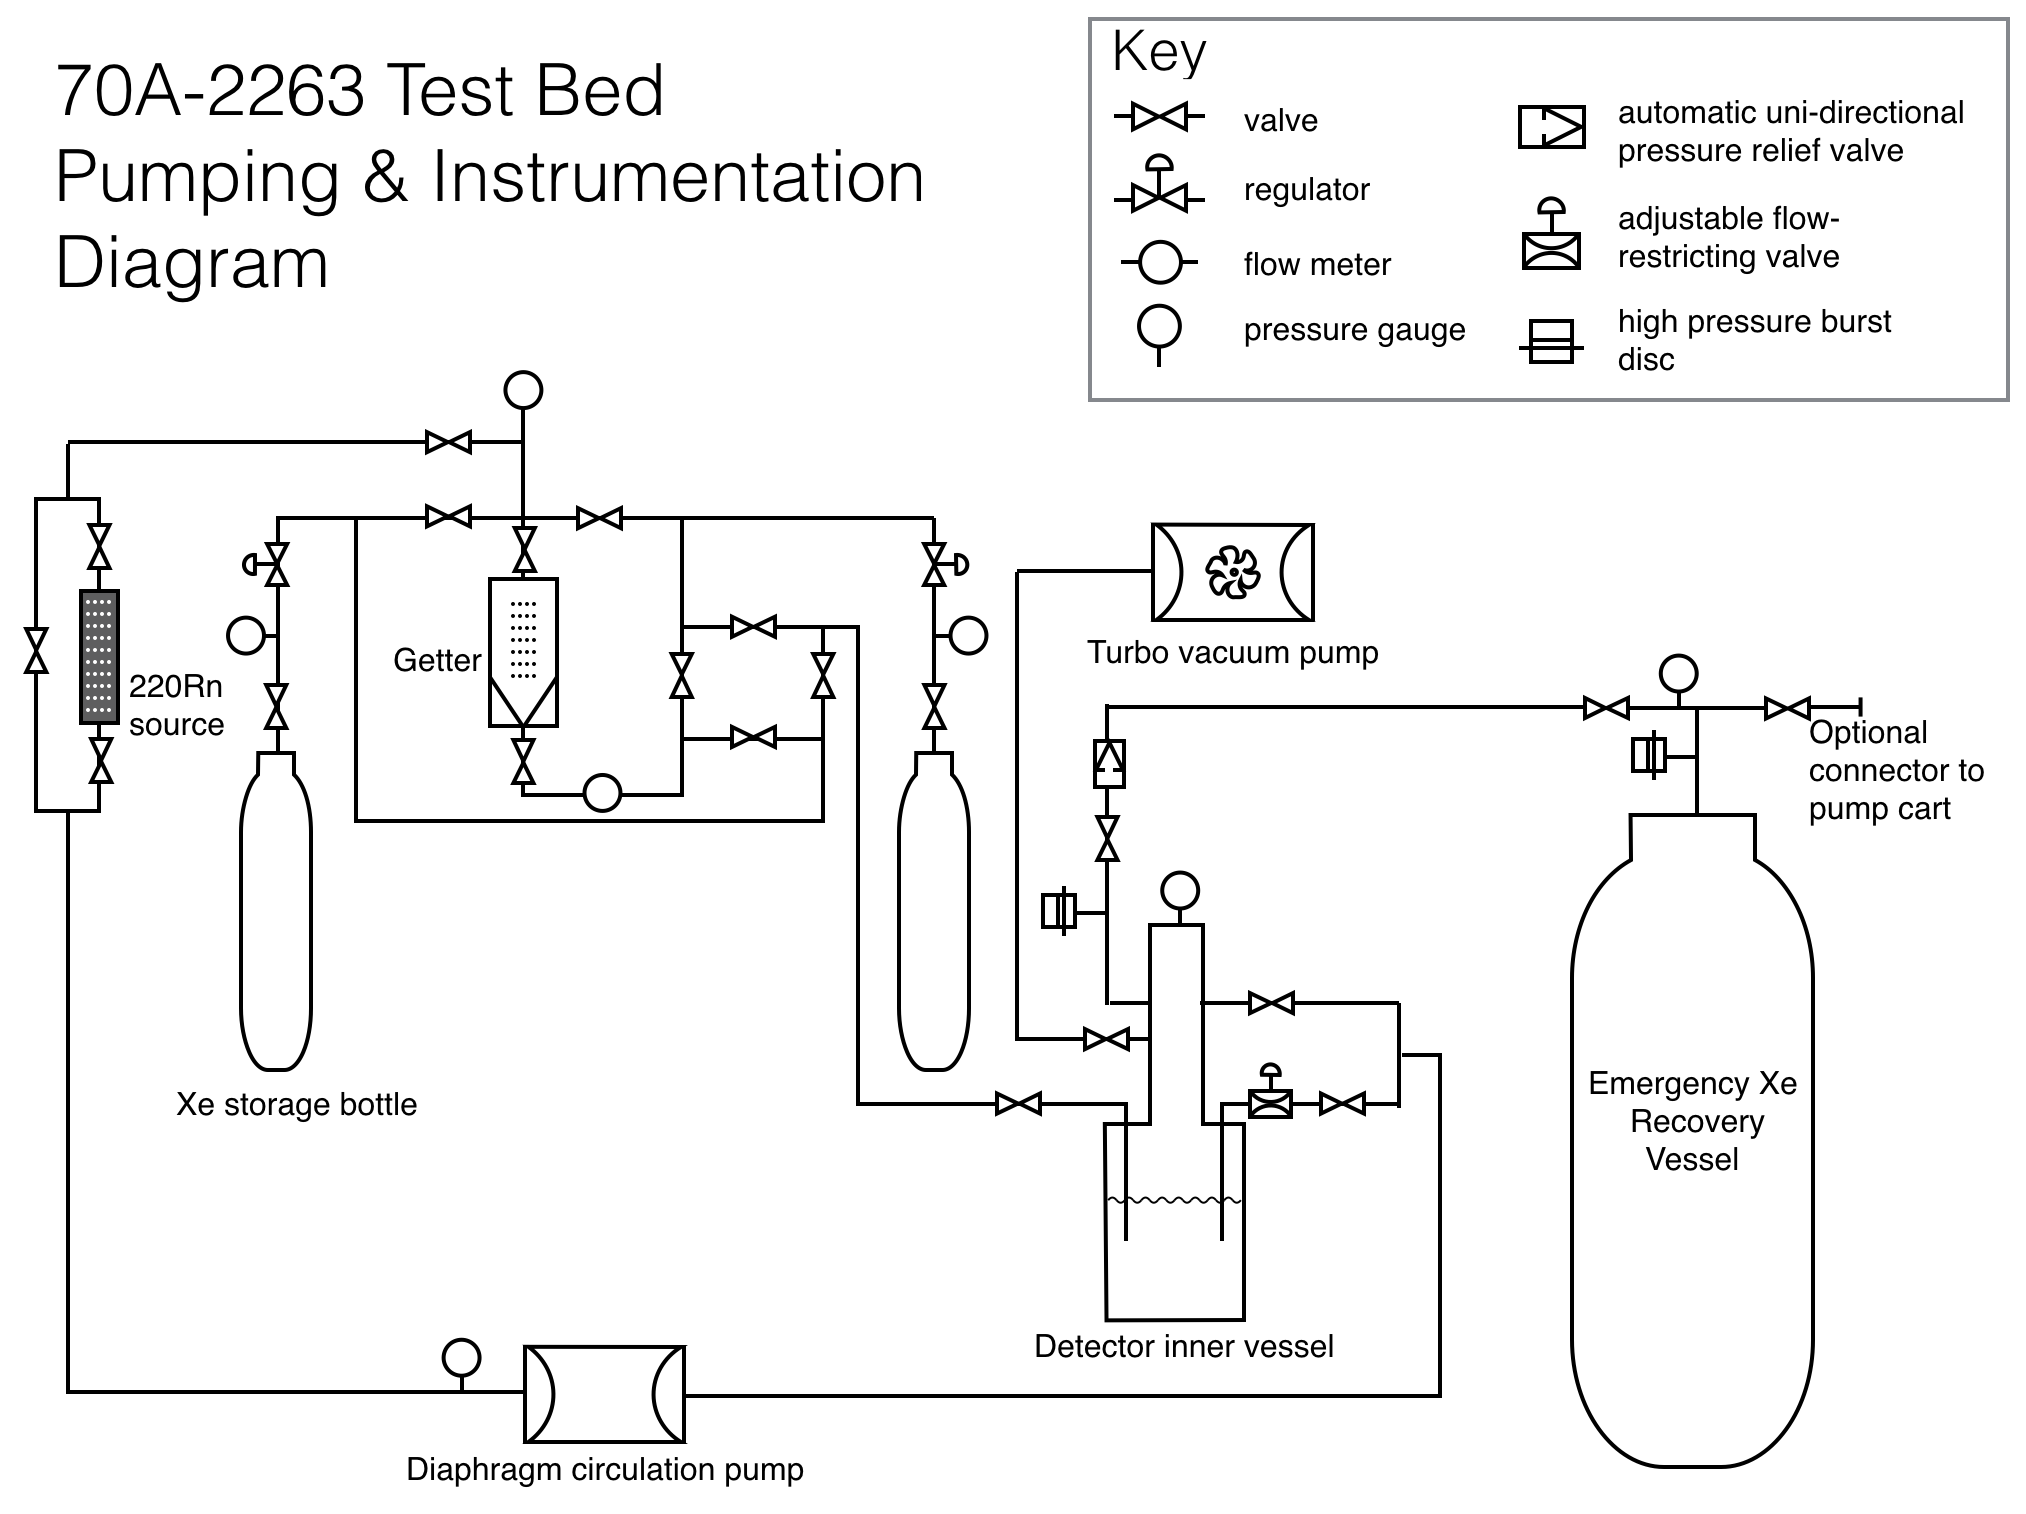
\includegraphics[width=\textwidth]{figures/testbed/full_pid.png}
\caption{Pumping and instrumentation diagram of the test bed. Special symbols are labelled in the diagram, see key for other symbols. For readability, all gauges are not shown.}
\label{fig:circ}
\end{center}
\end{figure}


\section{Slow Control}
The slow control for the test bed consists of a few monitoring variables such as temperature and pressure and a voltage supply that switches resistive heaters on/off. The inner experimental vessel was instrumented with two platinum \ac{RTD}s to monitor temperature and a capacitance manometer to monitor pressure. A flow meter in the circulation line determined the flow rate of xenon as it passed through the getter and returned to the inner vessel. These four variables were read using Omega i-series digital panel meters to provide a real-time display; two points of calibration were provided to the digital panel meters to translate voltage to human-readable pressure, temperature, etc. In addition, two 25~$\Omega$ resistors are mounted, in parallel, on the cold-head. Supplying voltage to these resistors raised the temperature of the cold-head and decreased the cooling power delivered by the liquid nitrogen bath; the voltage supplied to the heaters was also recorded, but not shown with digital panel meters. The voltages for the monitoring variables and the heater voltages were fed into a USB Device from Measurement Computing, which interfaces with a computer. A slow control script on a lab computer recorded the monitoring variables and heater voltages. The script also determined if power should be supplied to the heaters and if text message and e-mail alarms should be sent for a variable out of expected range. A basic schematic of the slow control is shown in Figure~\ref{fig:sc}.

\begin{figure}[htbp]
\begin{center}
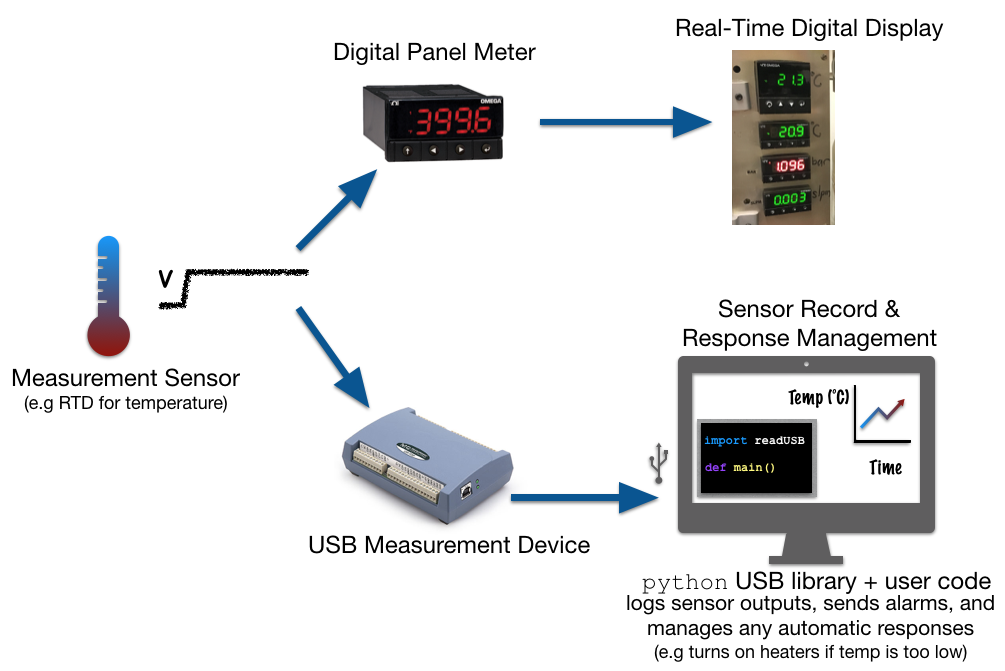
\includegraphics[width=\textwidth]{figures/testbed/slow_control.png}
\caption{A diagram showing components of the slow control.}
\label{fig:sc}
\end{center}
\end{figure}


\section{PMT}
The test bed was instrumented with a Hammamatsu R8778 \ac{PMT}, the same model of \ac{PMT} used in \ac{LUX}. A \ac{LUX} \ac{PMT} base was used and an \ac{LZ} \ac{PMT} base was tested. The radon daughters study presented in Chapter~\ref{ch:radon} exclusively used the \ac{LUX} \ac{PMT} base; the electron trains studies presented in Chapter~\ref{ch:etrains} first used the \ac{LUX} base, and later used the \ac{LZ} base. Various shaping amplifiers were used when digitizing the \ac{PMT} over the course of these studies because the 8~ns sampling interval of the data acquisition was subject to aliasing the fast-rising alpha S1 signals.



\section{Charge Amplifiers}
The \ac{TPC} diagram in Figure~\ref{fig:internals} includes a segmented anode, the largest segment of which is held at ground. The anode is pictured in Figure~\ref{fig:anode} and relevant dimensions are included in Table~\ref{T:anode_segs}.

\begin{figure}[htbp]
\begin{center}
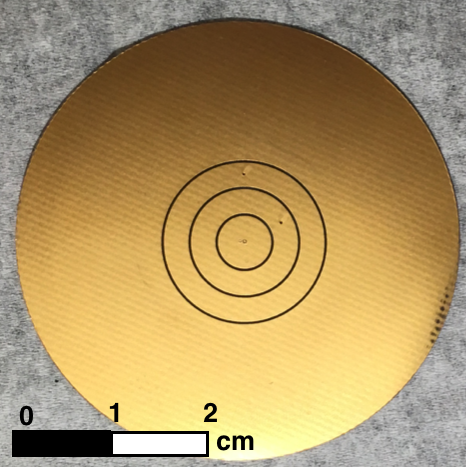
\includegraphics[width=\halffig]{figures/testbed/anode.png}
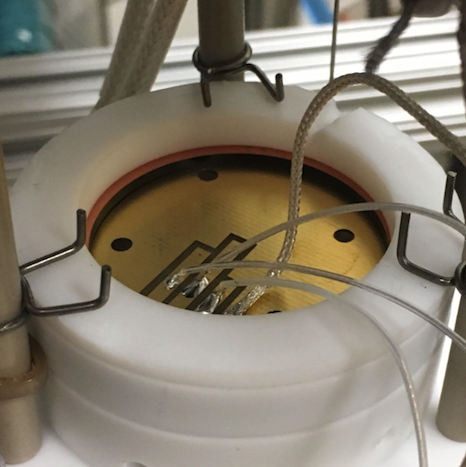
\includegraphics[width=\halffig]{figures/testbed/anode2.png}
\caption{(left) Segmented anode showing the xenon-facing anode segments. The innermost segment is referred to as the ``bullseye'', the next is called the ``inner ring'' and the last is called the ``outer ring''. The largest segment on the anode was not instrumented with charge amplifiers and was held at ground. (right) The wires on the top of the anode which lead to the charge amplifiers.}
\label{fig:anode}
\end{center}
\end{figure}

\begin{table}[ht]
\centering
\begin{tabular}{rcccc}
\hline
%& \multicolumn{3}{c}{\bf Datasets}\\[-5pt]
 Anode Segments & 1 & 2 & 3 & Full \\
\hline
Radius (mm) & 3  & 6 & 9 & 24 \\
Cumulative Area (mm$^{2}$) & 28 &  113 & 255 & 1810 \\
\end{tabular}
\caption{Dimensions of the of the anode segments. 1 refers to the inner-most segment or ``bullseye'', 2 refers to the inner ring, 3 to the outer ring and full to the entire anode, which includes inactive area that is not instrumented with charge amplifiers.}
\label{T:anode_segs}
\end{table}

The segmented anode was instrumented with three CR-110 charge amplifiers from Cremat (Figure~\ref{fig:cr110}). The raw charge amplifier signals were each fed into a CR-160-R7 shaper evaluation board, also from Cremat. The evaluation board houses two more modules: one CR-200-X shaping amplifier and one CR-110 baseline restorer. The CR-200-X shaping amplifier is an X-$\mu$s gaussian shaping amplifier; it was determined that 1~$\mu$s was most appropriate for the test bed signals, based on the size of the gas gap and the expected event rat. 

\begin{figure}[htbp]
\begin{center}
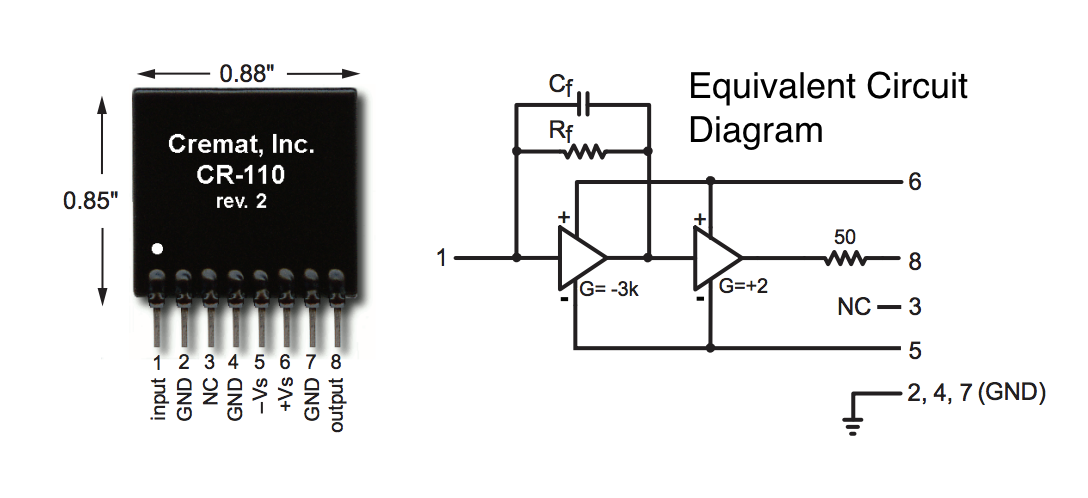
\includegraphics[width=4in]{figures/testbed/cr110.png}
\caption{A picture of the CR-110 charge amplifier from the manufacturer's data sheet, shown with an equivalent circuit diagram.}
\label{fig:cr110}
\end{center}
\end{figure}

The shaper evaluation board produced gaussian pulses from raw charge signals as shown in Figure~\ref{fig:shaper}.

\begin{figure}[htbp]
\begin{center}
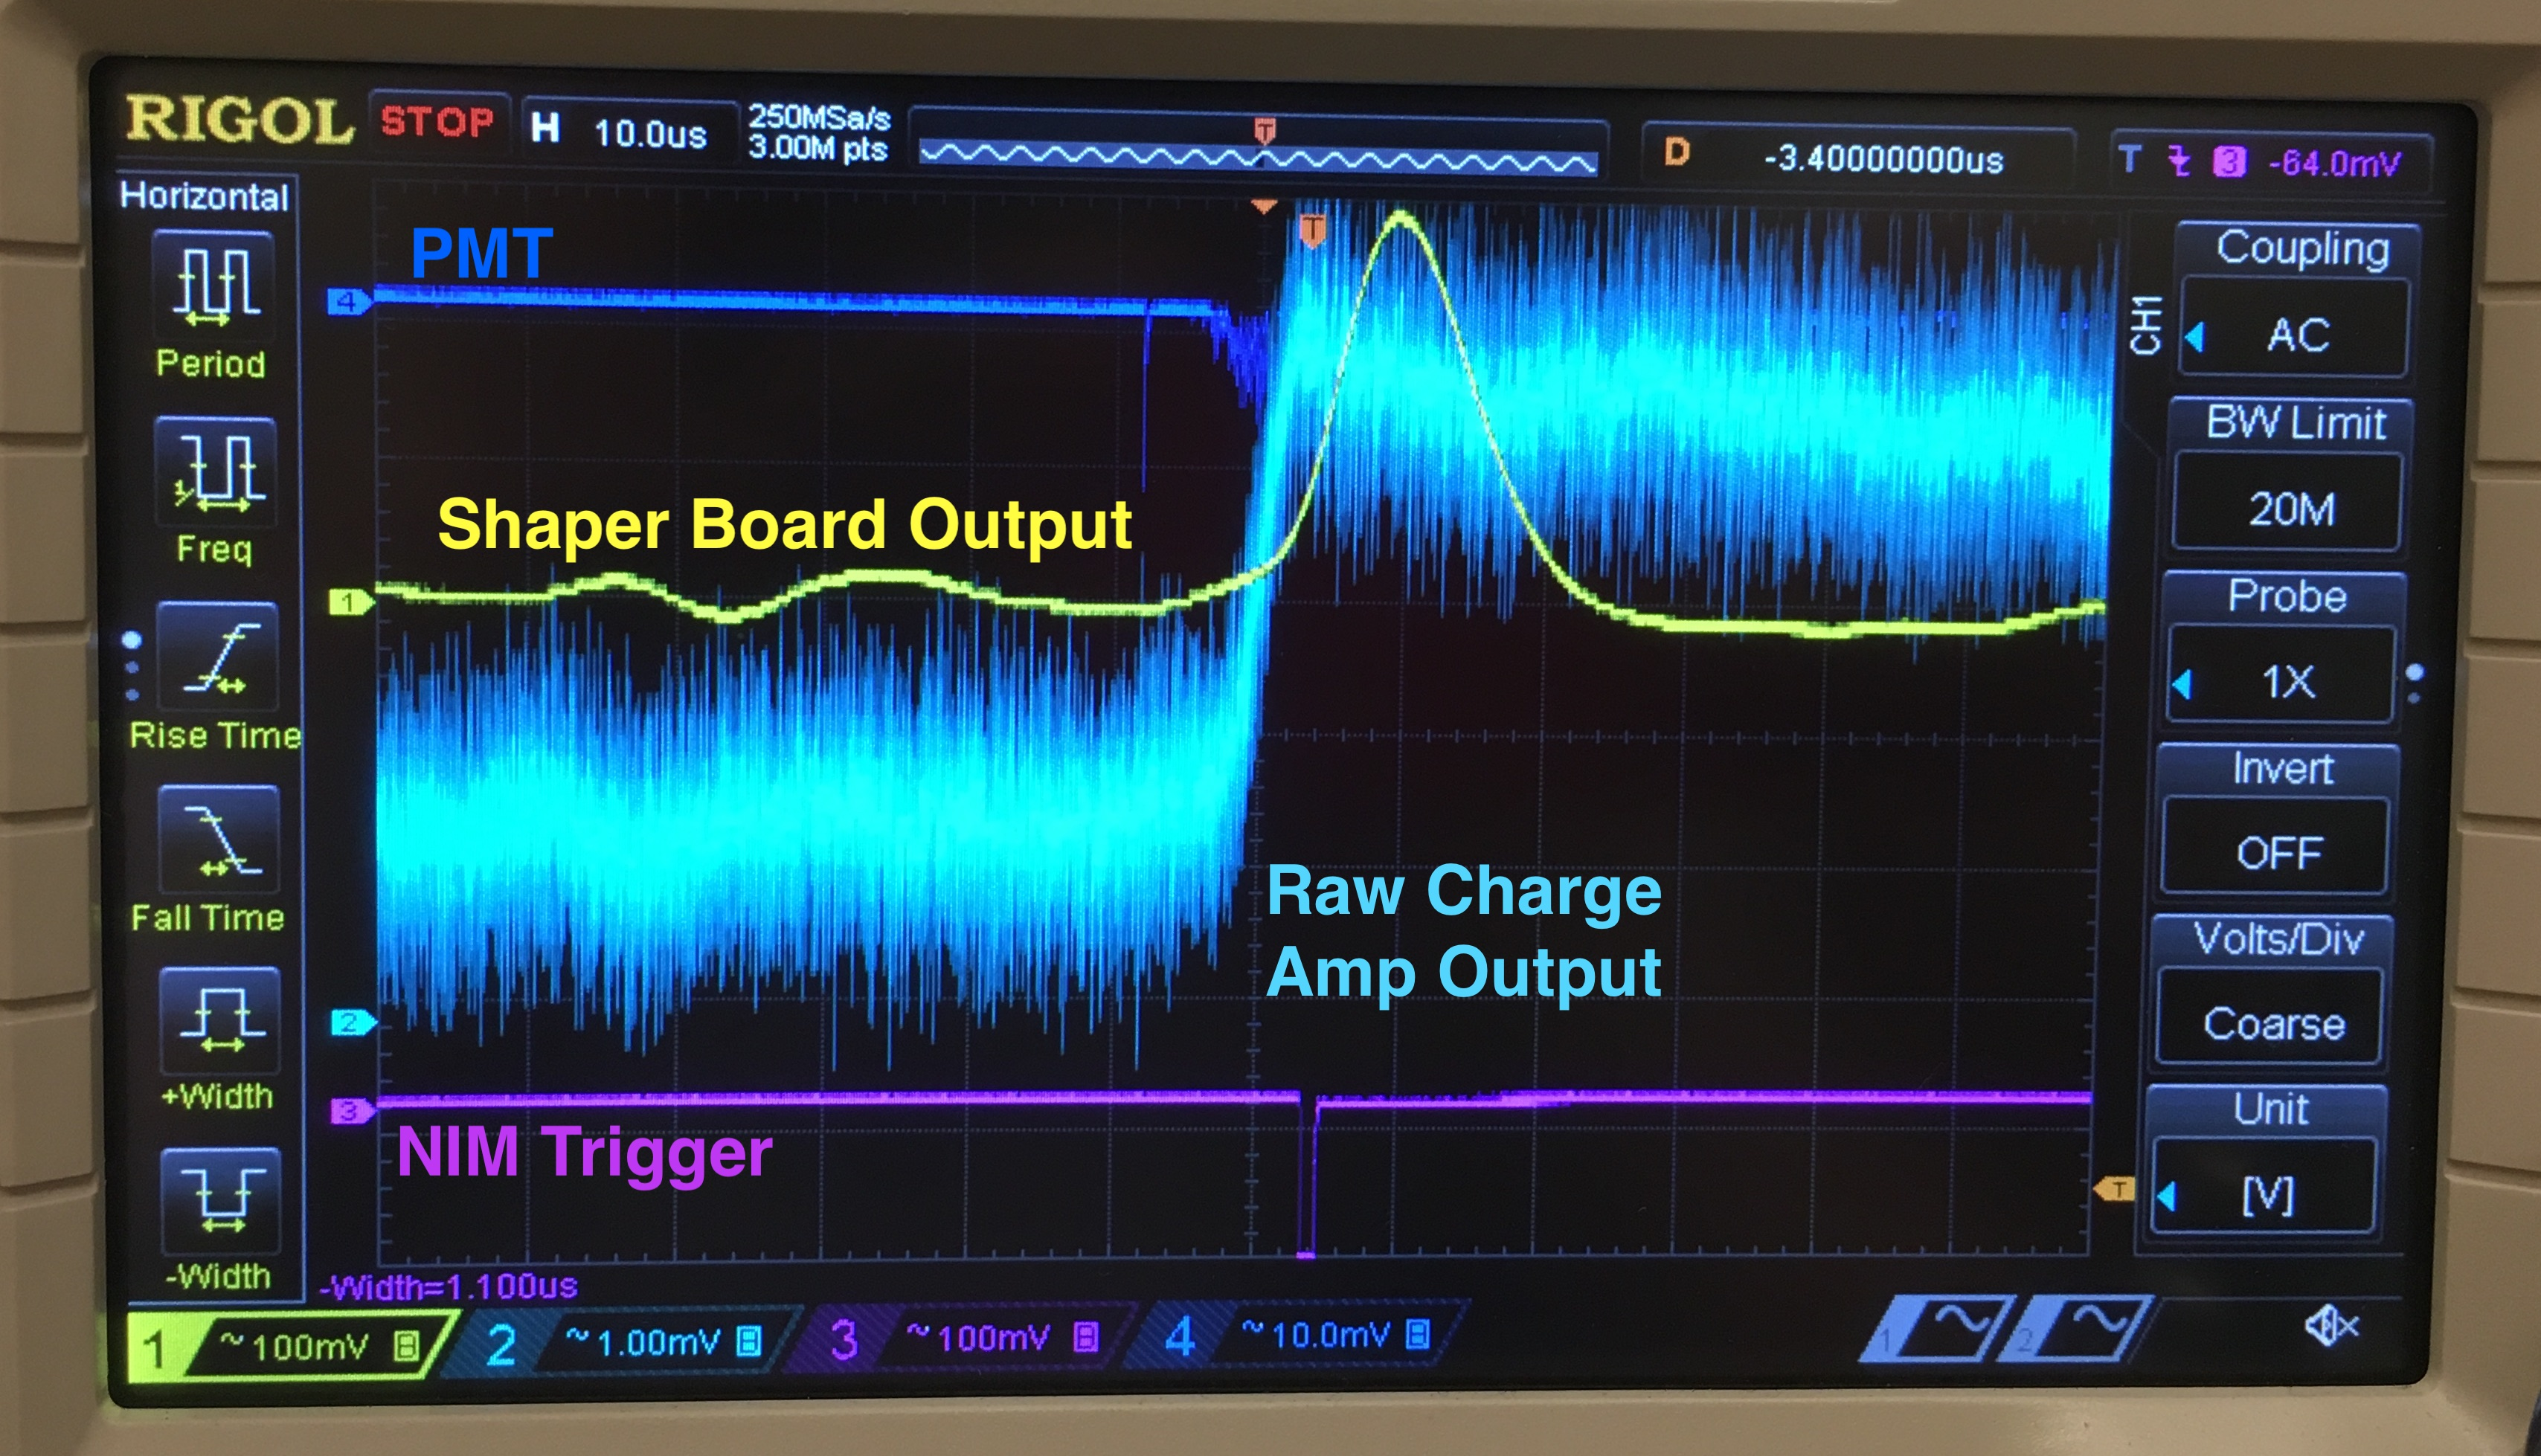
\includegraphics[width=4in]{figures/testbed/charge_amp_shaper.jpg}
\caption{A raw (cyan) and shaped (yellow) charge amp signal taken in -100C gaseous xenon, with the radon source plumbed in. The \acs{PMT} signal is visible in blue and the \acs{NIM} trigger signal is in magenta.}
\label{fig:shaper}
\end{center}
\end{figure}

The charge amplifiers were originally placed inside the experimental vessel, mounted directly on the segmented anode. The functionality of the CR-110 units in \ac{LXe} conditions did not deviate from manufacturer's specifications\footnote{A test was done in a cryogenic fridge to ensure the behavior of the charge amps did not deviate when they were kept at -100~C. There was no change in pulse height (for a fixed input charge), or rise and decay times of the raw signals. This test was not possible in-situ, and so excludes the noise behavior described below, because the manufacturer's test board (CR-150-R5 evaluation board) was necessary to inject charge (via a square wave to an on-board 1~pF capacitor) into the amplifiers.}, however it was found that the units generated enough heat to create a perpetual gas layer under the anode. In general this is not an issue, but for the purpose of the intended absolute electron extraction efficiency measurement, overfilling the \ac{TPC} and using the charge amplifiers as a direct read-out of electrons in the liquid was required. The charge amplifiers were moved to the outer vessel space, surrounded by a small Faraday cage made of copper mesh. See Figure~\ref{fig:chargeamp_mount} for the charge amplifier mounting configurations.

 \begin{figure}[htbp]
\begin{center}
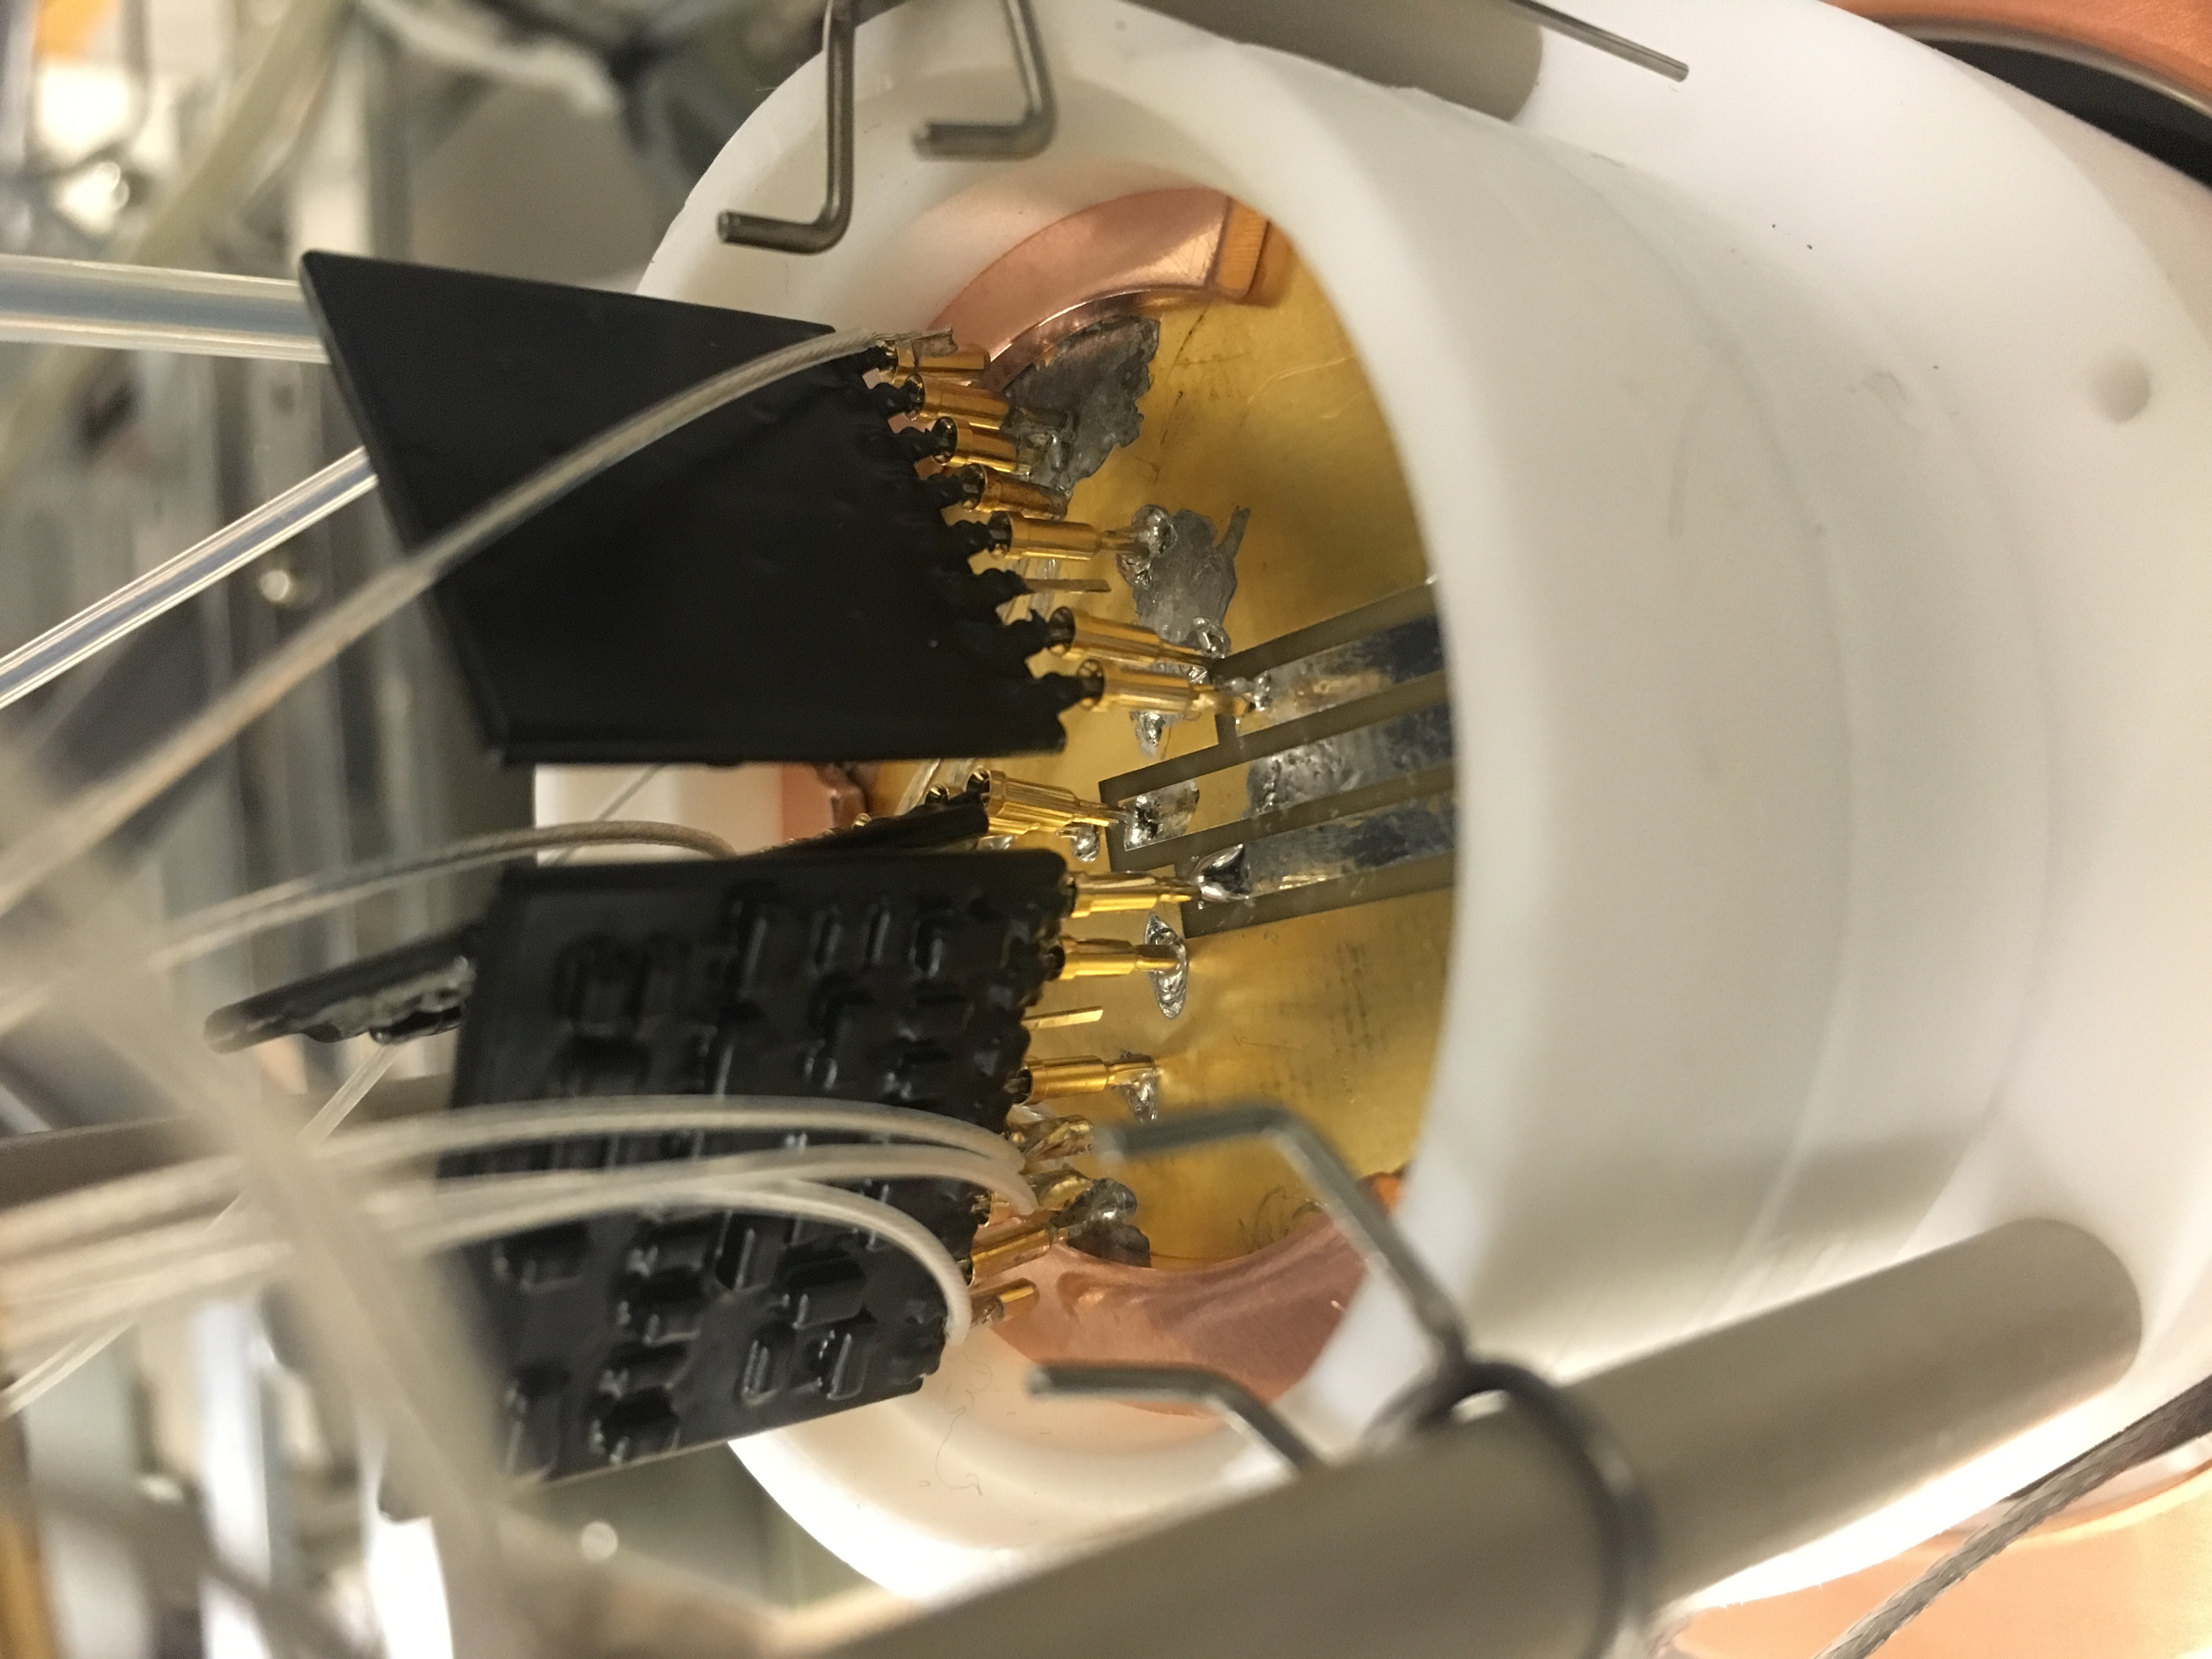
\includegraphics[height=2.5in, keepaspectratio]{figures/testbed/chargeamp_mount1.jpg}
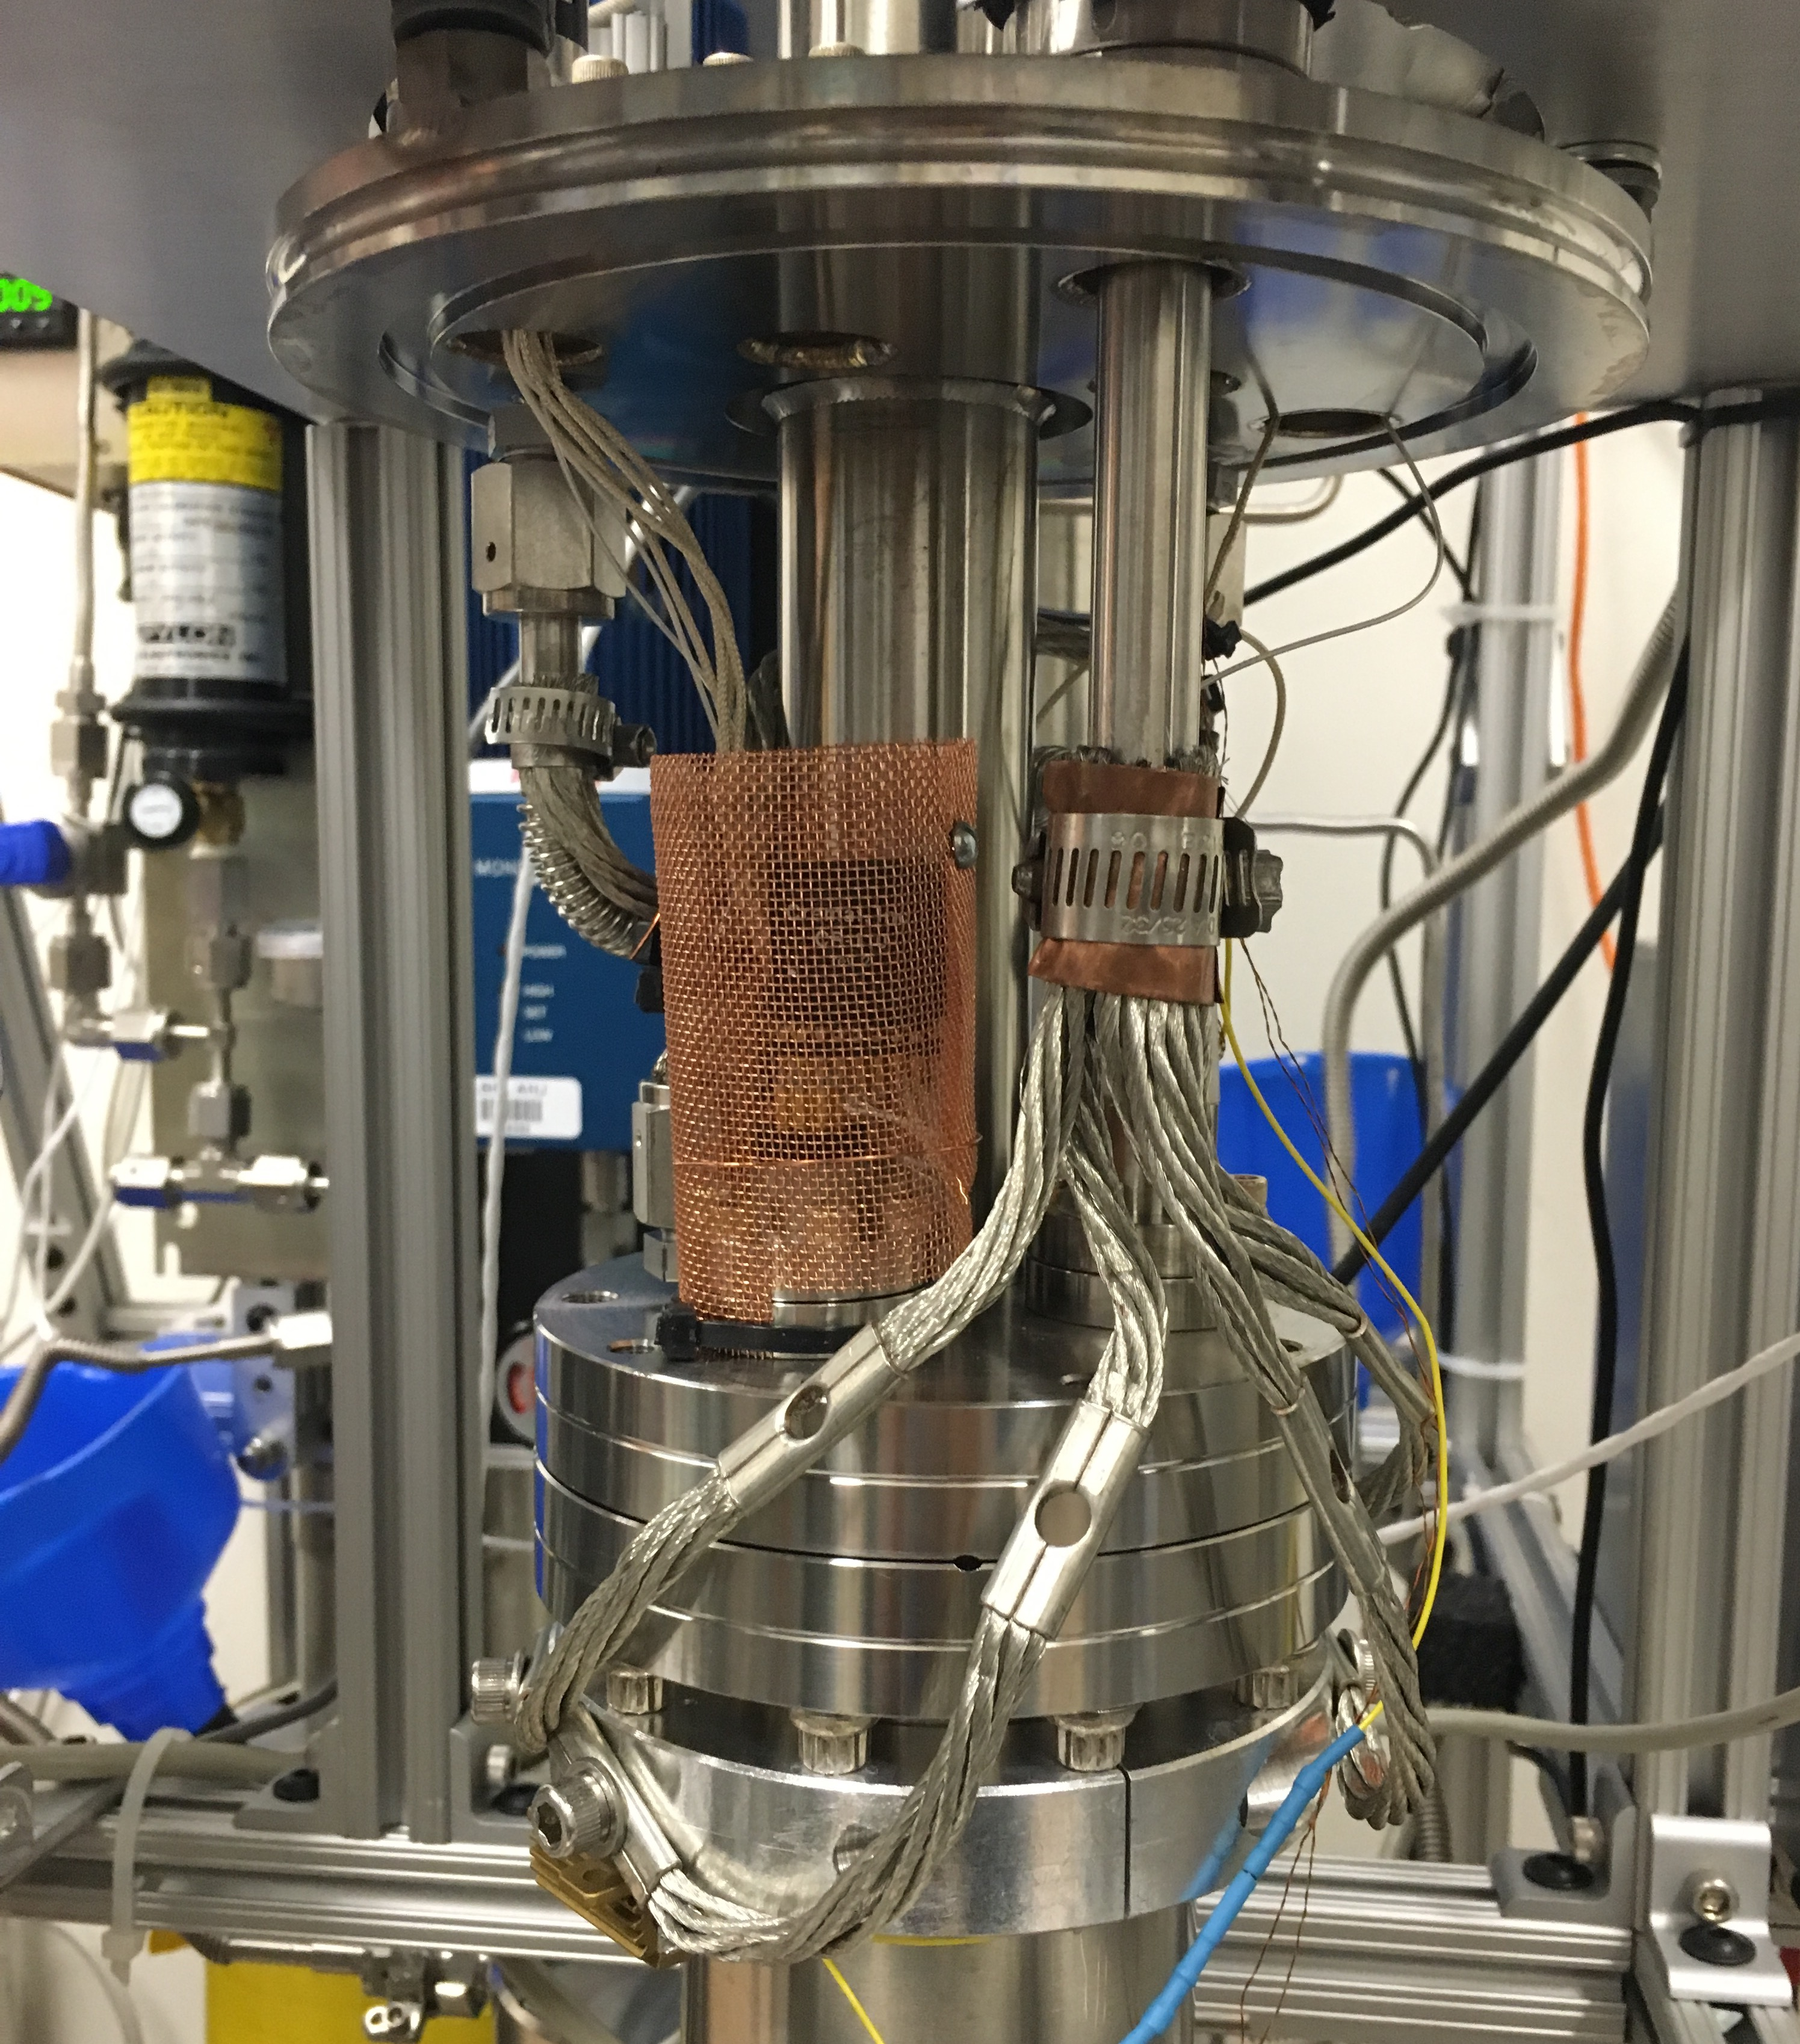
\includegraphics[height=2.5in, keepaspectratio]{figures/testbed/chargeamp_mount2.jpg}
\caption{(left) original mounting of CR-110 charge amplifiers inside the experimental vessel. (right) Mounting in the outer vacuum reduced heat load on the \acs{TPC}. In the outer vessel, the charge amplifiers were surrounded by a Faraday cage constructed from copper mesh to reduce noise.}
\label{fig:chargeamp_mount}
\end{center}
\end{figure}

\subsection{Charge Amplifier Noise Behavior}
Charge amplifiers have baseline RMS noise proportional to the attached capacitance. Figure~\ref{fig:rms} shows the RMS noise of a CR-110 unit attached to different lengths of BNC cable. The longer the cable, the higher the RMS noise. \ac{TPC}s are essentially capacitors, and when filled with \ac{LXe} have a higher capacitance than when the detector is at vacuum. The capacitance of large \ac{LXe} \ac{TPC}s like \ac{LUX} prohibit the use of charge amplifiers for direct readout of the S2 electrons because the RMS noise would swamp the signal. 

\begin{figure}[htbp]
\begin{center}
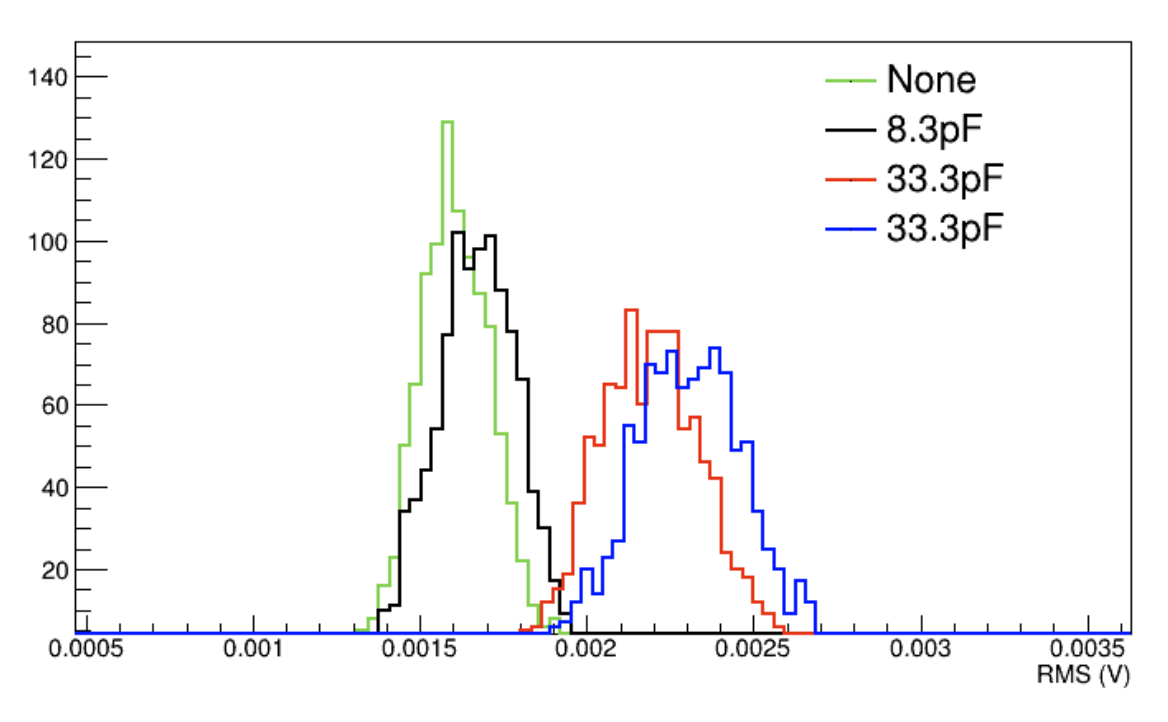
\includegraphics[width=3in]{figures/testbed/rms.png}
\caption{Different lengths of BNC cable attached to a CR-110 test board to show the RMS noise relationship to input capacitance. Two equal length segments (calculated to be 33.3~pF) were observed to have slightly different properties.}
\label{fig:rms}
\end{center}
\end{figure}

Charge amplifiers also respond to acoustics; that is, they are susceptible to microphonic noise. Tapping a finger near a charge amplifier will show as a baseline-jumping response on an oscilloscope. This additional source of noise makes \ac{LXe} \ac{TPC}s challenging places to use charge amplifiers for signal readout because any bubbles in the \ac{LXe} create microphonic signals which the charge amplifiers pick up. By design, dual phase \ac{LXe} \ac{TPC}s are operated near the xenon liquid-gas boundary so the formation and dissipation of gas bubbles in the liquid is likely. Additional sources of acoustic noise like circulation of xenon into the experimental vessel also produce visible responses in charge amplifiers. The difference in micro-acoustic noise environments (gas phase but with/without the circulation pump) is illustrated in Figure~\ref{fig:amp_noise}. The baseline restorer can be seen functioning on the gaussian shaped and amplified signals, but the raw charge signals are subject to baseline wandering (Figure~\ref{fig:amp_noise2}). Figure~\ref{fig:amp_noise2} was taken in a liquid environment during filling, so the effect of bubbles, pressure changes, and other vibrations are visible. 

 \begin{figure}[htbp]
\begin{center}
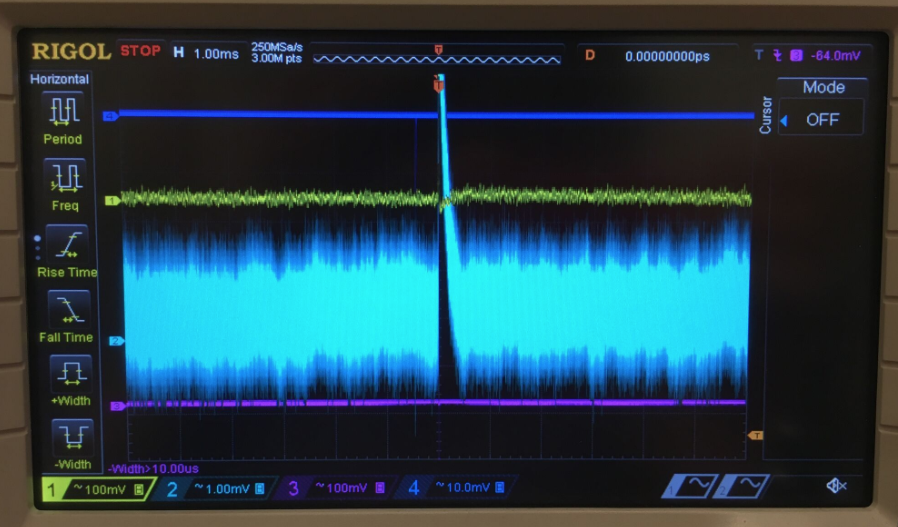
\includegraphics[width = 0.32\textwidth, keepaspectratio]{figures/testbed/circ_off.png}
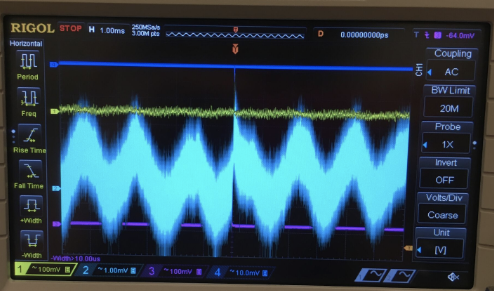
\includegraphics[width = 0.32\textwidth, keepaspectratio]{figures/testbed/circ_noise.png}
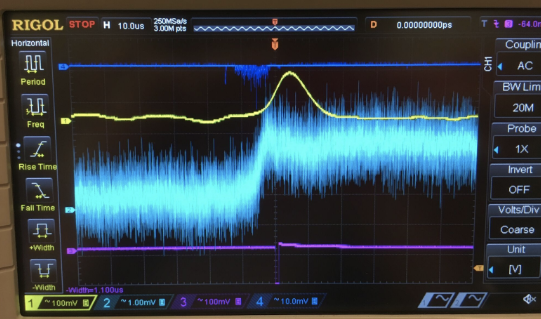
\includegraphics[width = 0.32\textwidth, keepaspectratio]{figures/testbed/circ_noise_zoom.png}
\caption{left) Event showing charge amp with detector -100~C, 1.5~bar, gas only (time scale 1.00~ms/div). (middle) Effect of circulation pump on charge amp is to cause 500~Hz oscillation noise (-100~C, 1.5~bar, gas only (time scale 1.00~ms/div)). (right) Same event as (middle), but zoomed-in time scale (10.0~$\mu$s/div). In all figures, cyan is the raw charge signal (1~mV/div), yellow is the shaped charge (100~mV/div), blue is the \acs{PMT} (10~mV/div) and magenta is the \acs{NIM} trigger (100~mV/div).}
\label{fig:amp_noise}
\end{center}
\end{figure}

 \begin{figure}[htbp]
\begin{center}
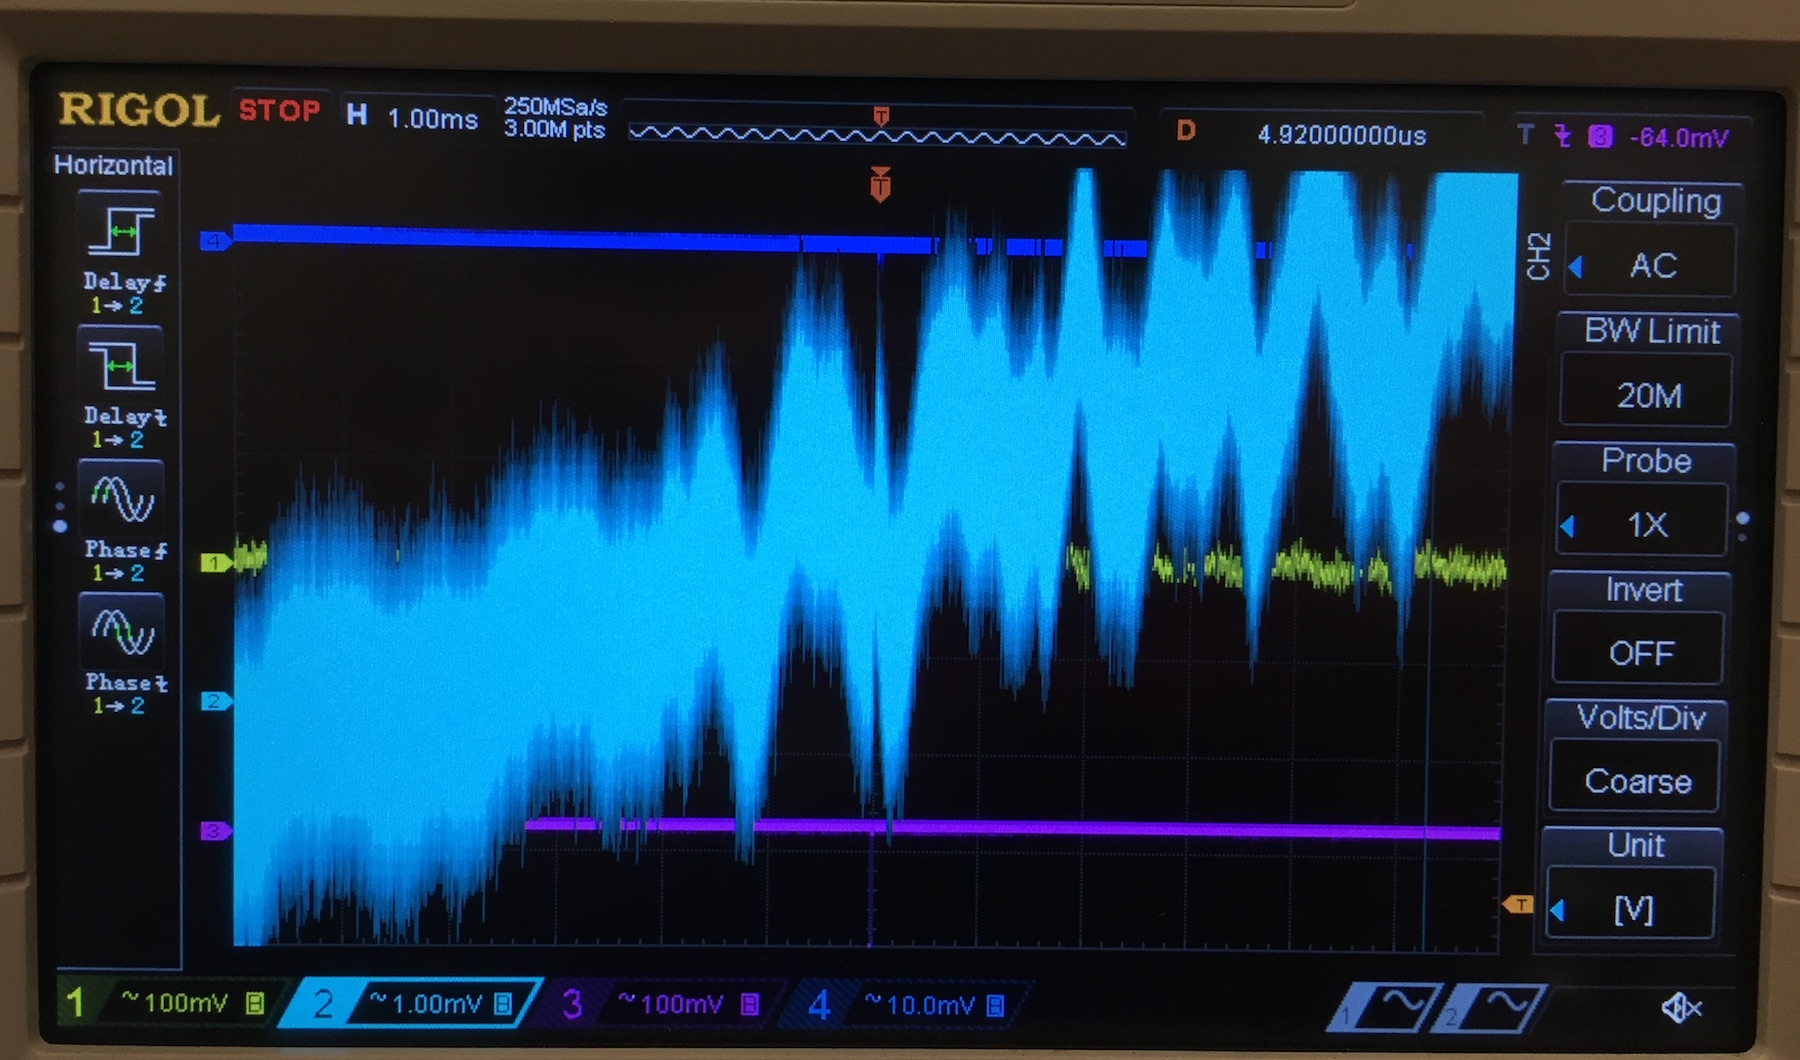
\includegraphics[width = \halffig, keepaspectratio]{figures/testbed/baseline_wander.jpg}
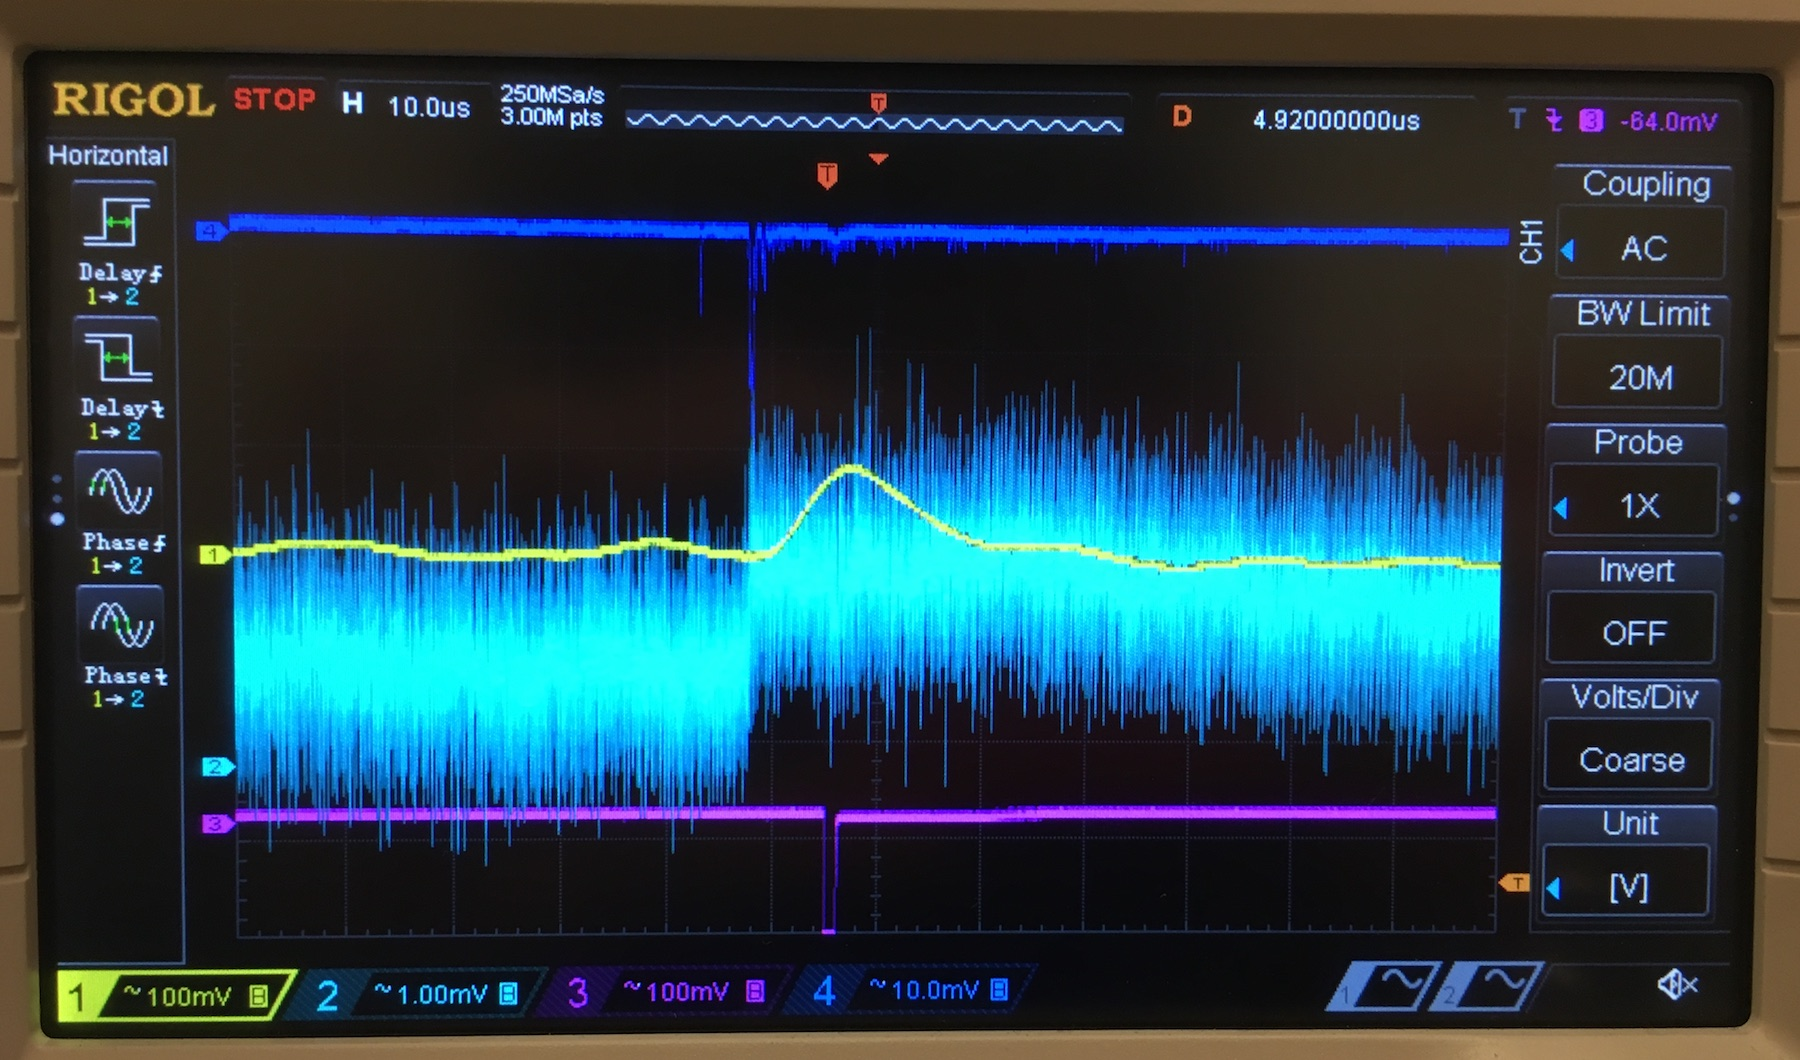
\includegraphics[width = \halffig, keepaspectratio]{figures/testbed/baseline_wander_zoom.jpg}
\caption{An event with the detector at  -100~C, 1.5~bar, with liquid condensed to a level between extraction grid and anode. In both figures, cyan is the raw charge signal (1~mV/div), yellow is the shaped charge (100~mV/div), blue is the \acs{PMT} (10~mV/div) and magenta is the \acs{NIM} trigger (100~mV/div). (left) Scope trace showing a long time view the raw and shaped charge amplifier signals (time scale 1.0~ms/div). (right) Scope trace showing the same event, but zoomed in (10.0~$\mu$s/div). The baseline restorer on the shaped charge signal allowed it to be used as a trigger.}
\label{fig:amp_noise2}
\end{center}
\end{figure}


As \ac{TPC}s are effectively large parallel plate capacitors, any transients coupling to the ``\ac{TPC} capacitor" may be picked up by the charge amplifiers. In particular, instabilities in the \ac{HV} chain induce a current in the \ac{TPC} capacitor that is picked up by the charge amps. Instabilities in \ac{HV} can come from many places. It was observed that for the characteristic capacitance and impedance of the the test bed, partial breakdowns in a length of coaxial \ac{HV} cabling caused a disruption in the functionality of the charge amplifiers. It was also found that a standard laboratory \ac{HV} supply, a Glassman 20~kV negative polarity unit, created pick-up in the charge amplifiers (see Figure~\ref{fig:pickup_noise}).  

 \begin{figure}[htbp]
\begin{center}
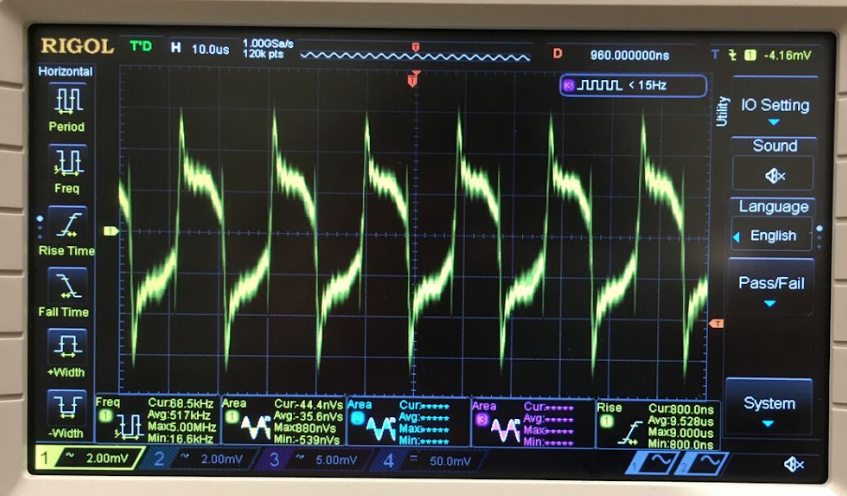
\includegraphics[width = 0.49\textwidth, keepaspectratio]{figures/testbed/glassman_noise.png}
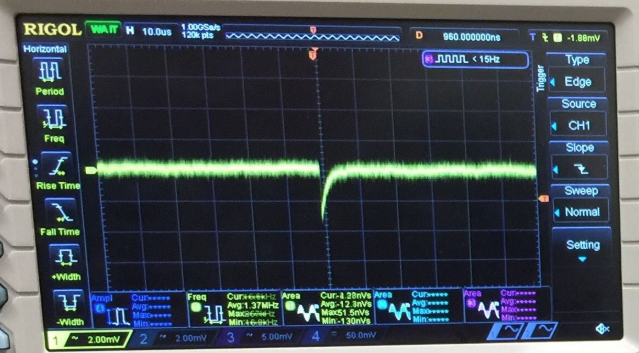
\includegraphics[width = 0.49\textwidth, keepaspectratio]{figures/testbed/partial_breakdown_pickup.png}
\caption{(left) 50~kHz periodic noise from the Glassman 20~kV negative polarity voltage supply. (right) Partial breakdown in coaxial \ac{HV} cable as picked up by charge amplifiers. In both figures, the time scale is 10.0~$\mu$s/div and the voltage scale is 2.00~mV/div.}
\label{fig:pickup_noise}
\end{center}
\end{figure}



%\subsection{\ac{PMT} Saturation}



\section{Data Acquisition and Processing}
Data were acquired with a Picoscope 5000a, a USB-compatible ``oscilloscope." The open source pico-python Python library was used to write voltage records of \ac{PMT} and charge signals to ROOT files, which were opened later for reprocessing into reduced quantities such as pulse area or pulse height. The Picoscope was run as a 14~bit ADC with 125~MHz (8~ns) sampling. For special cases, when only one channel was desired, it was possible to increase the sampling rate to 500~MHZ (2~ns). The manufacturer guide states that the Picoscope can operate in block mode, which uses on-board memory to store events and transfers them to disk only when the on-board memory buffer is full. Block mode is generally preferable to writing each event to disk as it is acquired because the overhead time for USB communication between the Picoscope and write time is only executed once, and so the dead time per event is smaller. However, the block mode capabilities were found to not function and so single event acquisition was used.

\subsection{Estimating Picoscope Dead Time}
Each event was written to disk as it was acquired, which led to a large dead time percentage. The manufacturer provided no information about dead time, but in general, dead times can be estimated in lab using the following method. Trigger the DAQ externally with, e.g., a square wave. Vary the rate of the external trigger, counting how many events are actually recorded by the DAQ in 1 minute. The number of events actually recorded gives the record rate. The record rate will level off at high external trigger rates because it is limited by transfer speed, write time, etc. Subtracting the actual event length from the real total time it takes to record an event gives the dead time per event. When estimating dead times, use the same conditions in data taking, e.g. if 4 channels are used for real data taking, use 4 channels when measuring the record rate. The dead time per acquisition is then the number of events in the acquisition multiplied by the dead time per event. This method is illustrated in Figure~\ref{fig:deadtime}. Such a dead time estimate is used in Chapter~\ref{ch:radon} to calculate the rate in Bq of radon daughters observed.

 \begin{figure}[htbp]
\begin{center}
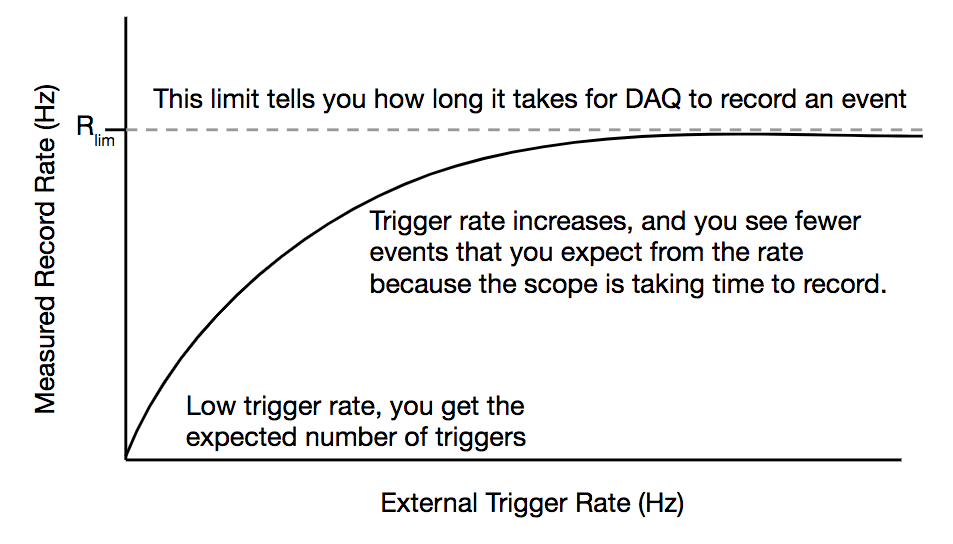
\includegraphics[width =\textwidth ]{figures/testbed/deadtime_plot.png}
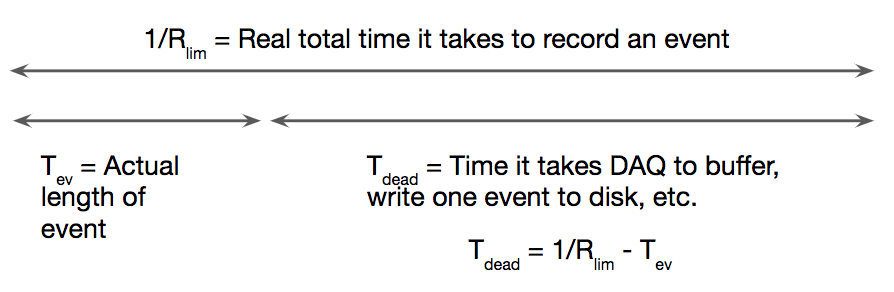
\includegraphics[width =\textwidth]{figures/testbed/deadtime_math.png}
\caption{(top) Laboratory method to find the maximum \acs{DAQ} record time time. (bottom) Calculating dead time from maximum record rate.}
\label{fig:deadtime}
\end{center}
\end{figure}


\subsection{PMT Signal Processing}
A simple pulse finder was written in Python. Instead of searching for pulses left-to-right along a signal trace, the algorithm found the maximum of the trace, and then searched left and right until the trace went below a threshold. After these edges were identified, the trace was set to zero for the duration of the pulse, and then the next-tallest pulse was sought. Pulses were found until there were no more, or the number found was equal to some user-defined number of pulses. Thus, pulse starts and stops were acquired for each \ac{PMT} trace. These pulse starts and stops were then used to calculate useful \ac{RQ}s such as pulse area, width, prompt fraction, etc. S1 and S2 identification was done later, based on these \ac{RQ}s. The definitions of S1, S2, and other high-level \ac{PMT} \ac{RQ}s were specific to the state of the test bed hardware, which was typically changed on a weekly basis during development. A stable data processing framework was not maintained. 

\subsection{Charge Amplifier Signal Processing}
\label{sec:charge_amp_processing}
The shaped charge amplifier signals were used primarily as a trigger throughout the studies in Chapter~\ref{ch:radon} and Chapter~\ref{ch:etrains}. They were originally acquired and implemented because the raw charge signals were small and difficult to process. This was due to field strength, purity, and grid transparency; these issues are described in more detail in Chapter~\ref{ch:etrains}, but were all essentially solved by removing the grid to produce an ``extraction region only'' configuration (Figure~\ref{fig:internals} (right)). Various methods were explored to process the raw signals into the relevant charge \ac{RQ}: step height (mV), which could then be translated to charge (Coulombs, then number of electrons) per the manufacturer's specifications. For small, raw charge signals a fit function was found to out-perform a simple step algorithm; for larger raw signals the step algorithm was fast and robust. Both methods are illustrated below, the fit function in Figure~\ref{fig:charge_fit} and the step algorithm in Figure~\ref{fig:charge_algorithm}. 

The fit function was a piece-wise defined linear function plus a falling exponential. The linear function was defined to be zero before some offset time $t_{o}$, and after the offset time plus rise time of the charge trace ($t_{o} + t_{r}$). The exponential was zero before $t_{o} + t_{r}$, and the two functions had equal values at $t_{o} + t_{r}$. 

The step algorithm produces a new trace with peak instead of a step by averaging a user-defined number of samples, $n_{s}$, of the original charge amp voltage trace from $[i+n_{s},i+2n_{s}]$ and subtracting the average of the waveform from a previous section, $[i,i+n_{s}]$. If $n_{s}$ is chosen to be exactly the rise time of the trace, then the maximum of the new trace is equal to the step height. See Figure~\ref{fig:nsamp_choice} for examples of two different choices of $n_{s}$. In practice, it is difficult to choose $n_{s}$ perfectly because noise plays a large role; it was easier instead to find the peak of the new trace to locate the approximate step position of the original trace based on $n_{s}$, and take the average of several samples as the step height (Figure~\ref{fig:charge_algorithm}). That is, if $n_{p}$ is the location of the peak after the step-finding algorithm, the approximate location of the step is $n_{p} + 2n_{s}$. 

 \begin{figure}[htbp]
\begin{center}
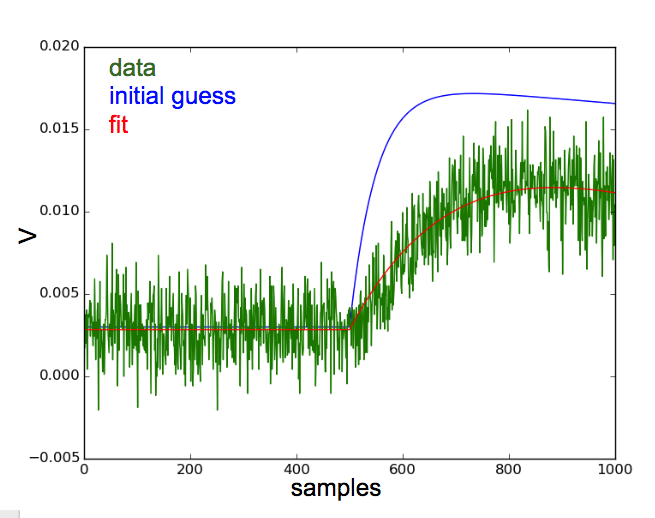
\includegraphics[width =\textwidth ]{figures/testbed/charge_fit.png}
\caption{Fitting the charge traces with a piece-wise defined linear rise and exponential fall. 1 sample is 8~ns.}
\label{fig:charge_fit}
\end{center}
\end{figure}

 \begin{figure}[htbp]
\begin{center}
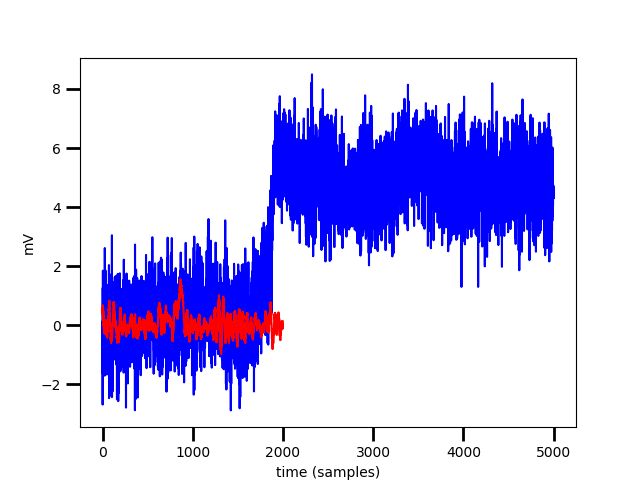
\includegraphics[width =\halffig ]{figures/testbed/figure_q20.png}
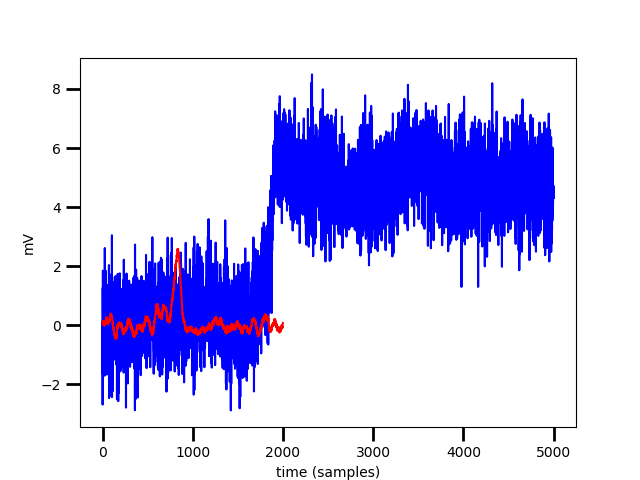
\includegraphics[width =\halffig ]{figures/testbed/figure_q50.png}
\caption{The step-finding algorithm shown with a choice of 20 samples averaged (left) and with 50 samples averaged (right). If $n_{s}$ is chosen to be the rise time of the pulse, the height of the output waveform is the height of the step. These step algorithms actually include an offset, $n_{o}=1000$, so the averages are taken from $[i+n_{o}+n_{s},i+n_{o}+2n_{s}]$ and $[i+n_{o},i+n_{o}+n_{s}]$. Alternatively, a smaller number can be chosen for $n_{s}$, and the location of the maximum of the output waveform can be used to find the location of the top of the step (shown in Figure~\ref{fig:charge_algorithm}). 1 sample is 8~ns. }
\label{fig:nsamp_choice}
\end{center}
\end{figure}

 \begin{figure}[htbp]
\begin{center}
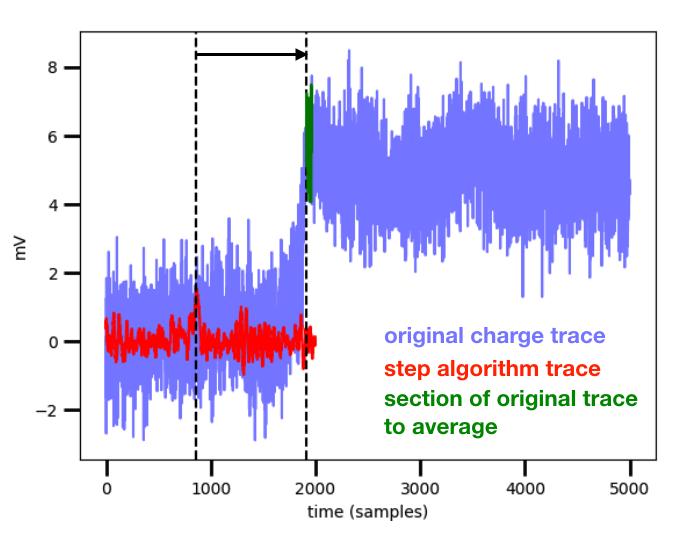
\includegraphics[width =\textwidth ]{figures/testbed/charge_algorithm.png}
\caption{The location of the top of the step can be robustly found from the location of maximum of the step-finding algorithm. Some number of samples at the top of the step can be averaged to give the step height. 1 sample is 8~ns. This particular example uses $n_{s}=20$. The step-finding algorithm is calculated with an offset, $n_{o}=1000$, so the averages are taken from $[i+n_{o}+n_{s},i+n_{o}+2n_{s}]$ and $[i+n_{o},i+n_{o}+n_{s}]$. If the peak location (red peak) is $n_{p}$, then the approximate location of the step is $n_{p} + n_{o} + 2n_{s}$, and some number of samples of the original trace (50 samples shown in green) can be averaged to give the step height. }
\label{fig:charge_algorithm}
\end{center}
\end{figure}


Another source of charge amplifier noise is the Shockley-Ramo effect. The Shockley-Ramo effect refers to the Shockley-Ramo theorem, which says that the instantaneous current $i$ and charge $Q$ induced on a given electrode due to the motion of a charge is \cite{He2001}:

\begin{equation}
\begin{split}
i &= q\vec{v} \cdot \vec{E_{0}}(\vec{x}) \\
Q &= -q V_{0}(\vec{x})
\end{split}
\end{equation}
where $q$ is the charge, $\vec{v}$ is the instantaneous velocity of the charge, and $\vec{E_{0}}(\vec{x})$ and $V_{0}(\vec{x})$ are the electric field and potential that would exist at $q$'s instantaneous position $\vec{x}$ under the following circumstances: the electrode of interest is at 1~V, all others are at 0~V, and all charges are removed. A helpful review of Shockley-Ramo and a discussion about its effect on charge sensing techniques can be found in \cite{He2001}. The charge amplifiers are an integrator circuit, and the Shockley-Ramo theorem implies that even if a charge isn't directly underneath a given anode segment, that anode segment has field lines terminating on it as a result of the motion of the charge, and therefore an induced current. When an electron terminates on an anode segment, the other segments ``see'' the field reduction and register it as a positive charge, or an electron moving in the opposite direction; the response is a dip in the trace. For the gaussian shaping amplifiers, the Shockley-Ramo effect was more evident, and can be corrected for by adjusting the maximum for any following dip; on the raw traces, it is more difficult to account for. The dips are present in the raw traces, but in general much less visible and aren't corrected for. In the amplified and gaussian-shaped traces, the dip is more visible, as in Figure~\ref{fig:shockley_ramo}.  

 \begin{figure}[htbp]
\begin{center}
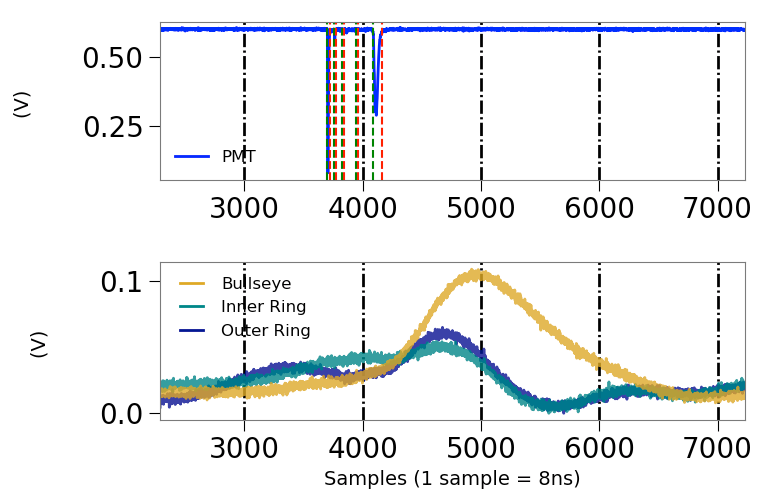
\includegraphics[width =\textwidth ]{figures/testbed/shockley_ramo.png}
\caption{An alpha event showing the Shockley-Ramo effect on the inner and outer ring segments of the anode. The top plot shows the \acs{PMT} trace and the bottom plot shows the shaped response of the anode segments. The Schockley-Ramo effect is the rise (around 4700~samples) and subsequent dip (around 5500~samples) of the inner and outer ring traces. The event happened under the bullseye segment, but the other traces see the field line density increase and then disappear, producing both an increase and decrease in the shaped anode signal.  }
\label{fig:shockley_ramo}
\end{center}
\end{figure}


The gains of the gaussian shaping amplifiers were not extensively characterized because they were never used to reconstruct a physical quantity. The shaping amplifiers were used primarily as a trigger because the unit had a baseline restorer, which the raw charge amplifiers did not (see Figure~\ref{fig:amp_noise} and Figure~\ref{fig:amp_noise2} for the noise conditions on shaped and raw charge amplifiers).

\section{High Voltage Feedthrough Design}
A significant amount of time was spent developing and testing \ac{HV} feedthroughs for the test bed. This section describes a few of the feedthroughs that were unsuccessful, leading to the final design, which is capable of delivering -11~kV to the cathode with no observable breakdown or other effects. Extensive detail of the tests and procedures are not provided. Instead, the following vignettes are intended as an overview to be useful to a student tasked with designing a \ac{HV} feedthrough. 

\subsection{Off The Shelf Feedthroughs}
The first attempts at building feedthroughs were to use off-the-shelf products from typical vacuum supply vendors such as MDC Vacuum and Kurt J. Lesker. Vacuum \ac{HV} feedthroughs are intended for use from air to vacuum, not air to \ac{LXe}; we were attempting to operate them outside of their intended usage parameters. Additionally, by combining ceramic and metal (typically aluminum, stainless steel, nickel, copper) they are especially prone to breakdown at the meeting of these different materials, known colloquially as ``triple points''. When there are interfaces between materials with different permittivities (dielectric constants), the electric fields are distorted. Electric field is ``pushed'' out of the higher dielectric material into the lower dielectric material. This creates a field enhancement where peak fields can be much higher than average fields in the system. The field enhancement from triple points where there is in interface between a conductor and two different dielectrics (e.g conductor, ceramic insulator, and gaseous Xe) is a common source of breakdown along insulator surfaces. Good design practices, namely choices of geometry, reduce the field enhancements in these regions. With commercial feedthroughs, the geometry choice is set and may not be sufficient for the task.

Note that ceramic feedthroughs are not appropriate for low background experiments due to their high radioactivity. For test beds, where low radioactivity is not a priority, ceramic feedthroughs may be used.

The first few feedthroughs used a 12~kV \ac{SHV} weldable feed though as shown in Figure~\ref{fig:12kV-SHV}. If used as operation is intended, the side indicated by A is used on the vacuum-side and B connects to the voltage supply. Instead, we trimmed the long B side and attached a copper, screw-port connector to make the 90 degree connection from vertical feedthrough to horizontal grid. This was done to avoid placing a conducting surface at high voltage (the cap on the ceramic on side A) in gaseous xenon, thereby increasing the risk of breakdown to the walls of the detector. The feedthrough's vertical placement is designed such that the copper connector is fully submersed in \ac{LXe} (Figure~\ref{fig:ft1}).

 
\begin{figure}[htbp]
\begin{center}
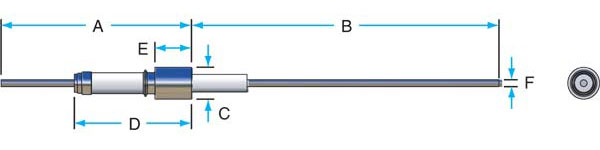
\includegraphics[width=5in]{figures/testbed/12kV-SHV.jpg}
\caption{A 12kV SHV weldable connector from vacuum supplier Kurt Lesker.}
\label{fig:12kV-SHV}
\end{center}
\end{figure}

\begin{figure}[htbp]
\begin{center}
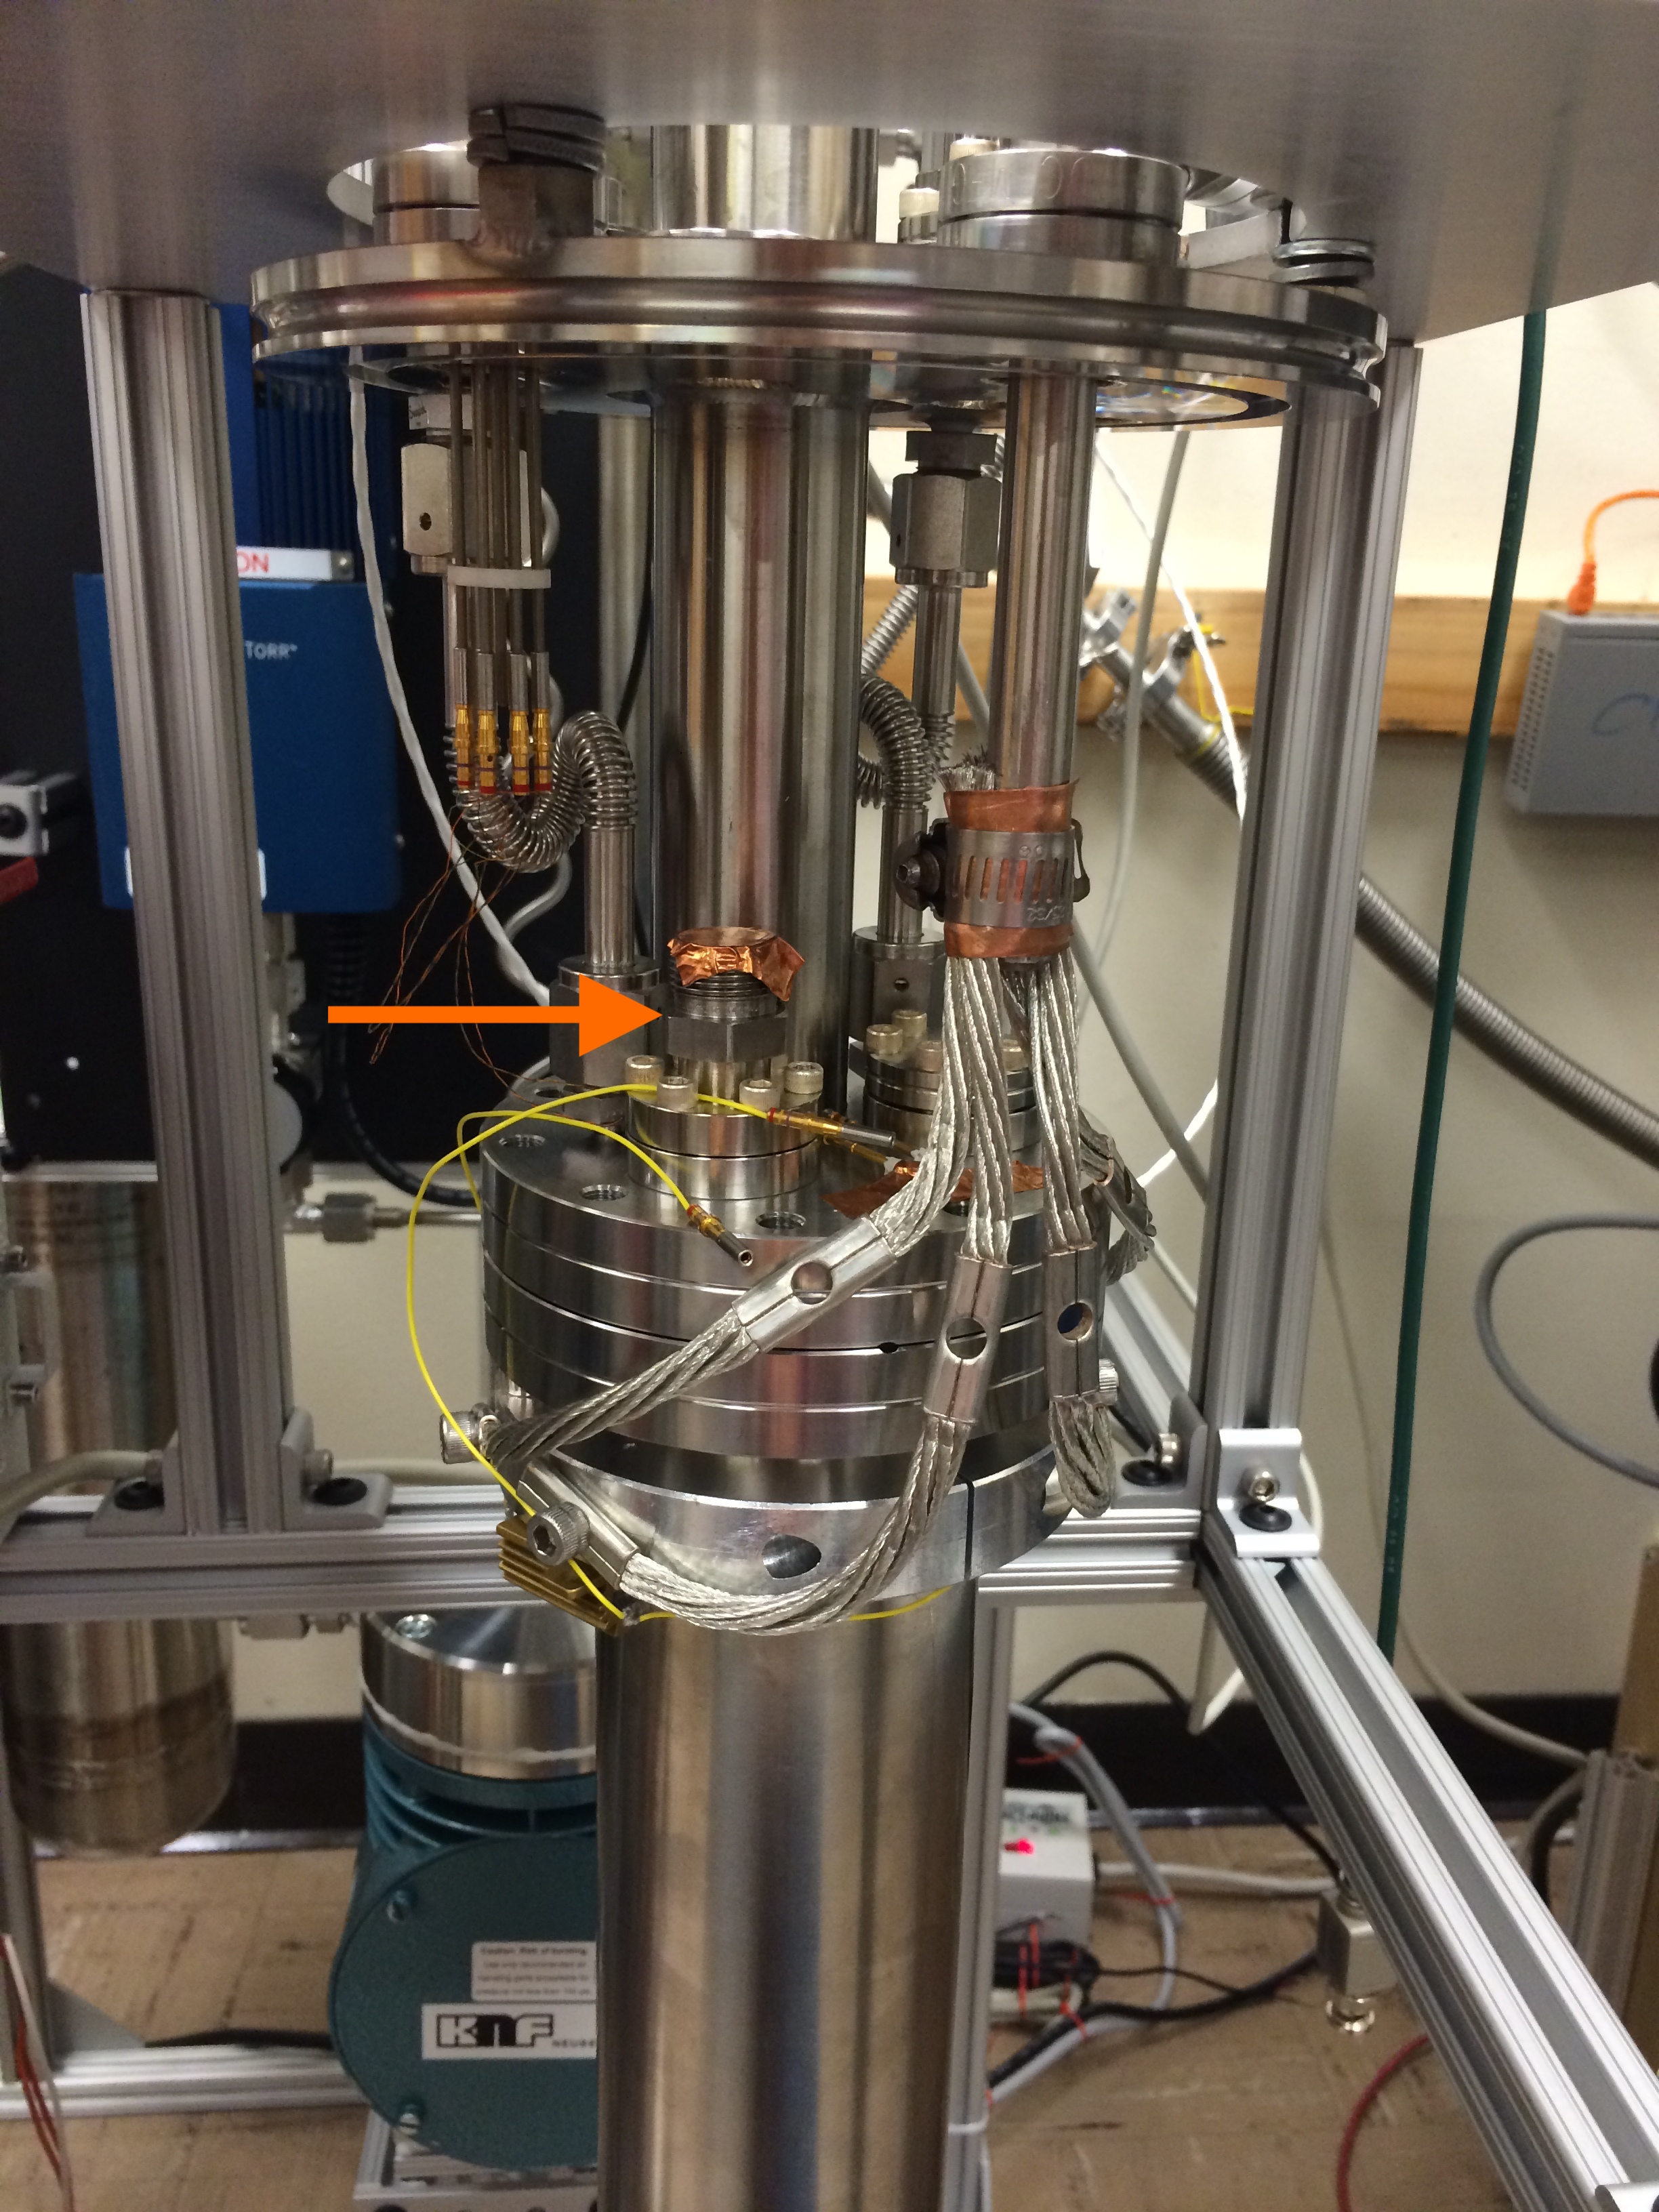
\includegraphics[width=0.49\textwidth]{figures/testbed/ft1_2.jpg}
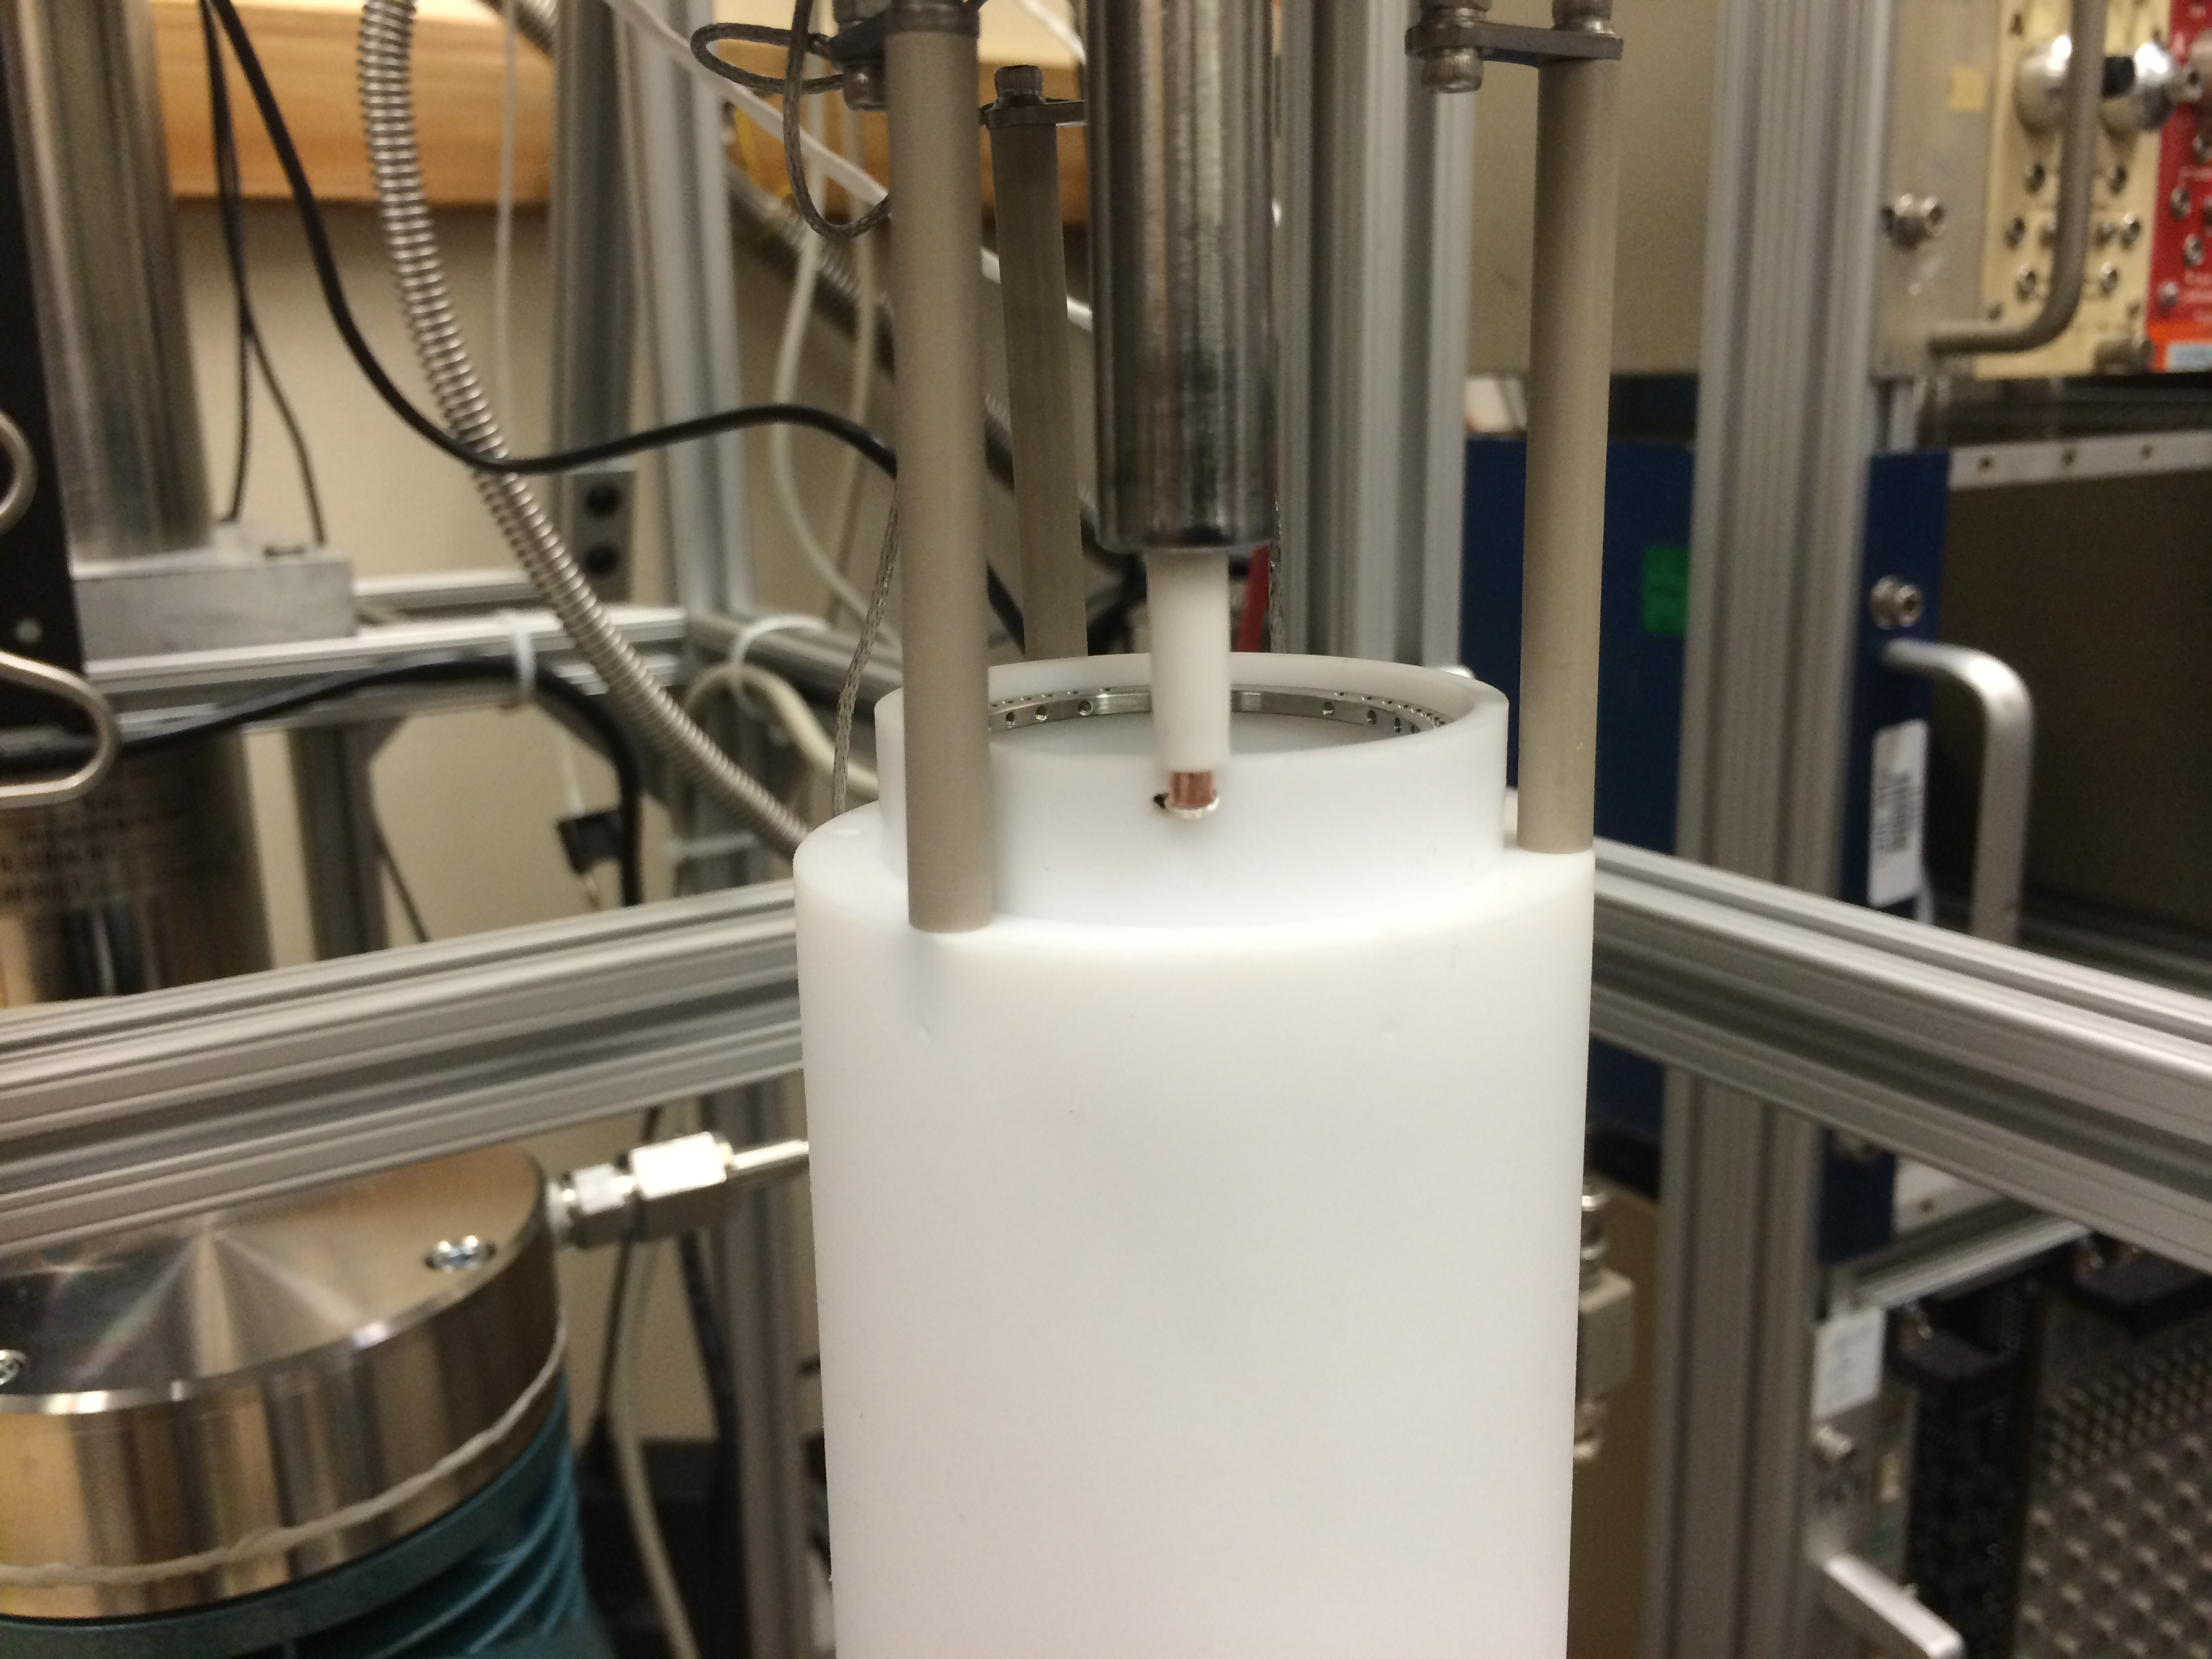
\includegraphics[width=0.49\textwidth]{figures/testbed/ft1_1.jpg}
\caption{(left) The copper tape in this picture is sitting on top of a 1/2~inch swage connector (indicated by the arrow). The swage connector captures a 1/2~in pipe, which has the 12~kV \acs{SHV} feedthrough welded to the end. (right) 12~kV \acs{SHV} weldable connector, inverted, clipped, and attached with a machined copper connector. The connector uses a screw to capture the \acs{SHV} feed though, and the same screw to capture a stranded wire, visible in this picture as the silver strands on the copper tip, which is then fed through a hole drilled in the \acs{PTFE} to connect to the wire grid frames. The wire was wrapped around the grid frame. }
\label{fig:ft1}
\end{center}
\end{figure}

%\begin{figure}[htbp]
%\begin{center}
%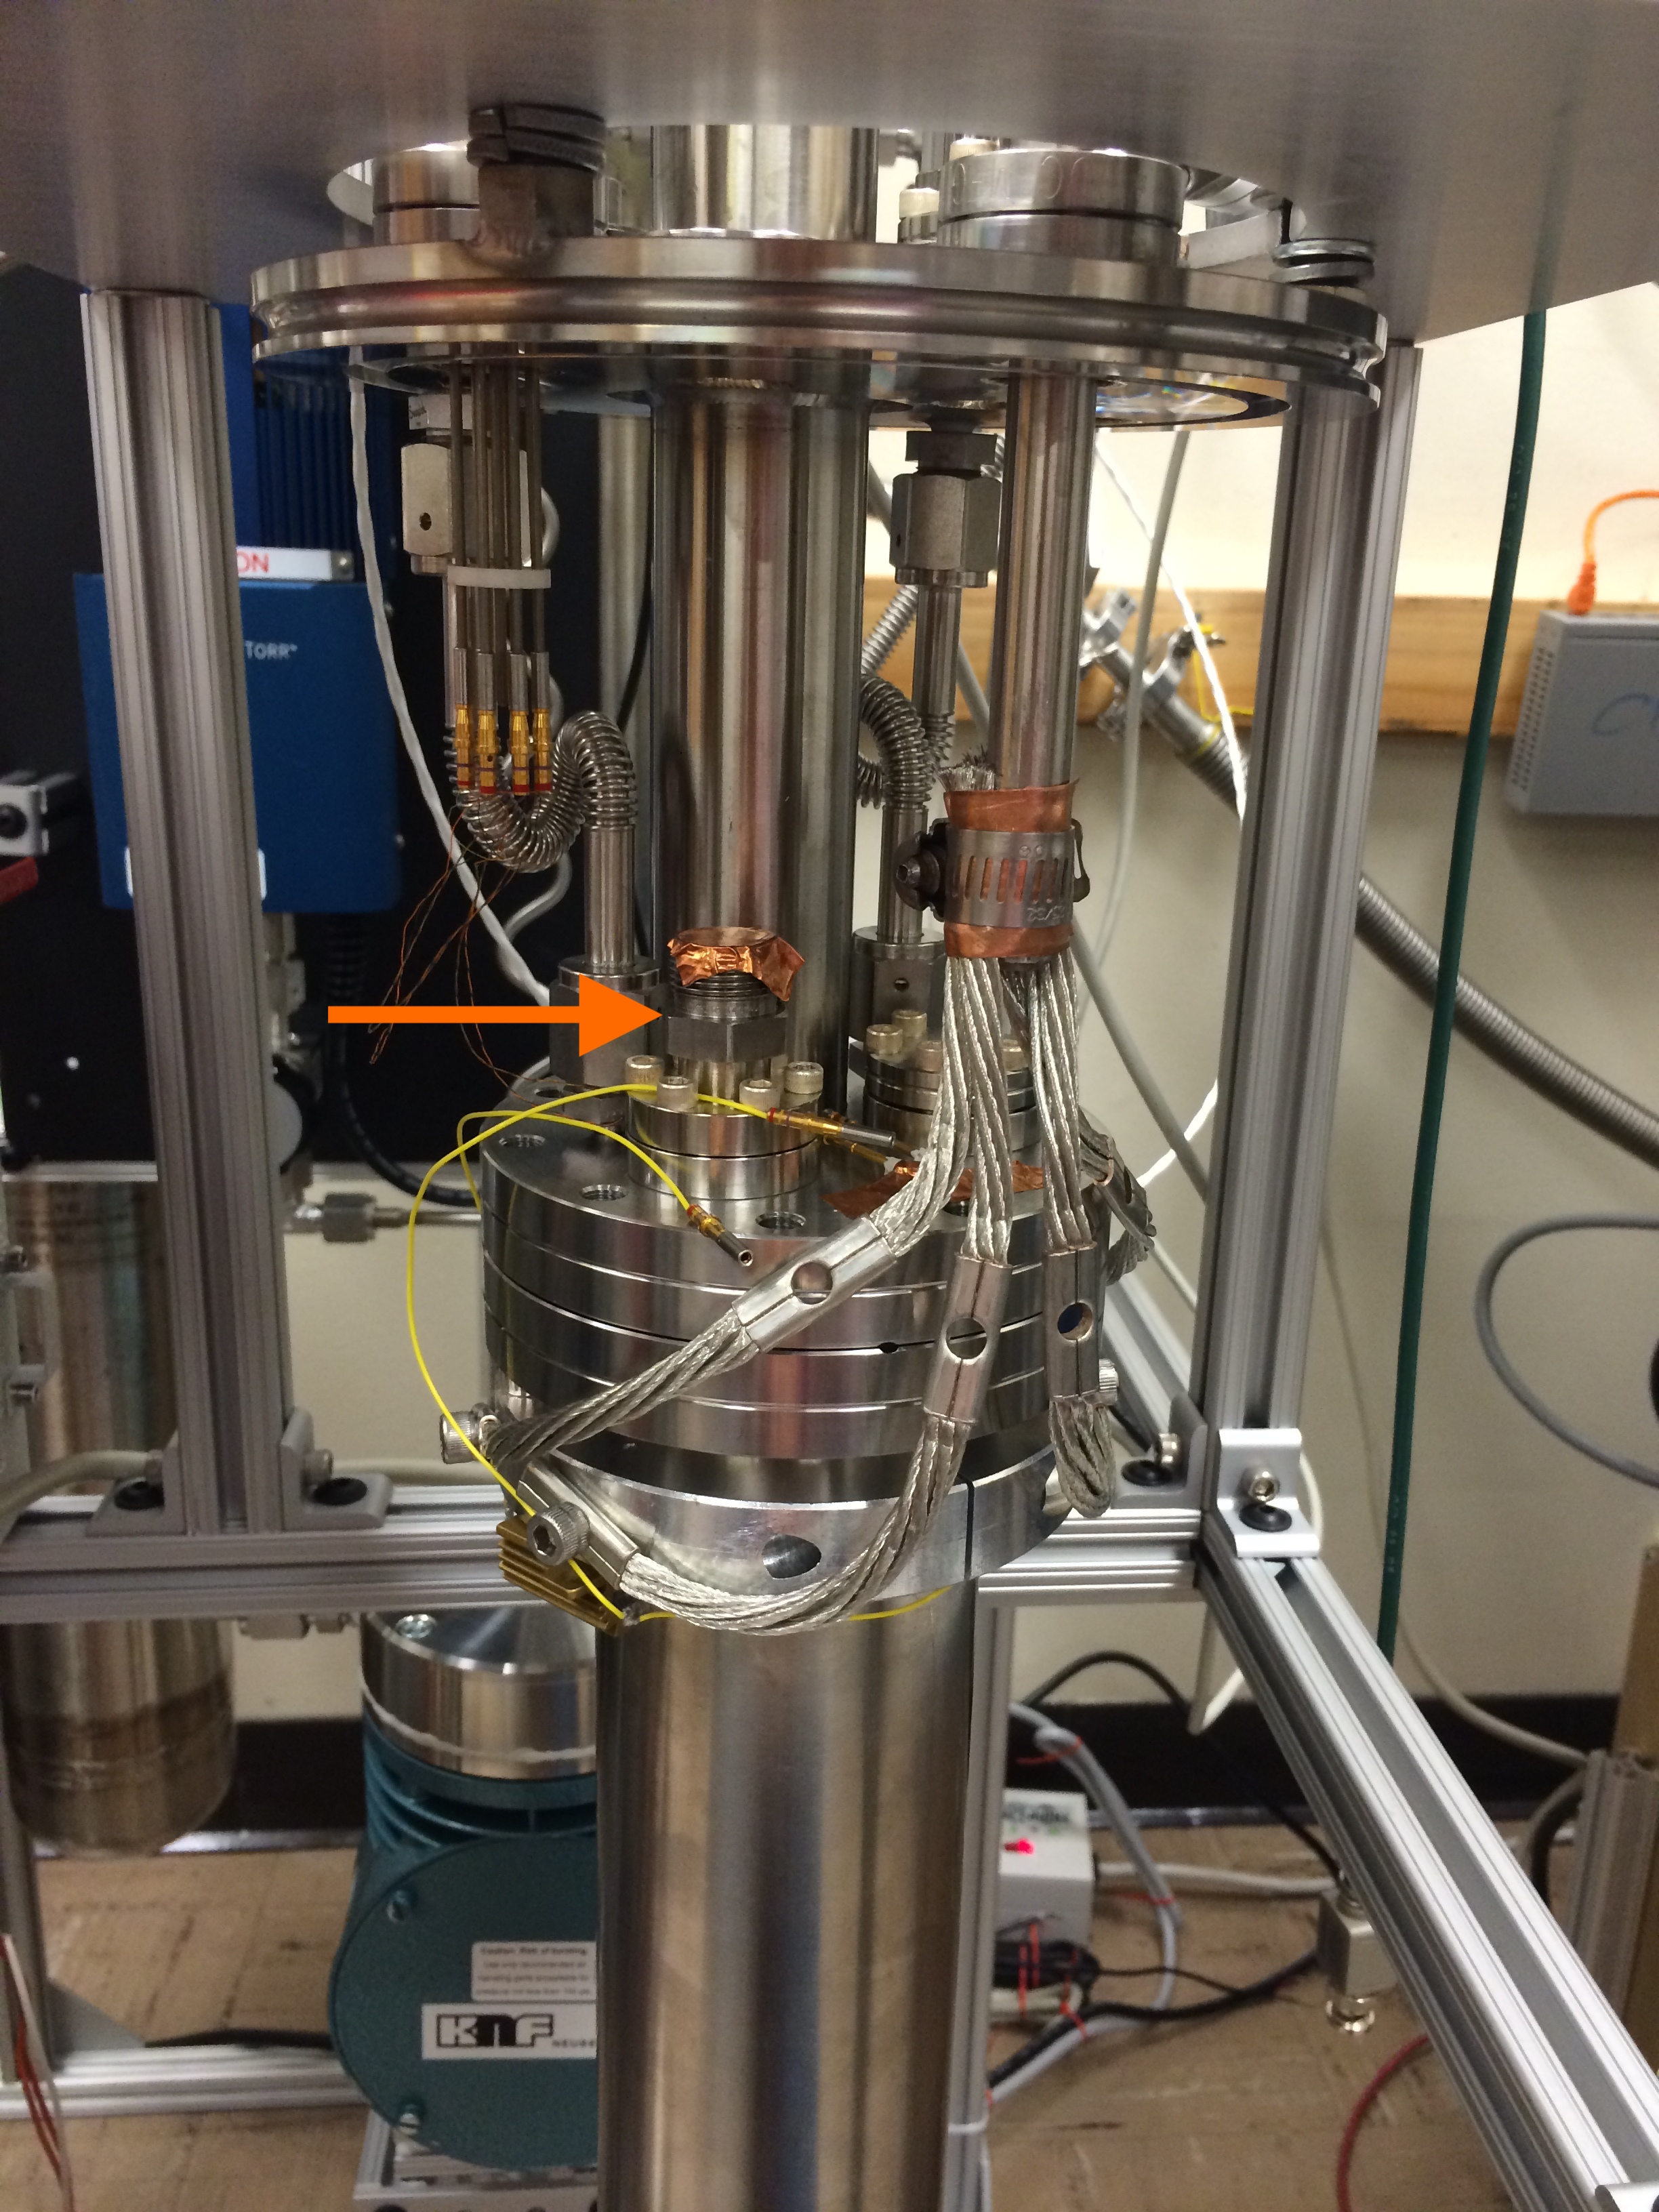
\includegraphics[width=\textwidth]{figures/testbed/ft1_2.jpg}
%\caption{The copper tape in this picture is sitting on top of a 1/2~-in swage connector. The swage connector captures a 1/2~in pipe, which has the 12kV SHV feedthrough welded to the end.}
%\label{fig:ft1_2}
%\end{center}
%\end{figure}

\begin{figure}[htbp]
\begin{center}
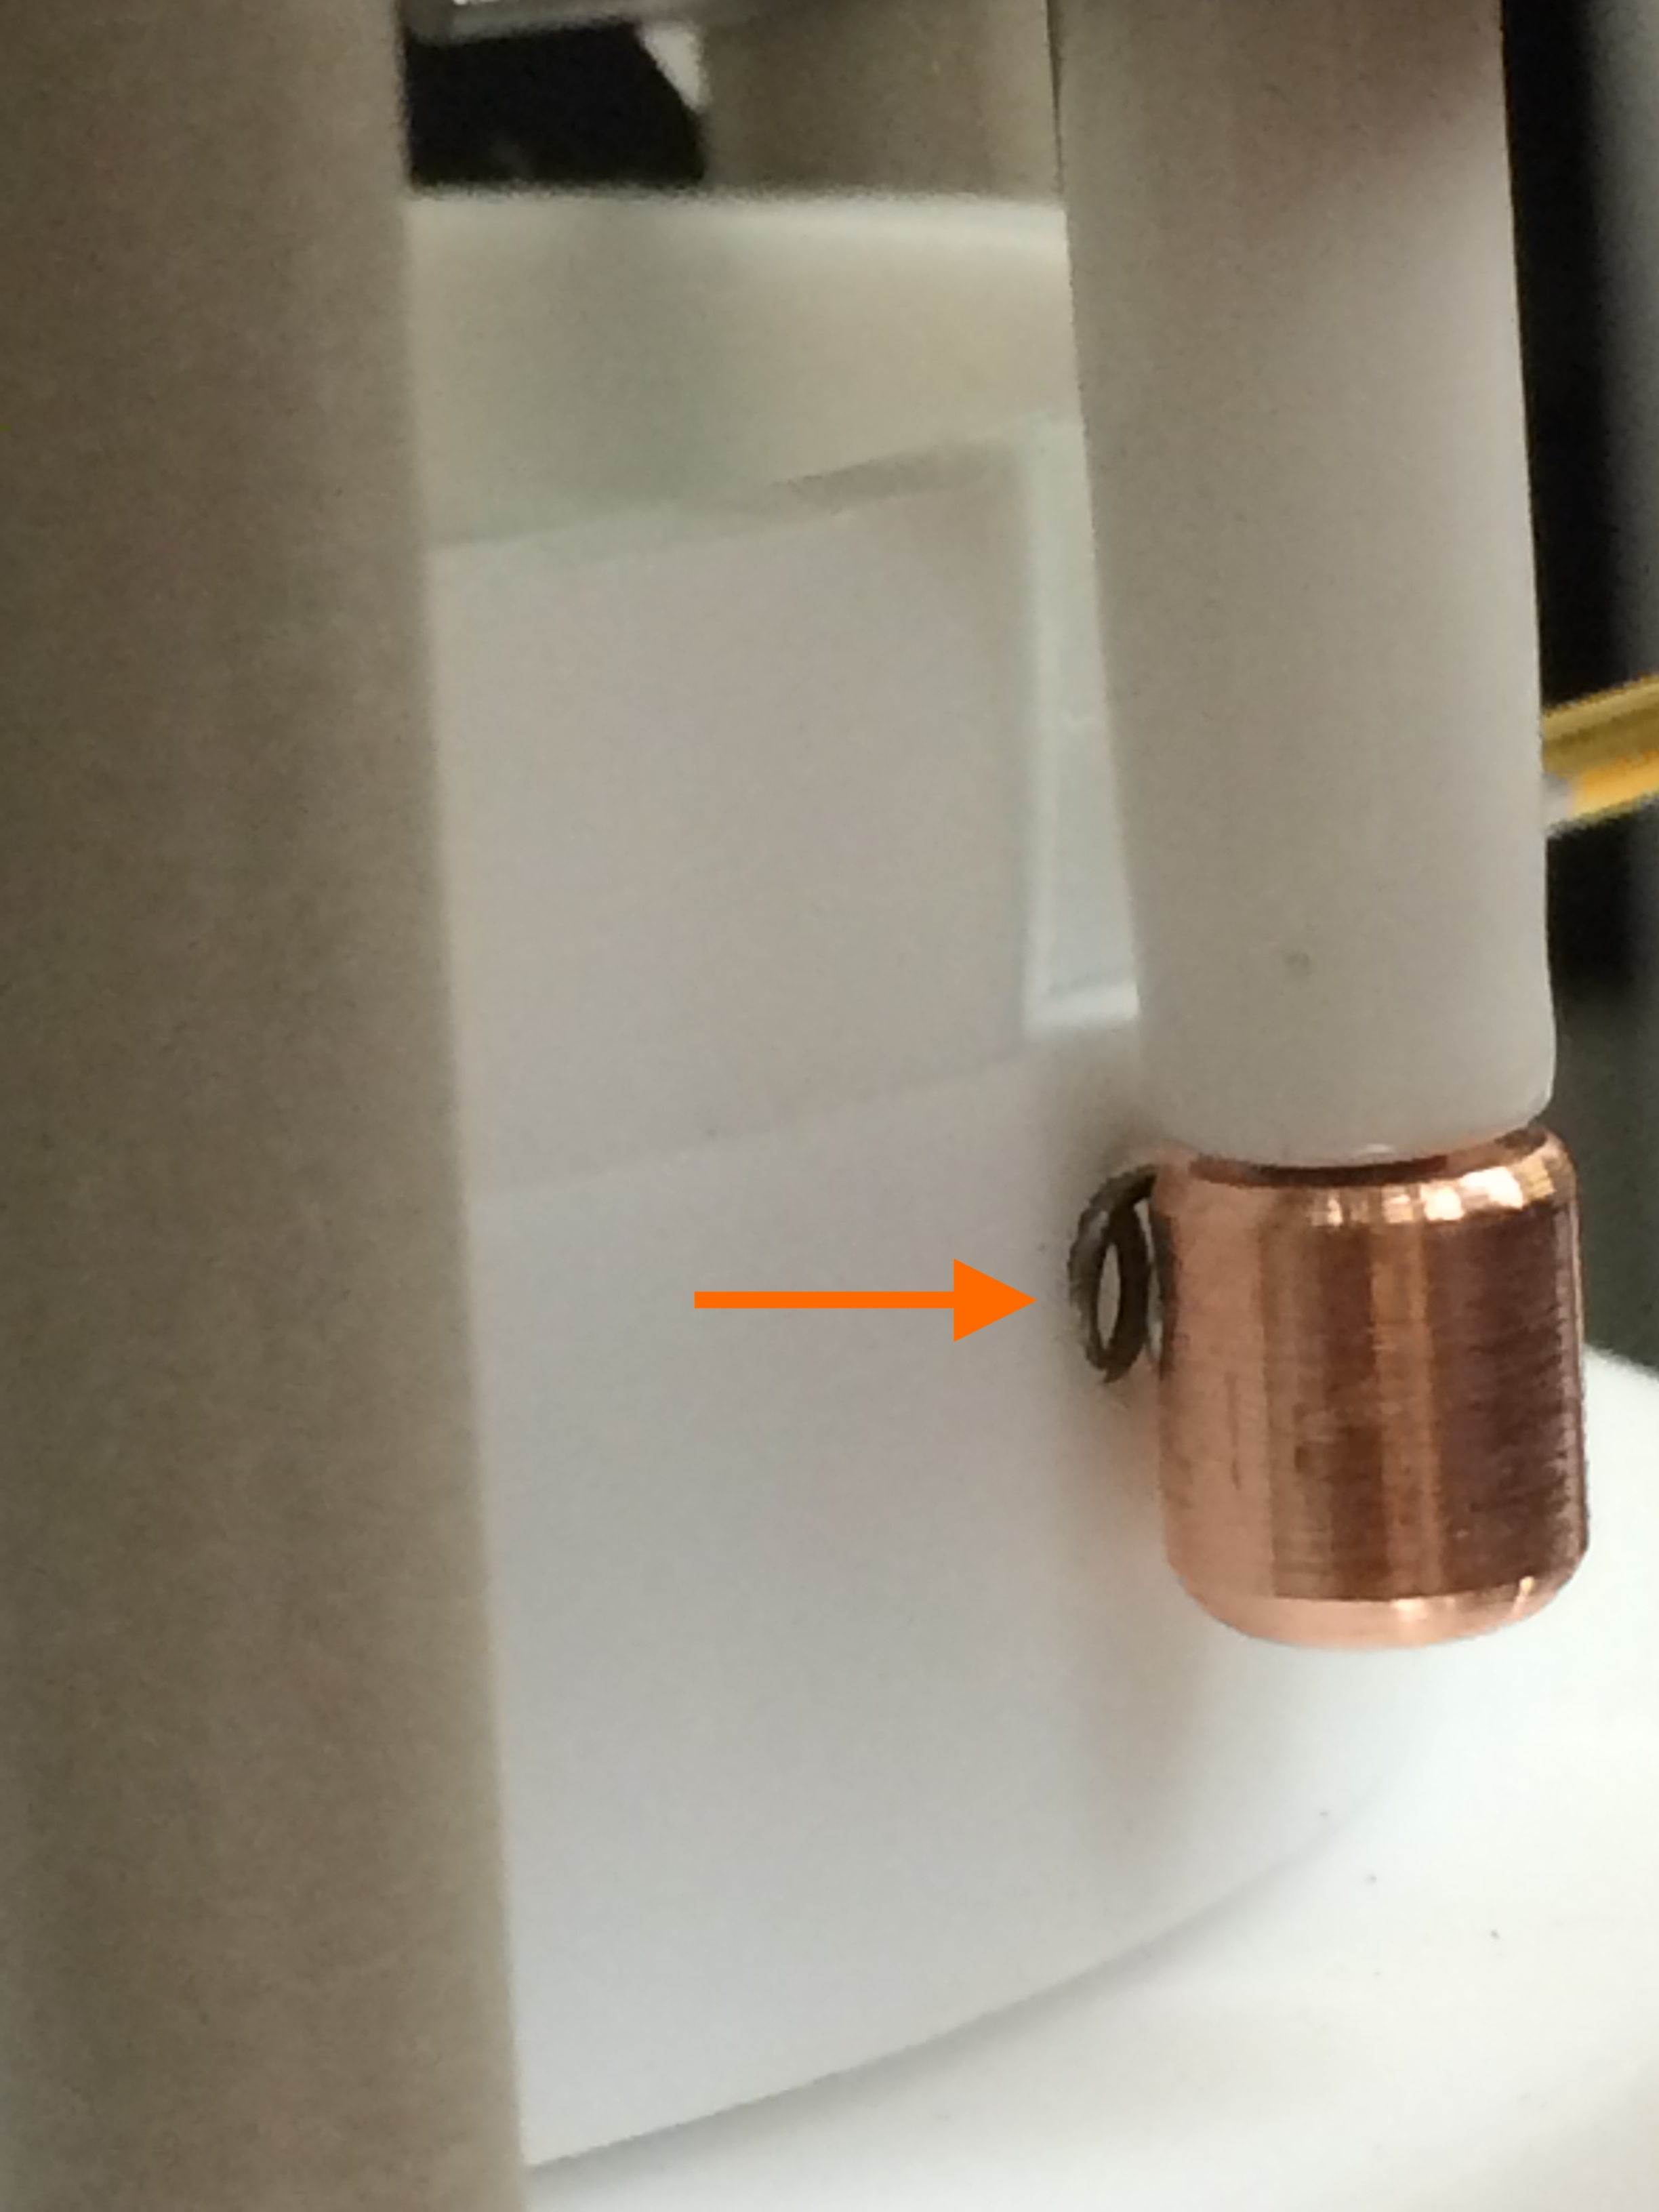
\includegraphics[width=\halffig]{figures/testbed/ft2_1.jpg}
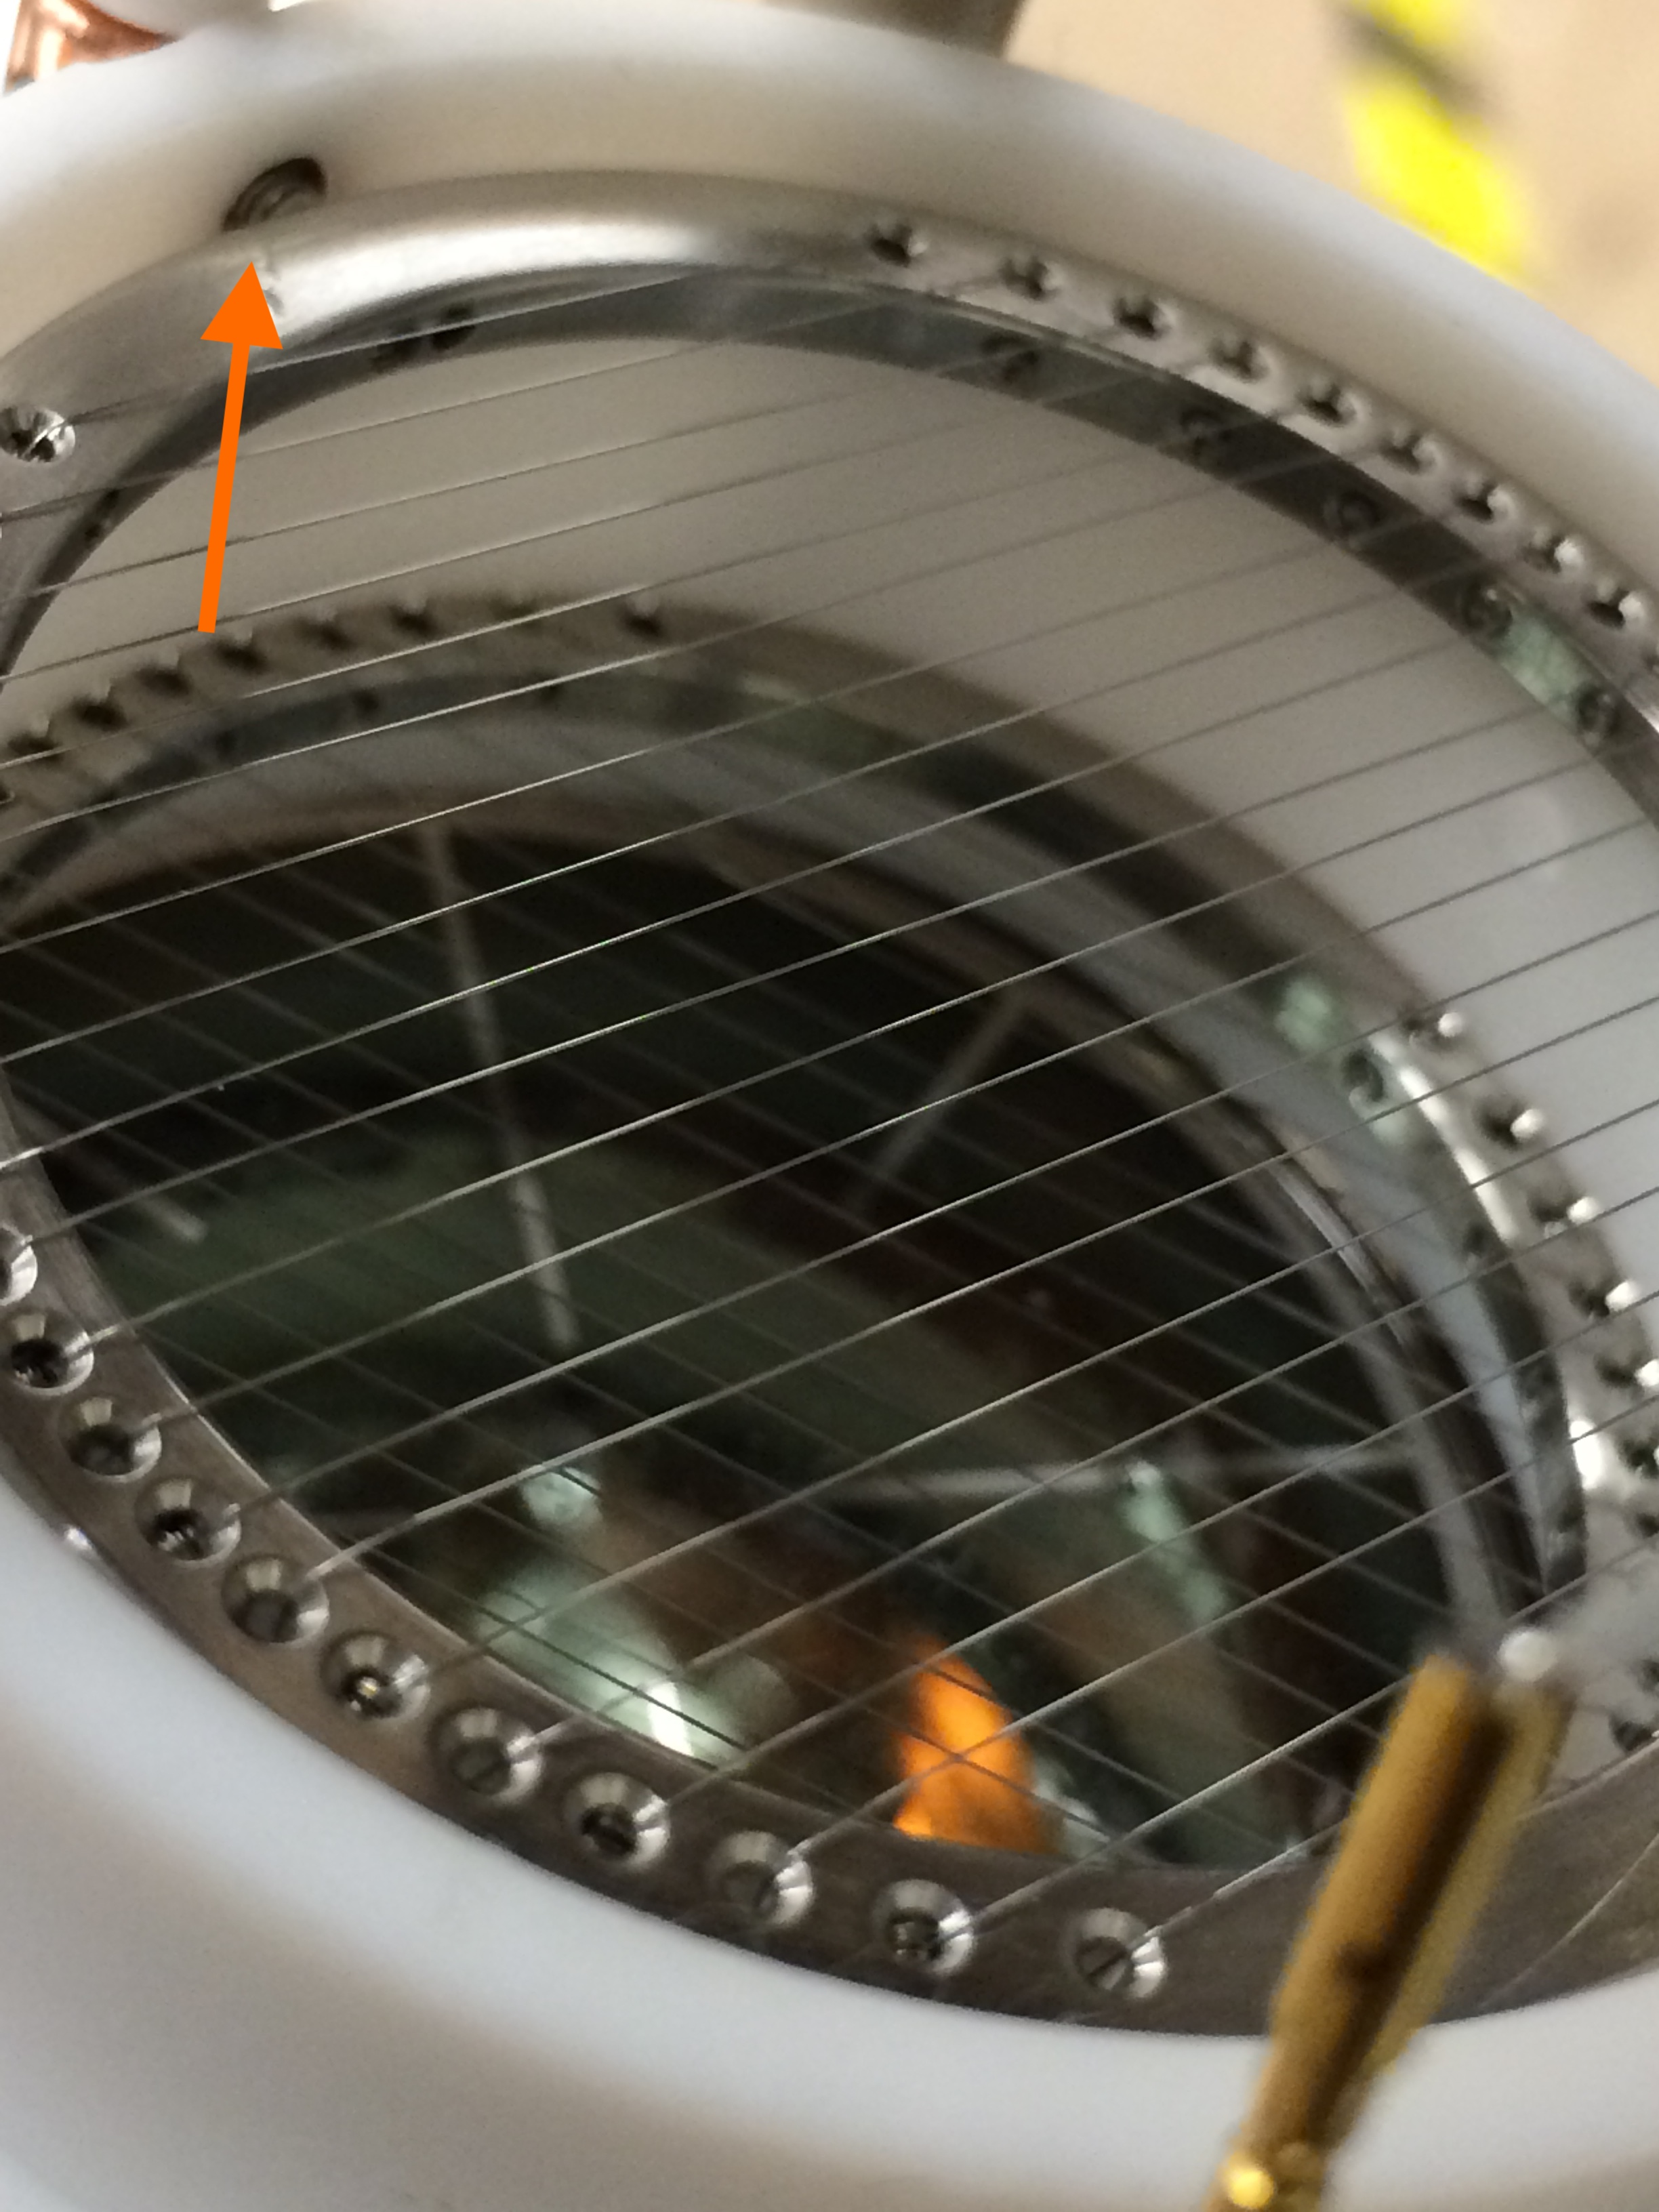
\includegraphics[width=\halffig]{figures/testbed/ft2_2.jpg}
\caption{ (left) The same 12~kV \acs{SHV} feedthrough as in Figure~\ref{fig:ft1}, now with a modified spring connection connecting the feedthrough to the grid frame. (right) A close-up of the cathode grid showing the spring connection.}
\label{fig:ft2_1}
\end{center}
\end{figure}


Feedthroughs were tested by performing a cool down, ramping the \ac{HV} supply slowly, and watching an oscilloscope for a higher than baseline photon rate (Figure~\ref{fig:phog}) or a full xenon breakdown (Figure~\ref{fig:breakdown}). The effect of raising the voltage on the \ac{HV} supply at a specific rate was also tested, and it was determined that the extremely slow and steady rate of a computer program was not necessarily superior to the imperfect method of the human experimenter. That is, the construction of the feedthrough, itself, outweighed any gains from computer-supervised voltage ramping.  


\begin{figure}[htbp]
\begin{center}
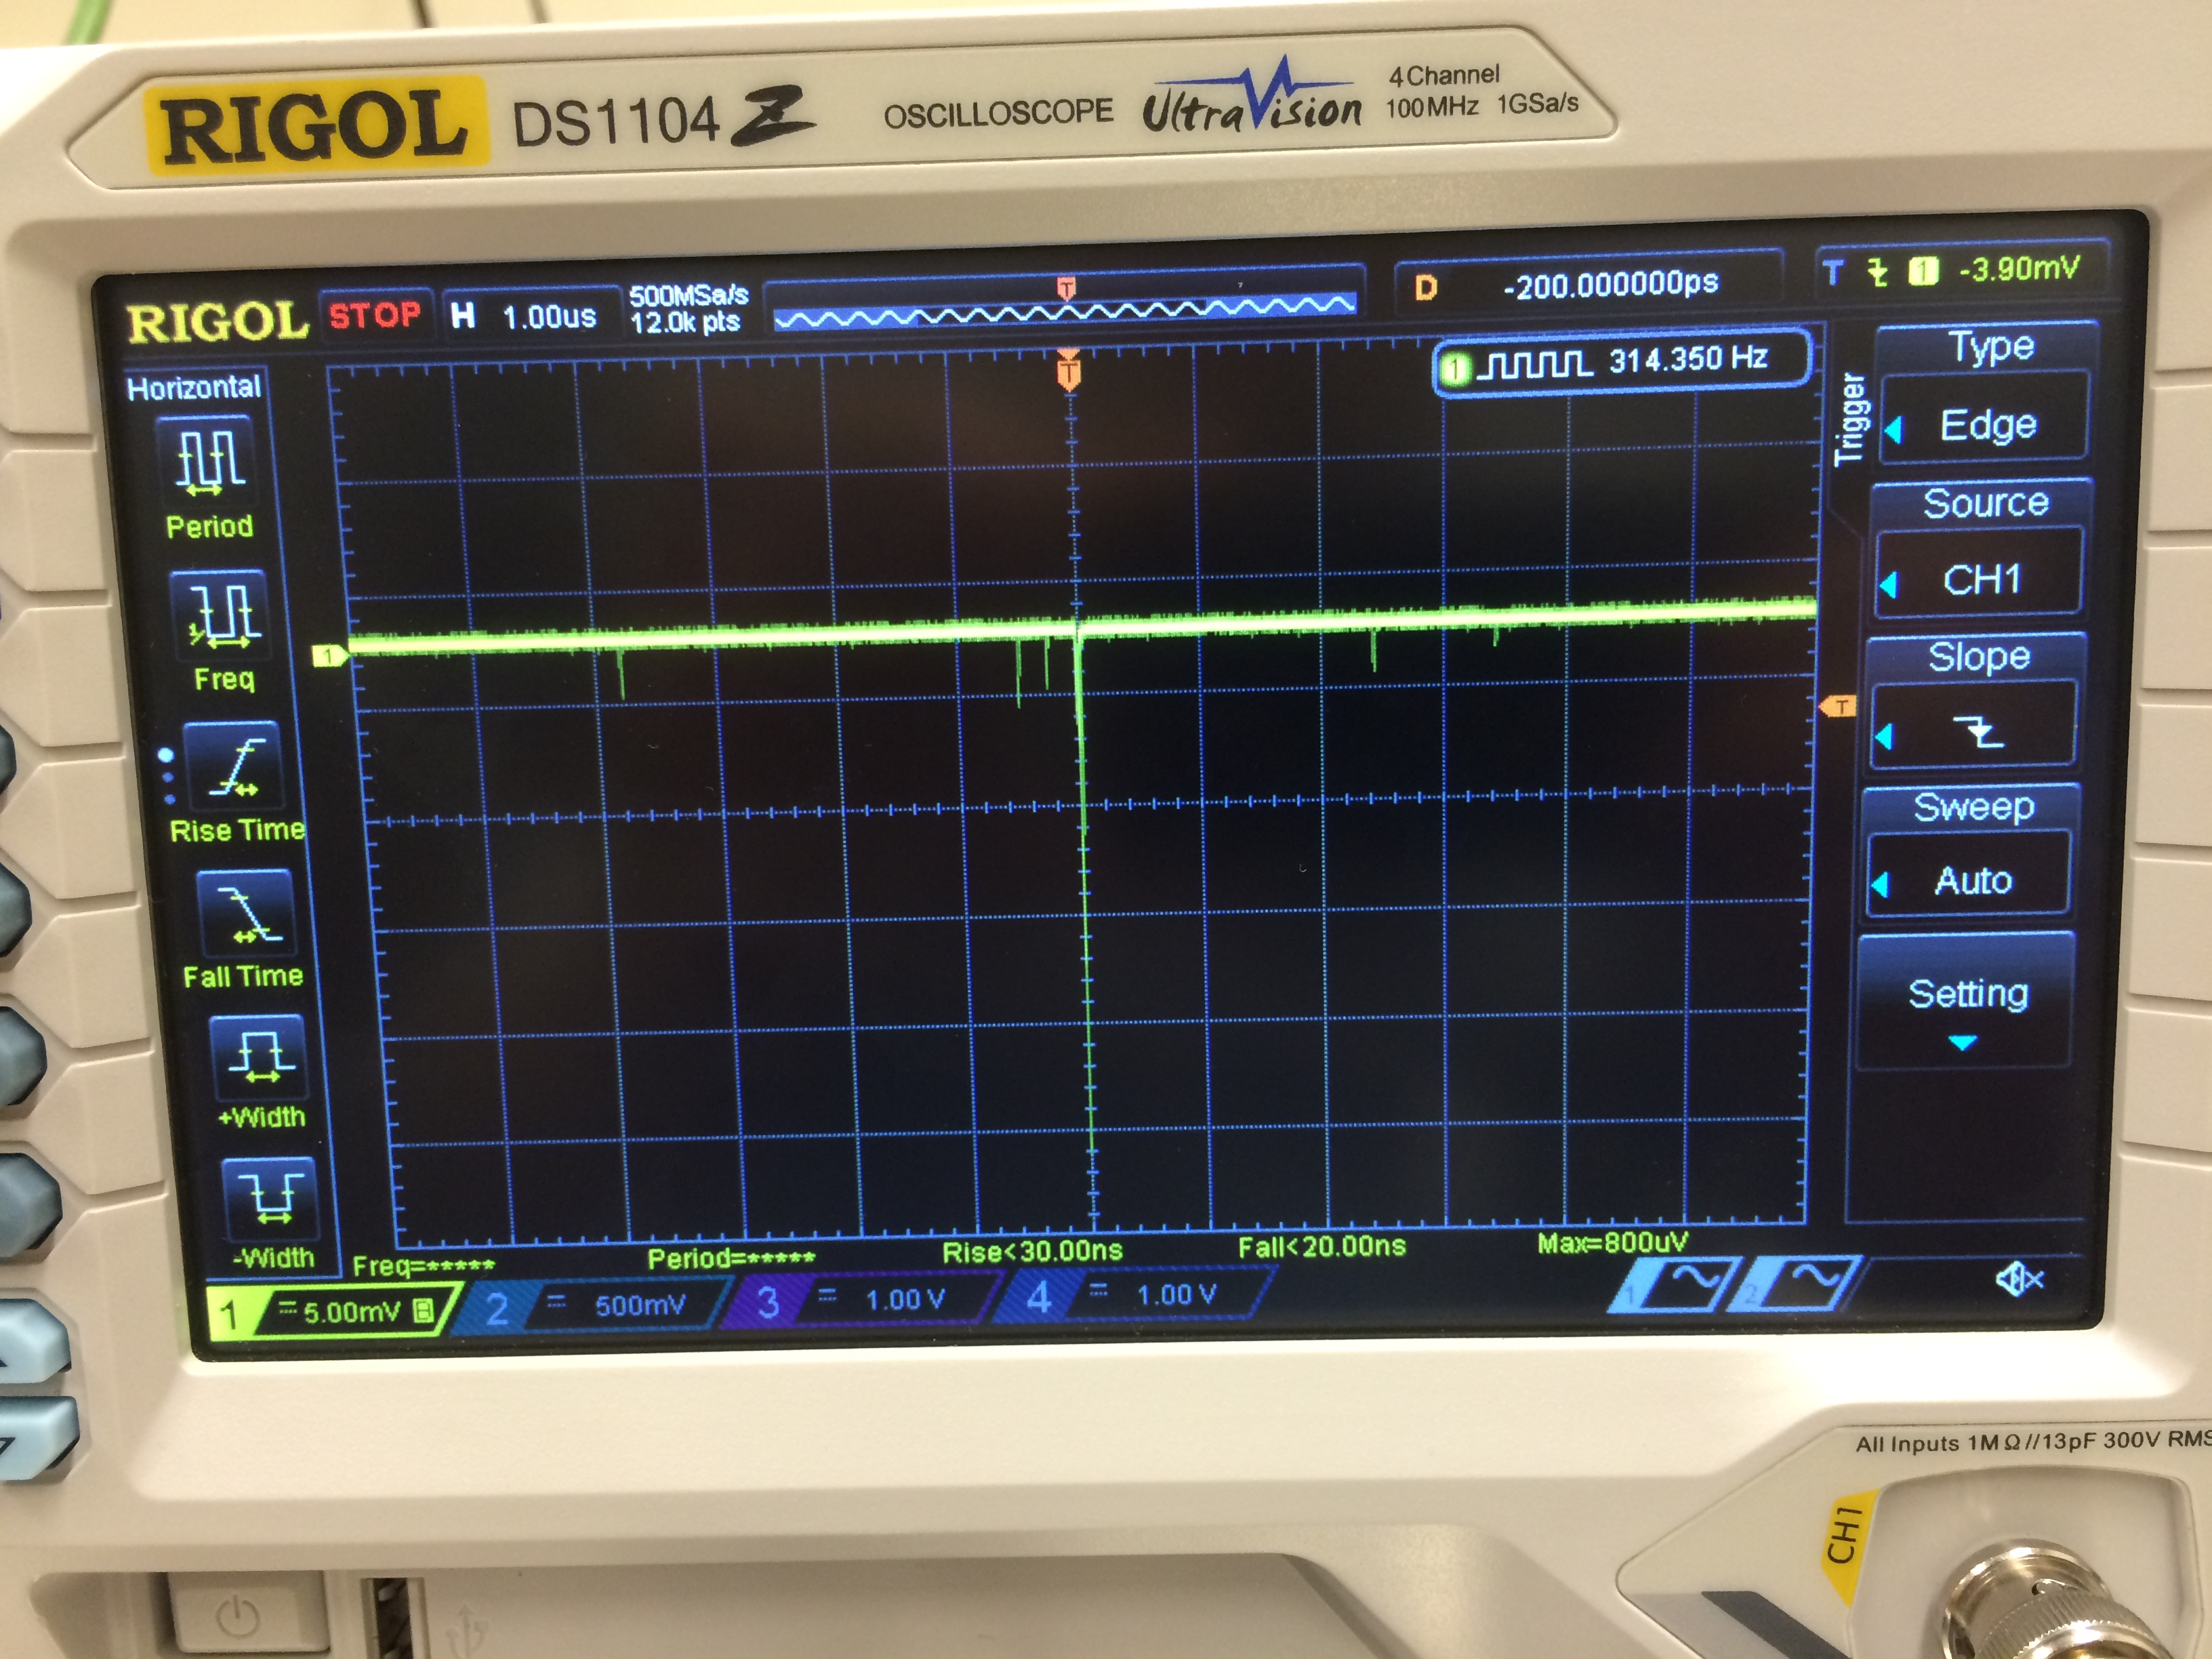
\includegraphics[width=\halffig]{figures/testbed/baseline.jpg}
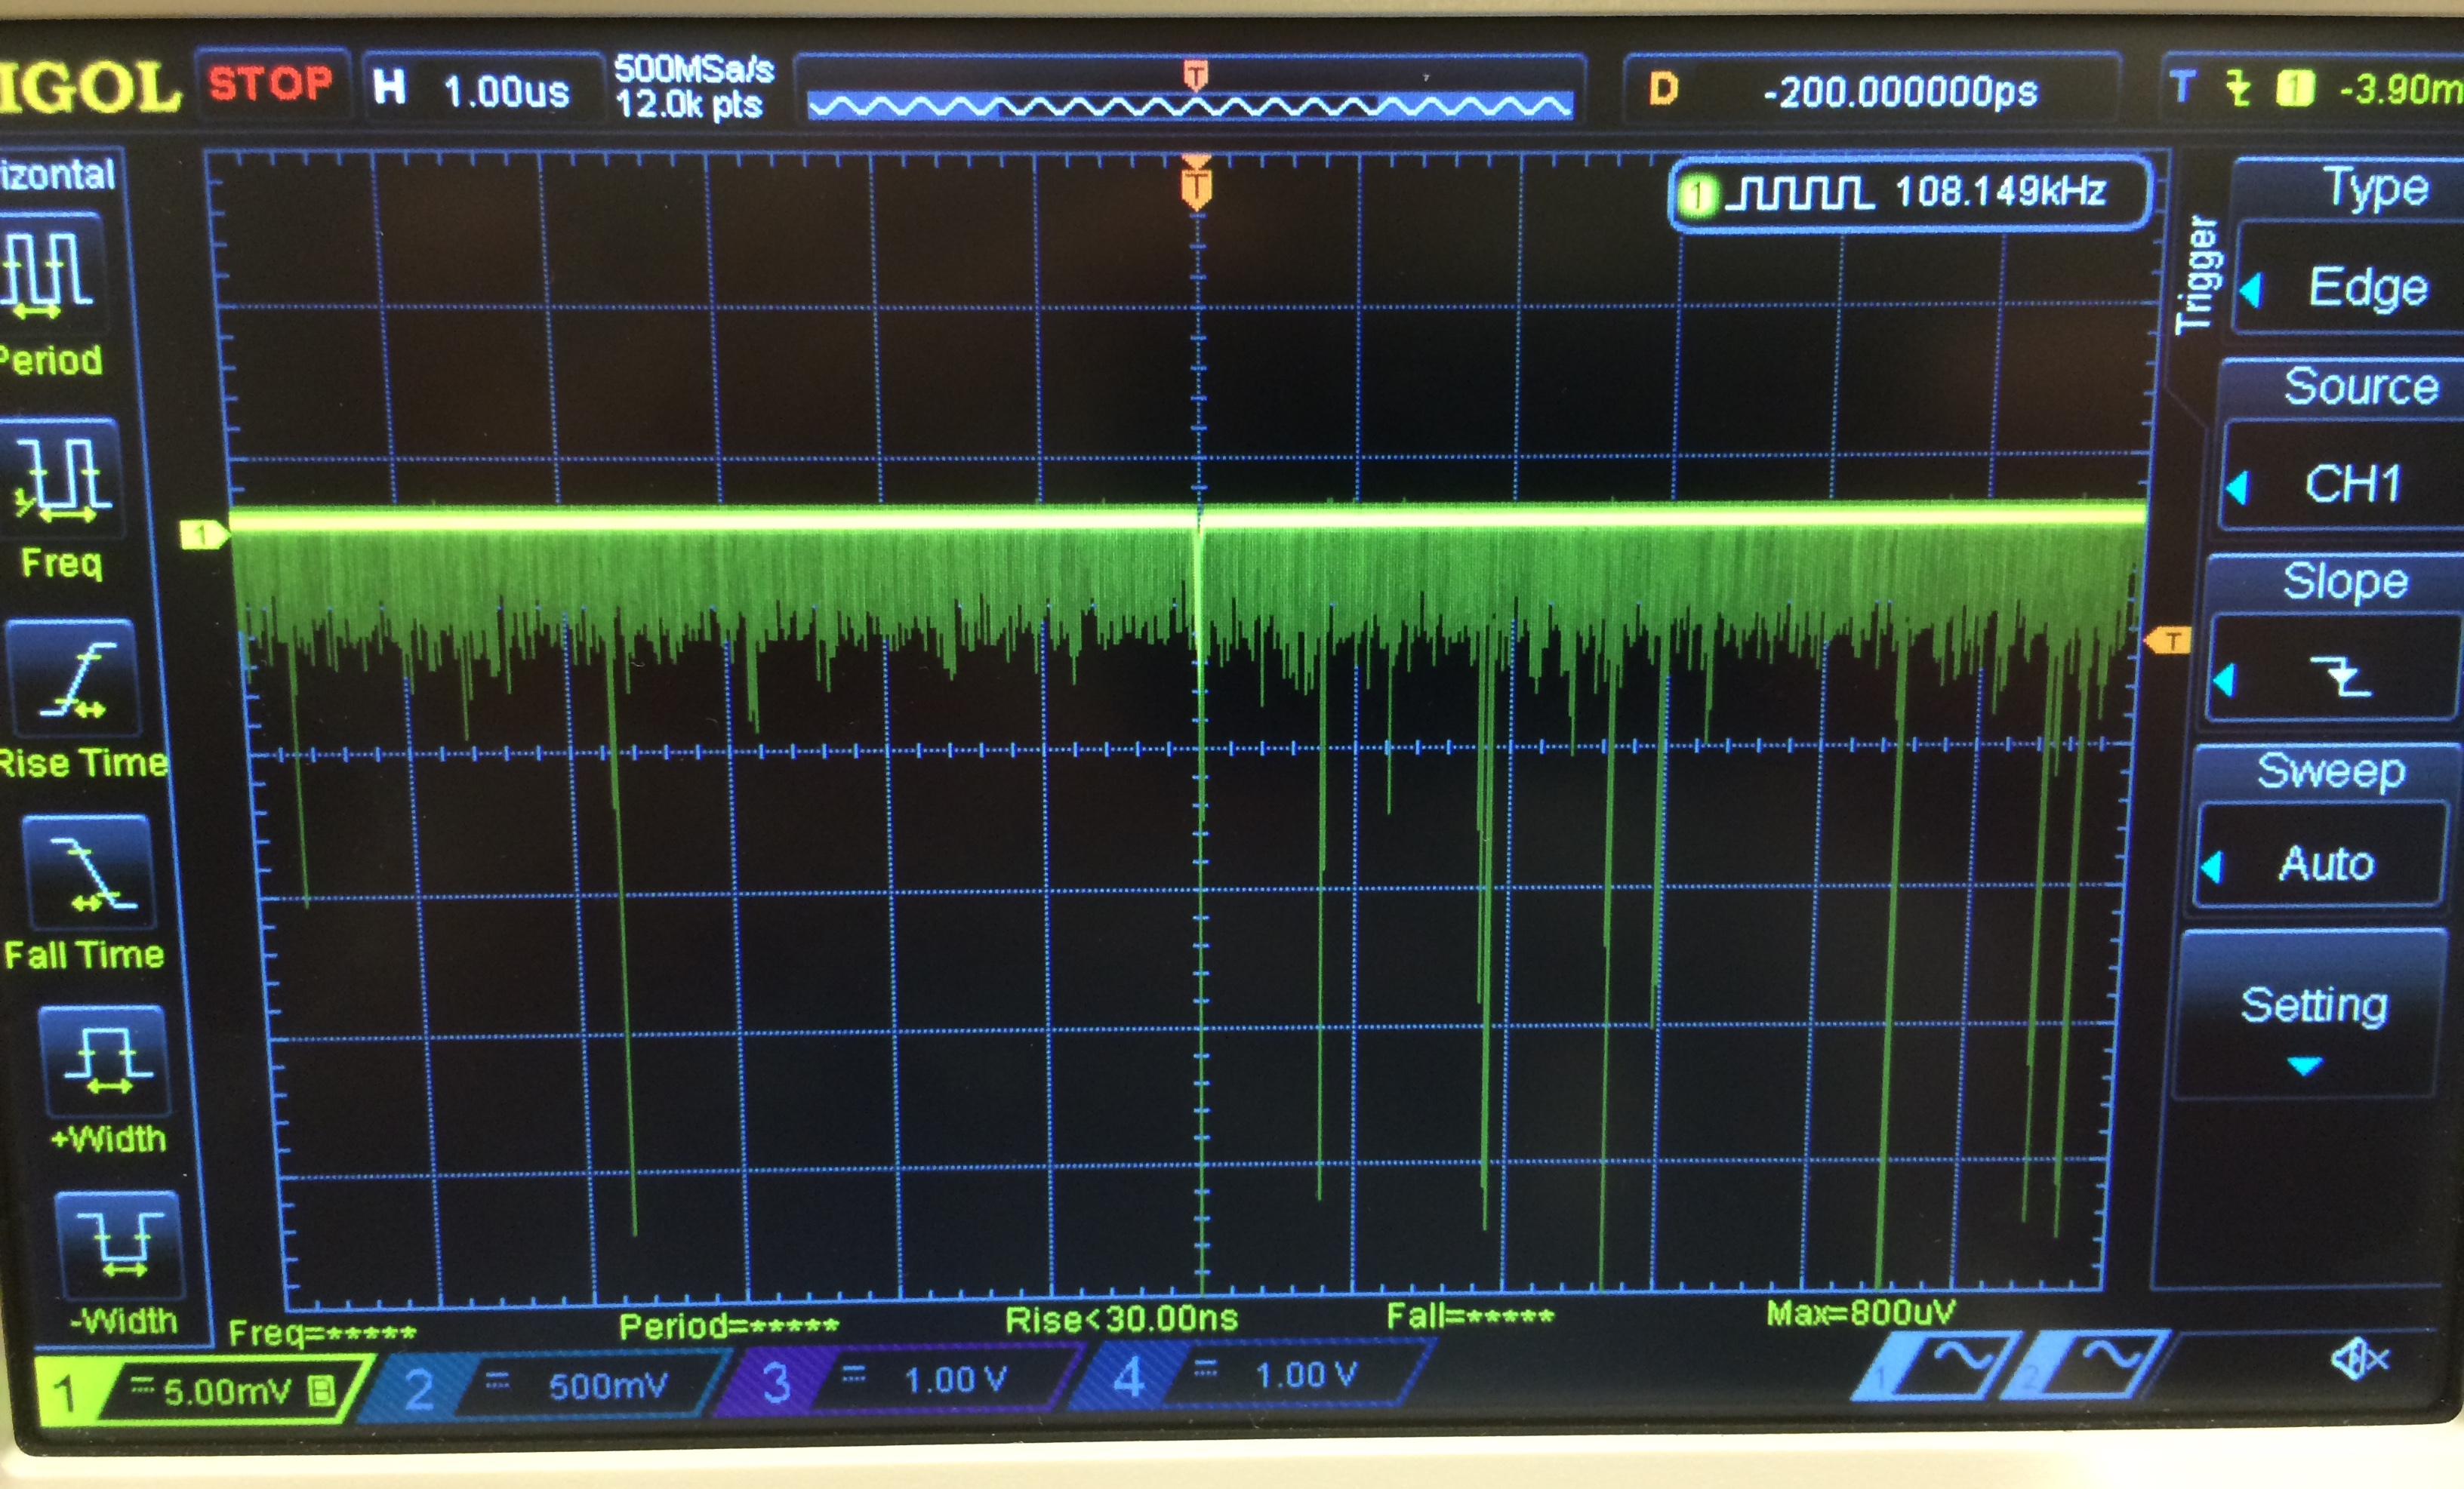
\includegraphics[width=\halffig]{figures/testbed/phog.jpg}
\caption{Oscilloscope showing baseline rate of single photons (left) compared to a high rate of single photons (right) caused by the high voltage feedthrough.}
\label{fig:phog}
\end{center}
\end{figure}


\begin{figure}[htbp]
\begin{center}
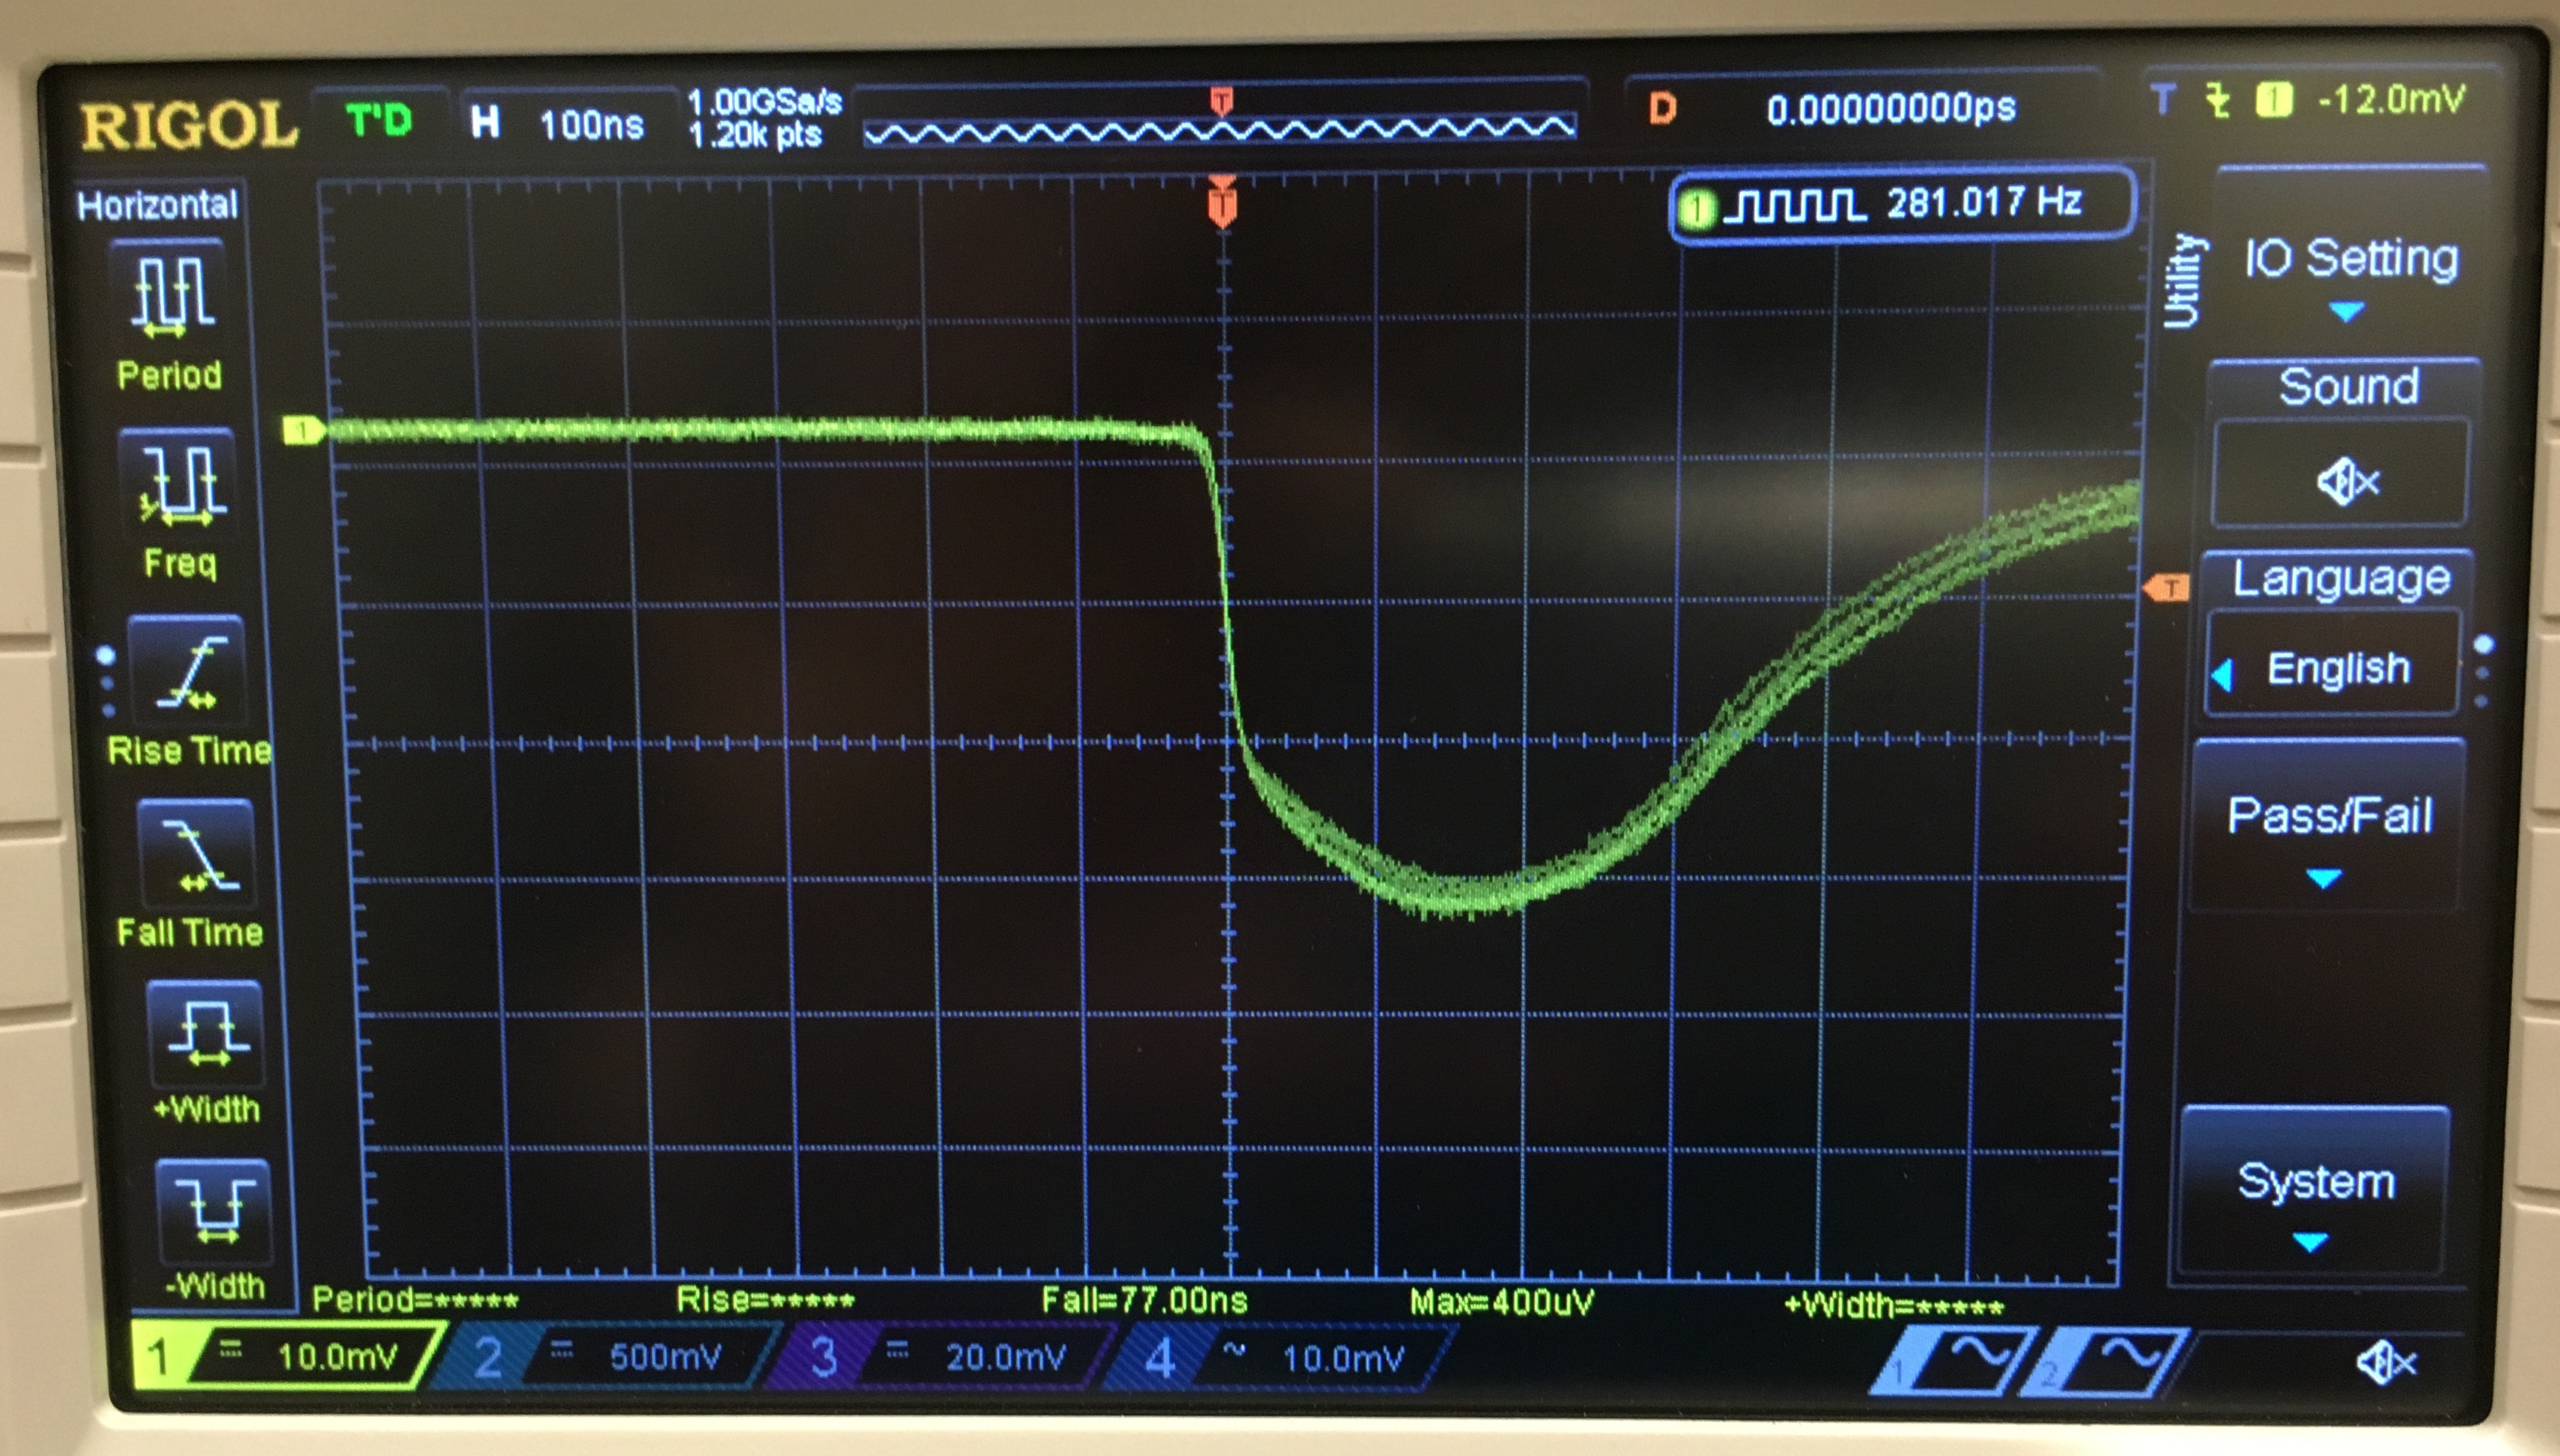
\includegraphics[width=\halffig]{figures/testbed/breakdown.jpg}
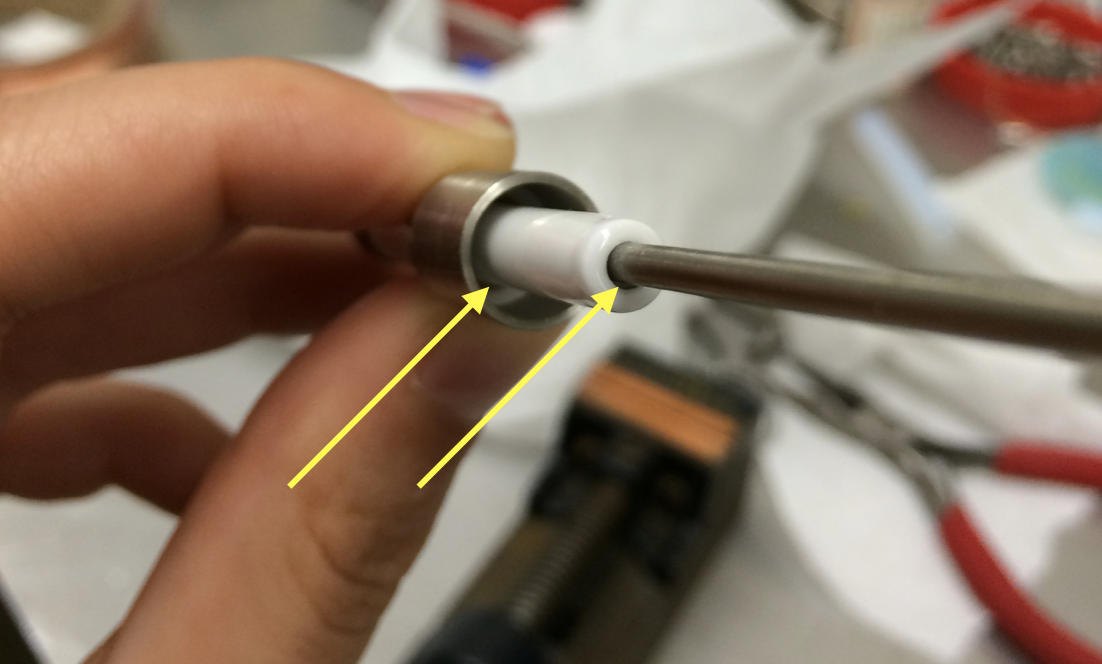
\includegraphics[width=\halffig]{figures/testbed/ft_1and2_gasgaps.png}
\caption{(left) Full xenon breakdown as visible on the \acs{PMT} trace. The large, saturated pulse is caused by the high intensity of light. This type of breakdown was often accompanied by an audible buzz, and a rise in current that would initiate a trip of the high voltage supply. (right) a close up of the xenon-facing side of the feedthrough. The arrows indicate visible gaps where xenon gas is exposed to high fields. These areas are particularly problematic for breakdowns.}
\label{fig:breakdown}
\end{center}
\end{figure}

Iterations of the 12~kV \ac{SHV} feed though were not able to reach and sustain more than about 7~kV for extended periods of time like those that would be required for data acquisition.

We also tried a stock 20~kV \ac{SHV} feedthrough with a custom end cap designed by \ac{HV} engineer Will Waldron, meant to smooth out typical triple point issues. This feedthrough was mounted on a CF flange far from the active region. A length of cable was stripped of grounding sheath for its entire length. A small section on one end was stripped of dielectric, this end was tied to the SHV feed though with copper wire, and the custom end cap was placed over this. The side of the cable making the connection to the cathode grid was drilled out for a short length on the bottom, leaving only a tube of dielectric with no conductor. A threaded rod was inserted into the cable, such that the rod made contact with the conductor. The cathode grid frame was screwed onto the threaded rod. The SHV-20 feed though is summarized in pictures in Figure~\ref{fig:shv20}, and was found to hold sufficient voltage (10~kV) for extended periods of time. It was also tested whether holding the feedthrough in place with \ac{PEEK} zip ties would increase voltage capabilities Figure~\ref{fig:zip_ties}; no change in voltage capability was observed. This feedthrough was in use for a few months, and during that time it was found that the voltage capability decreased over time; this is discussed in the next section.

\begin{figure}[htbp]
\begin{minipage}{0.43\textwidth}
    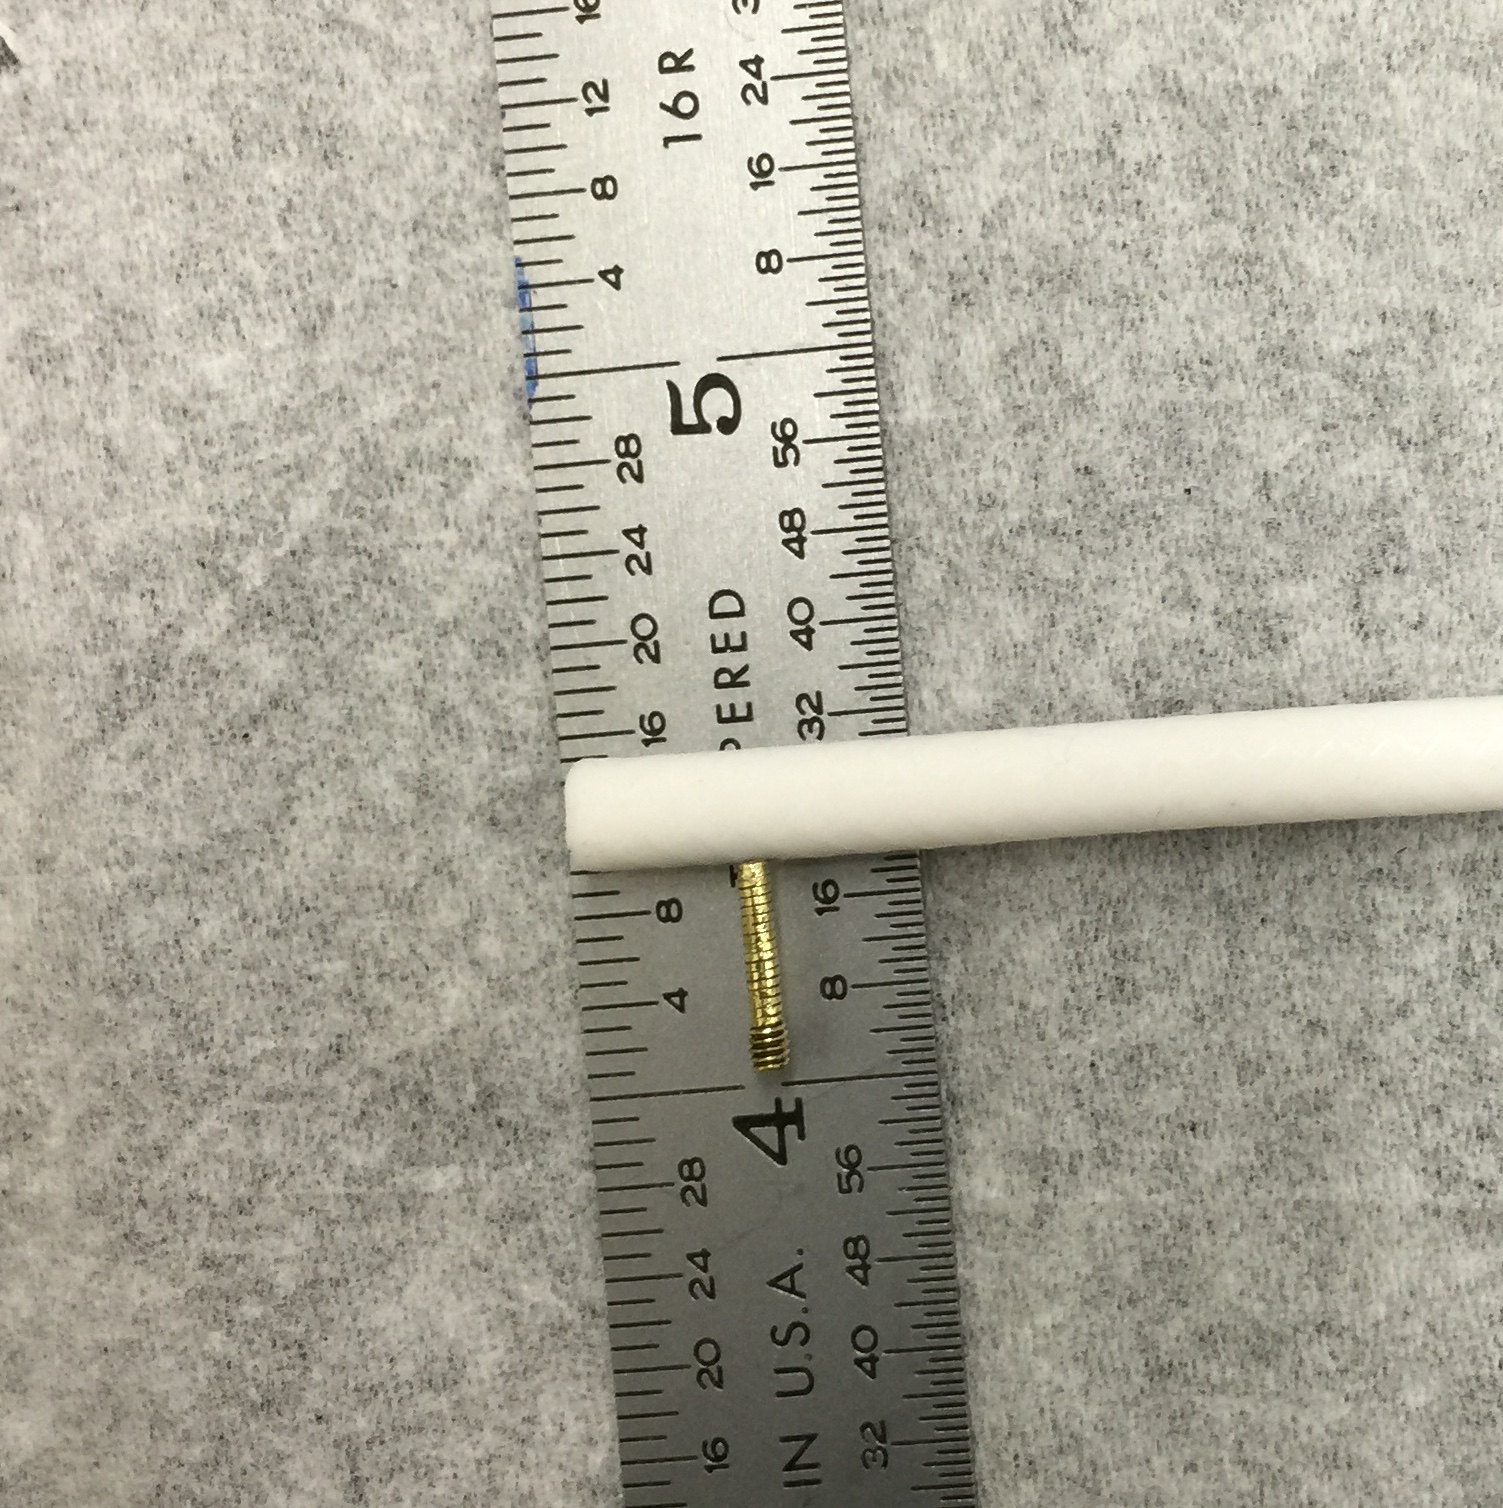
\includegraphics[width=\linewidth]{figures/testbed/ft3_1.jpg}
    \end{minipage}
    \hspace{\fill} % note: no blank line here
    \begin{minipage}{0.47\textwidth}
    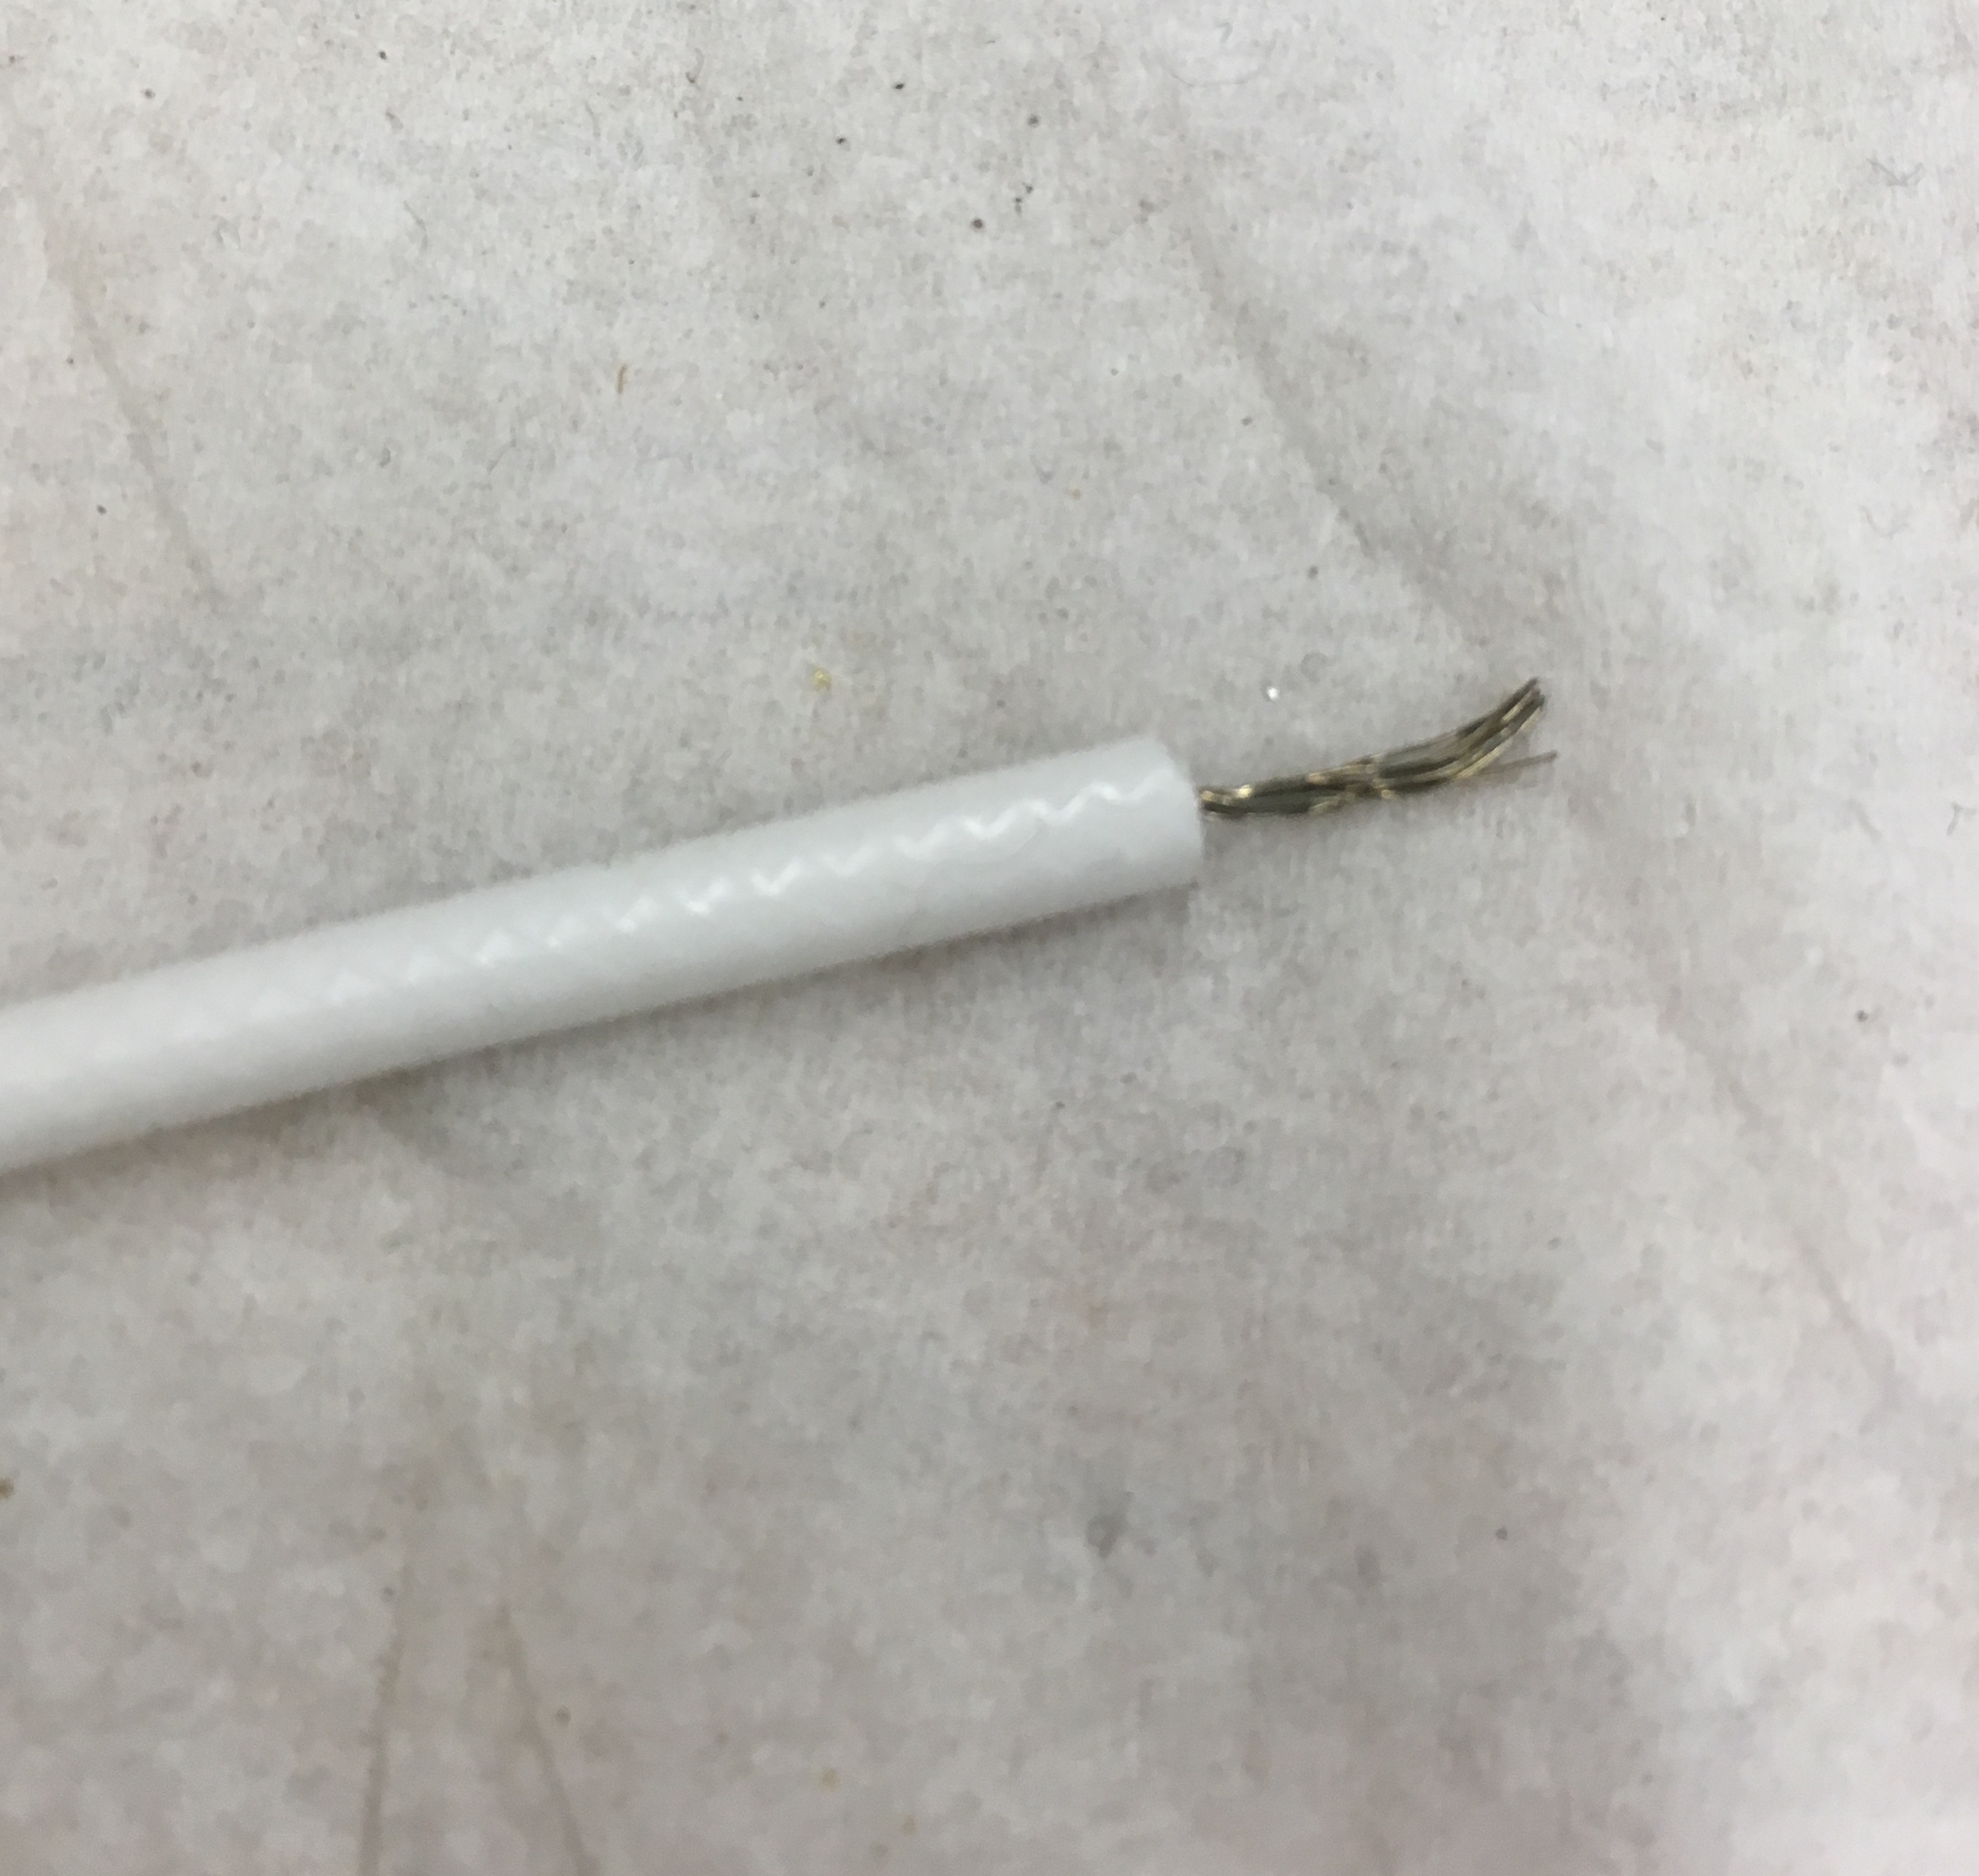
\includegraphics[width=\linewidth]{figures/testbed/ft3_2.jpg}
    \end{minipage}

    \vspace*{1cm} % vertical separation

    \begin{minipage}{0.47\textwidth}
    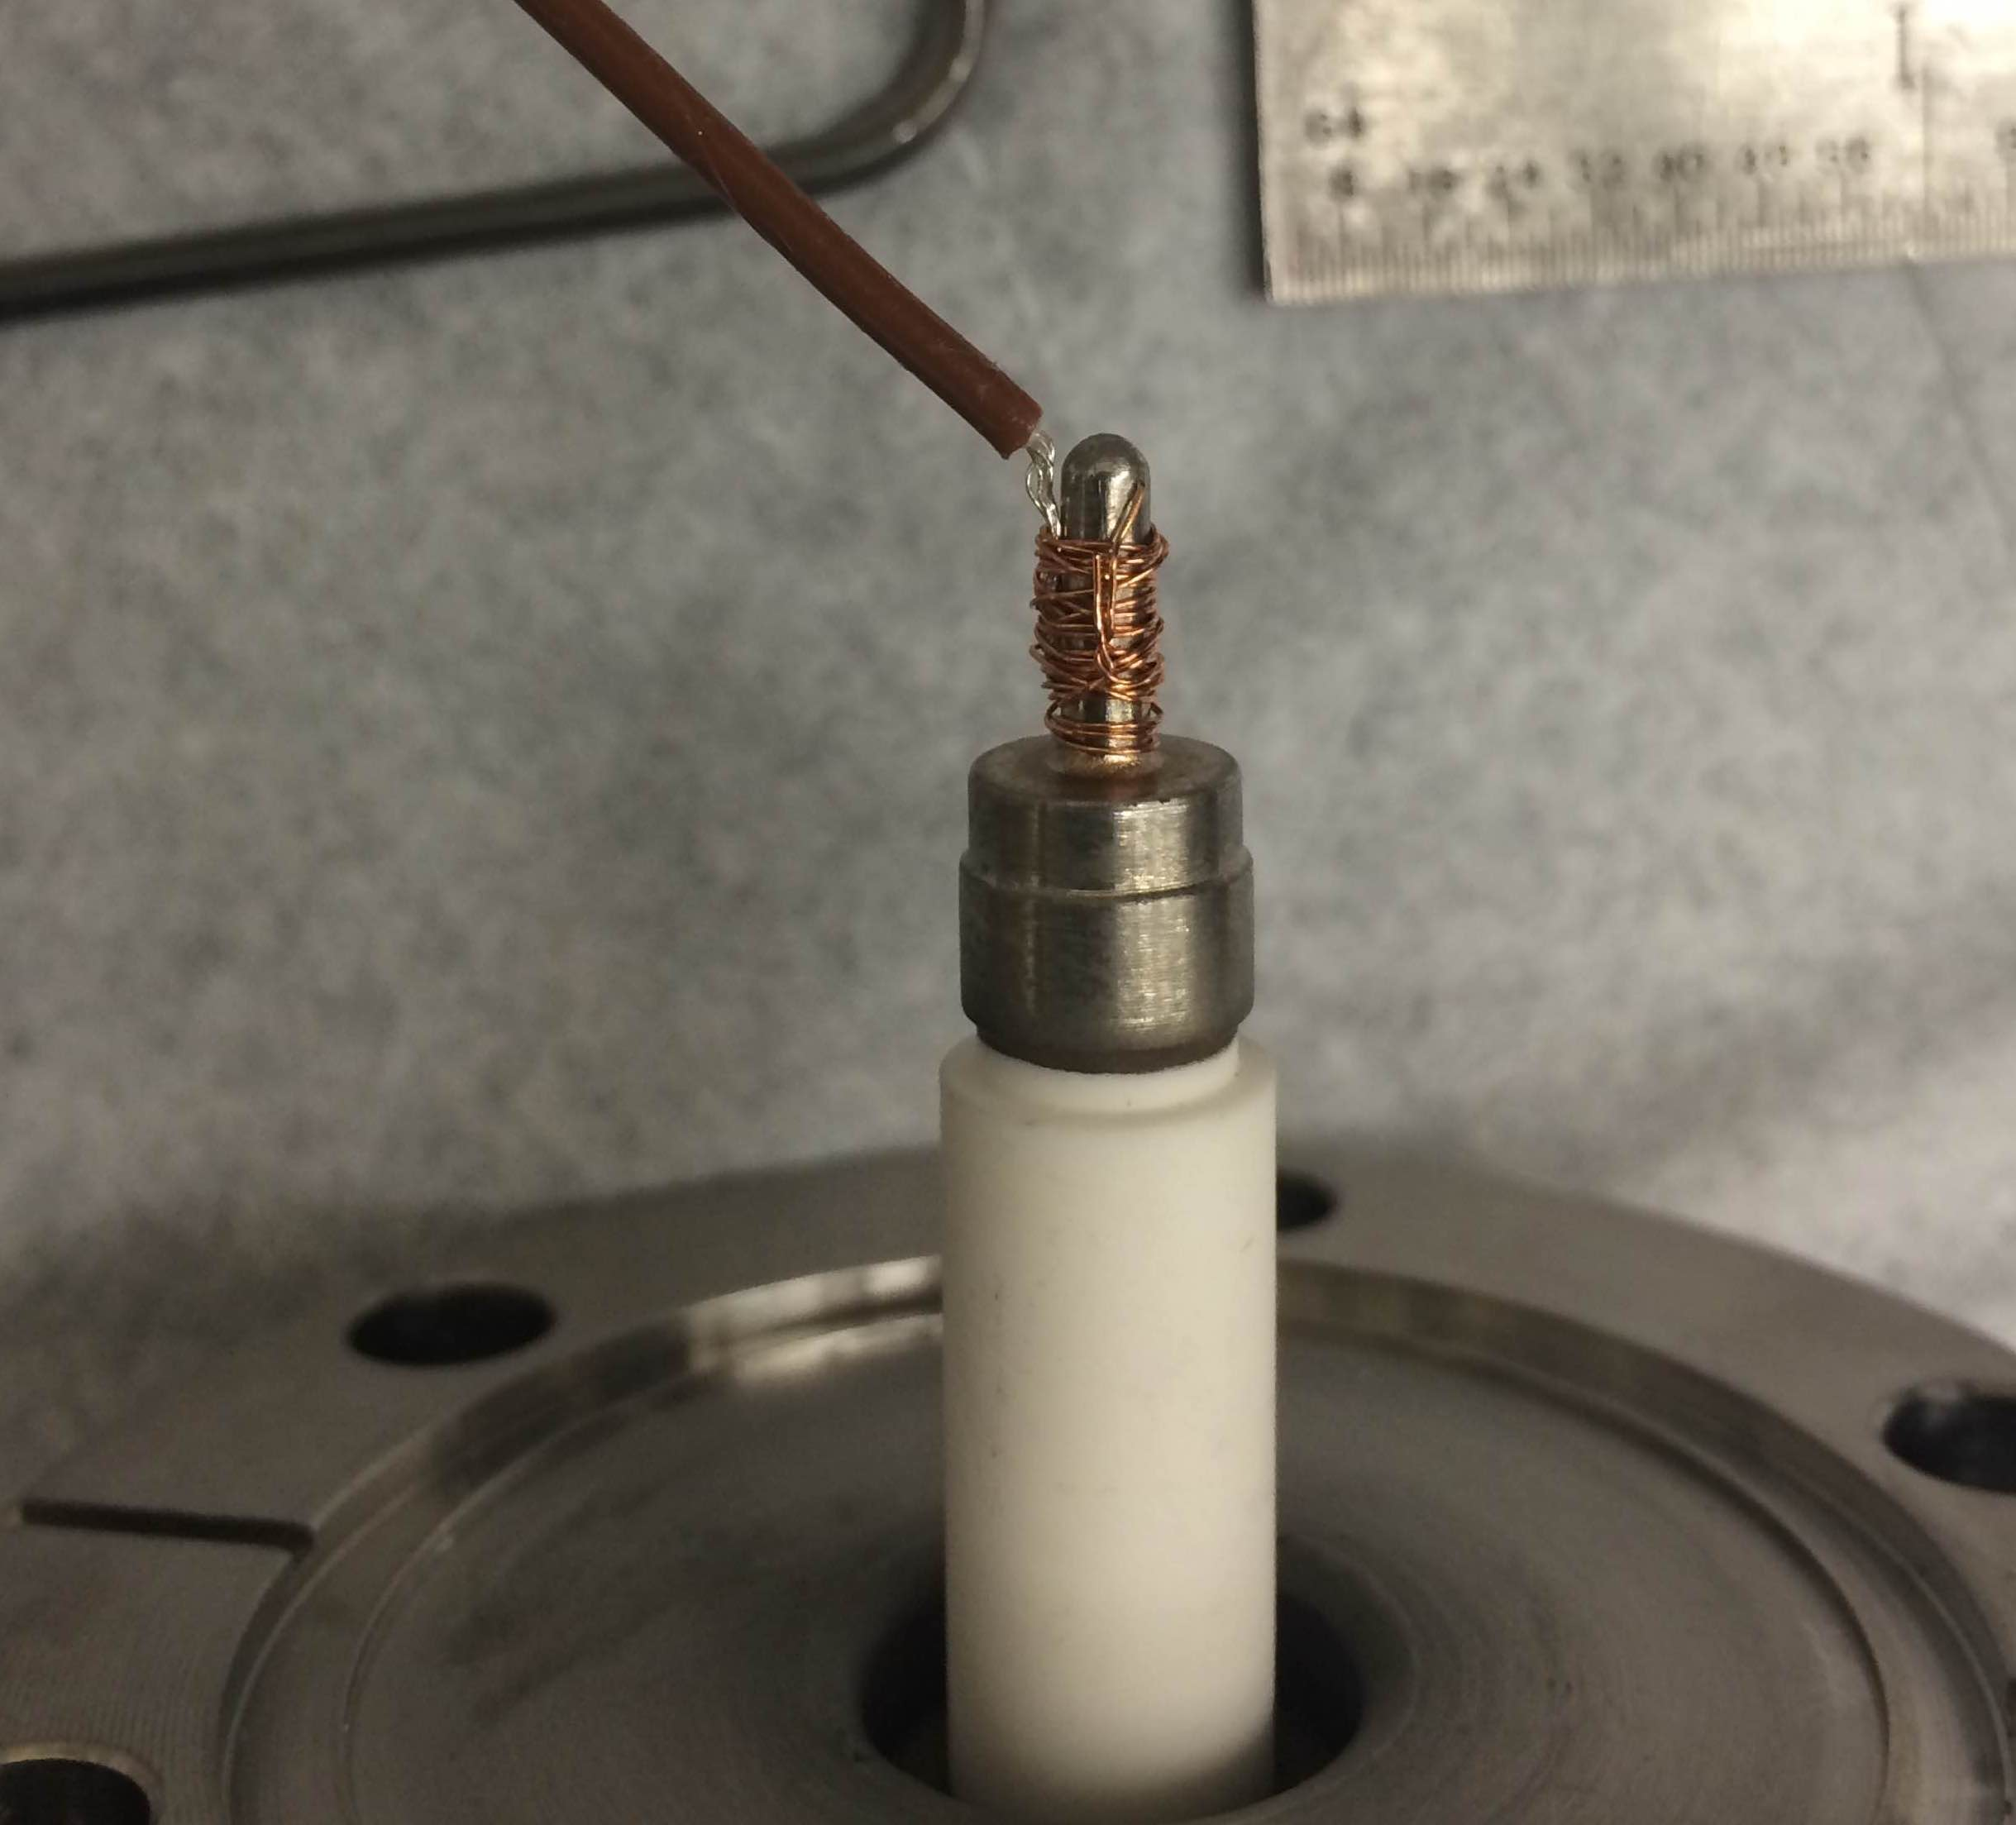
\includegraphics[width=\linewidth]{figures/testbed/ft3_3.jpg}
    \end{minipage}
    \hspace{\fill} % note: no blank line here
    \begin{minipage}{0.4\textwidth}
    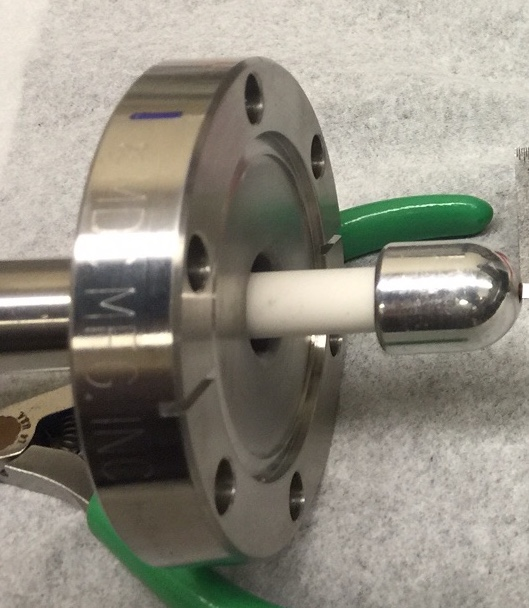
\includegraphics[width=\linewidth]{figures/testbed/ft3_4.jpg}
    \end{minipage}
\caption{Design of high voltage delivery system based on an \acs{SHV}-20 feedthrough. (top left) cathode connection side (top right) \acs{SHV}-20 connection side. (bottom left) an example showing how the cable was attached to the stock \acs{SHV}-20 feed though end (bottom right) a custom cap fit over the connection, smoothing out triple points. The cap had a hole at the tip to allow the cable to pass through.}
 \label{fig:shv20}
\end{figure}

 \begin{figure}[htbp]
\begin{center}
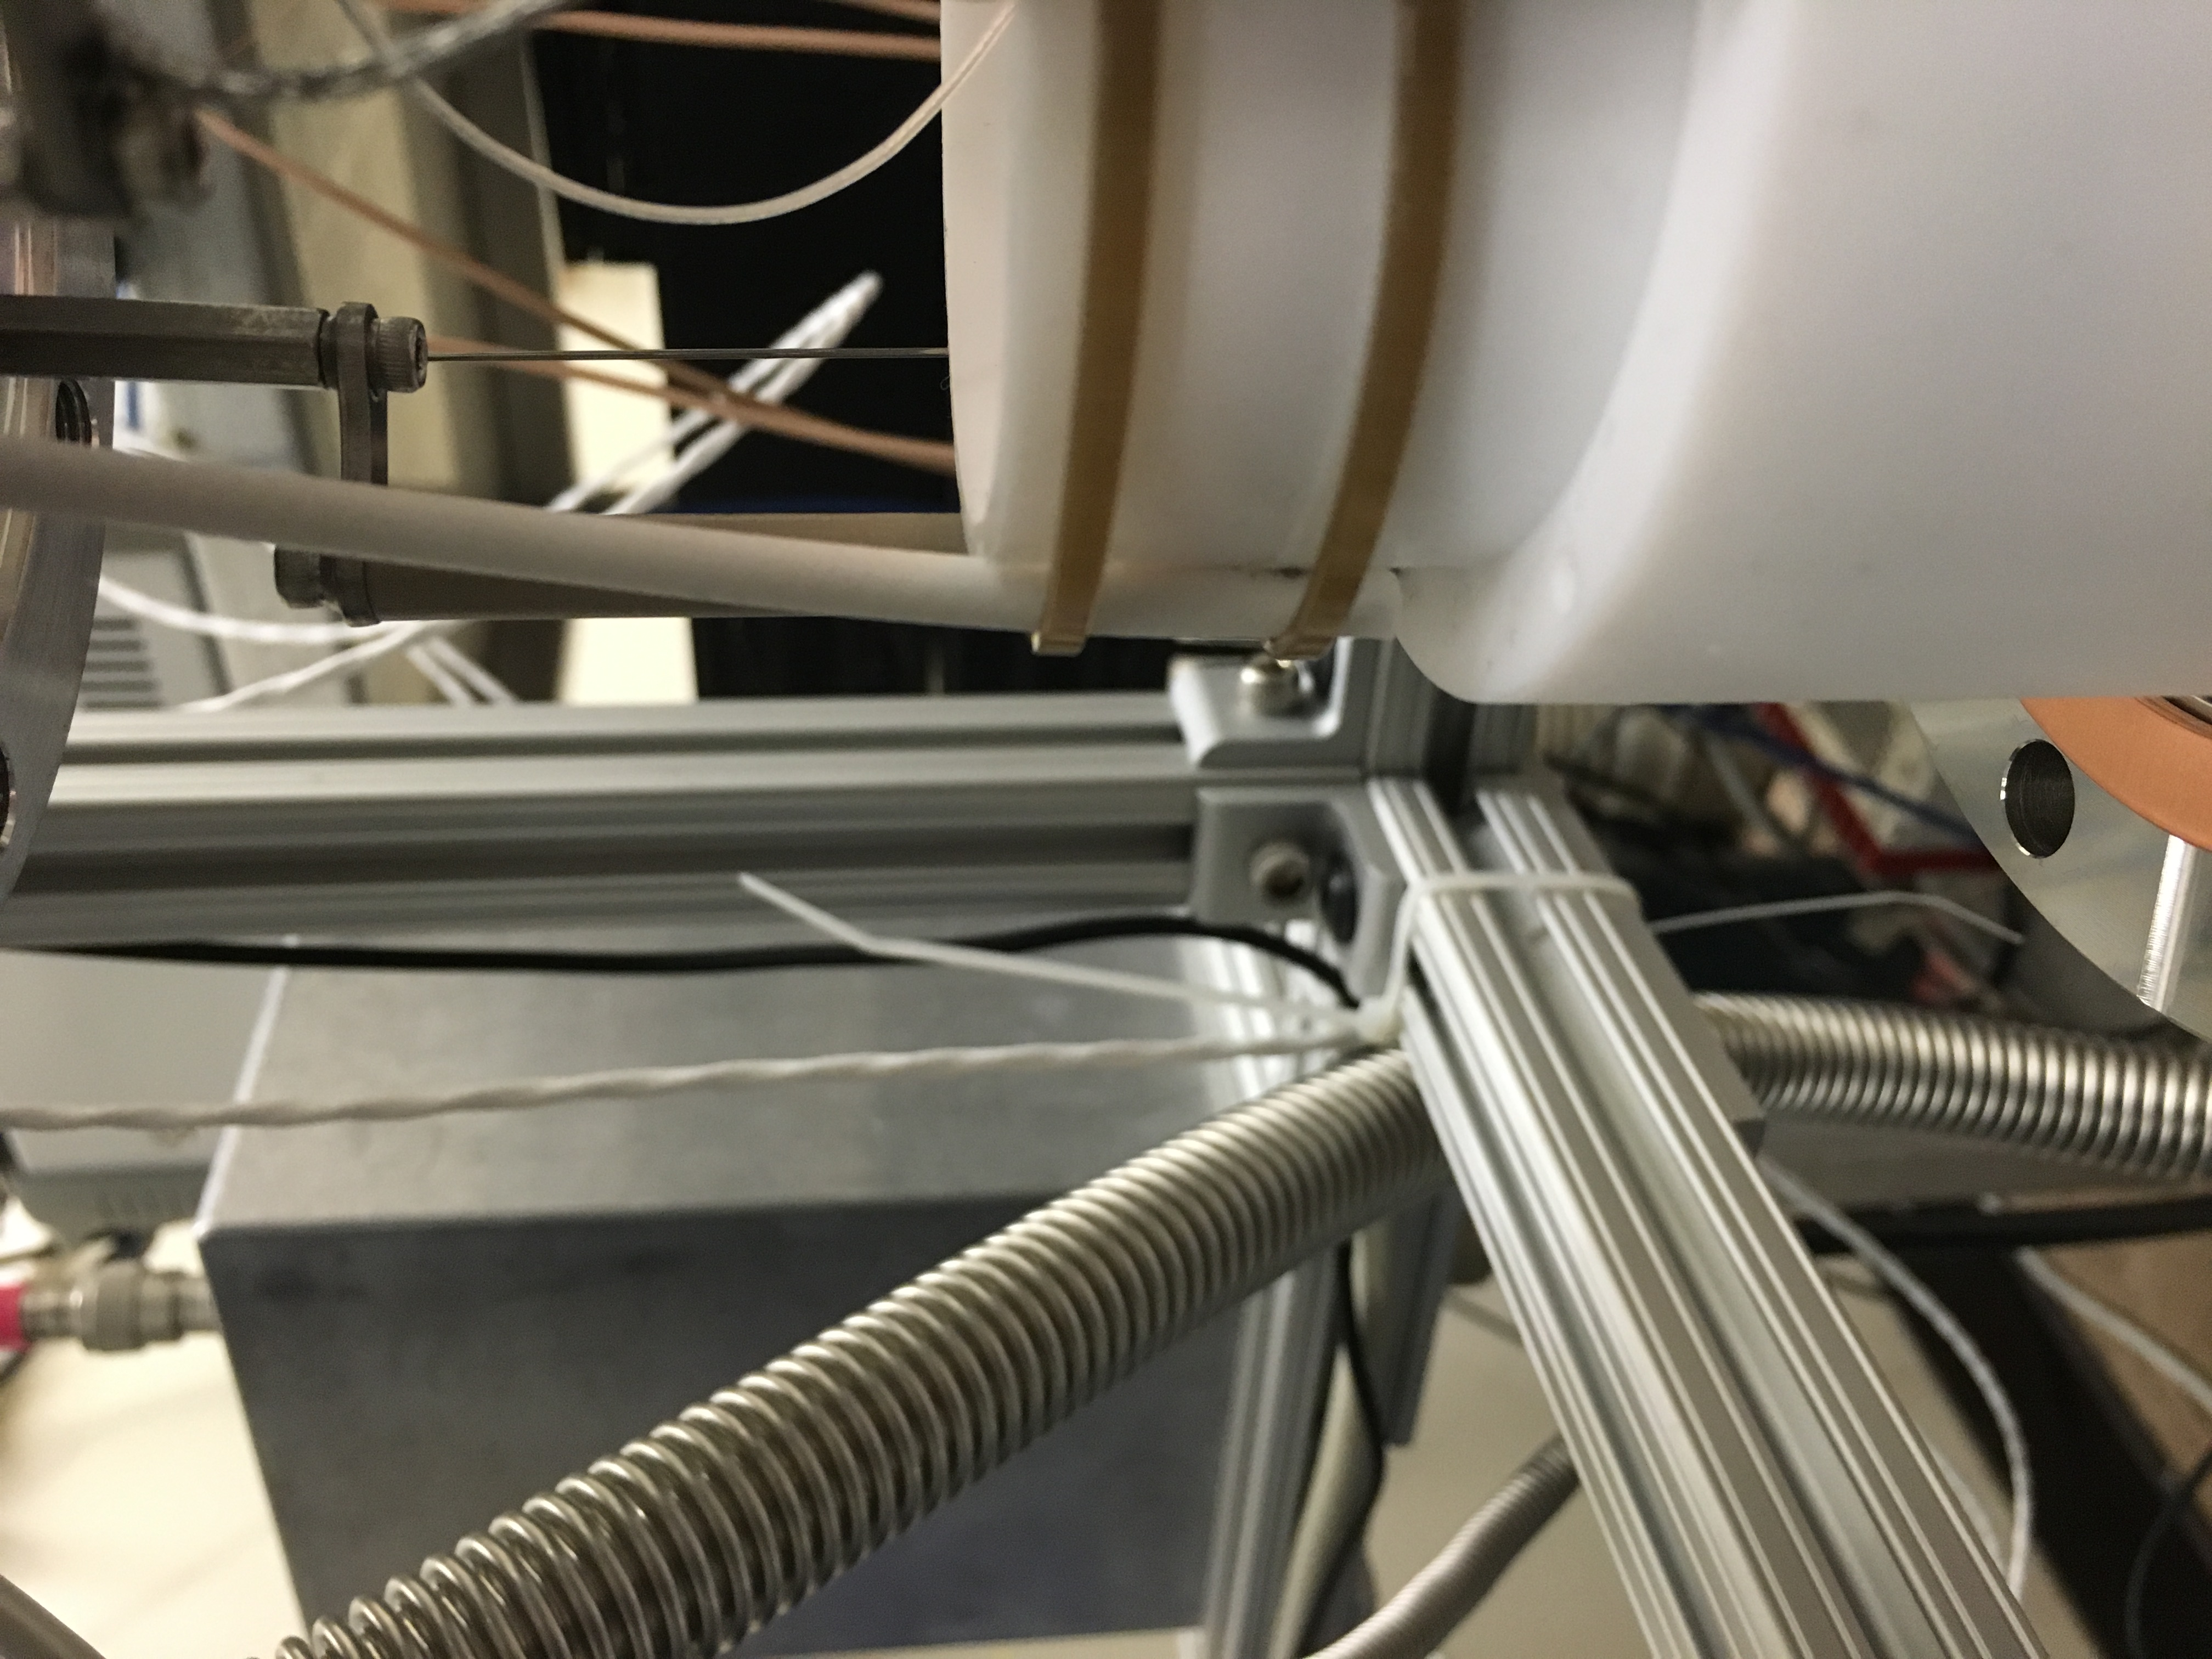
\includegraphics[width=2in, angle=-90]{figures/testbed/ft3_5.jpg}
\caption{Effect of holding the feedthrough in place with \acs{PEEK} zip ties was explored. The voltage properties were not found to improve, but neither did they degrade.}
\label{fig:zip_ties}
\end{center}
\end{figure}

% A summary of the issues with building a \ac{LXe} feedthrough out of a stock \ac{SHV} connecter is given below:
%\begin{itemize}
%\item Gas gaps
%\item Triple points
%\item Prone to aging (more in Section \ref{sec:aging})
%\end{itemize}

 \FloatBarrier
\subsubsection{Feedthrough Aging}
\label{sec:aging}
It was noticed during subsequent operation that the \ac{SHV}-20 feedthrough was subject to aging (black line in Figure~\ref{fig:aging}). A month of use resulted in noticeably lower voltage capabilities. The issue could have been at any point along the entire voltage chain: feedthrough - custom cap - connection to cable - cable - connection to grid - grid. Tests focusing on different parts of the voltage chain did not reveal any weak points. Instead, it was found that the \ac{SHV}-20 feed though, itself, was subject to aging (red line in Figure~\ref{fig:aging}). 


\begin{figure}[htbp]
\begin{center}
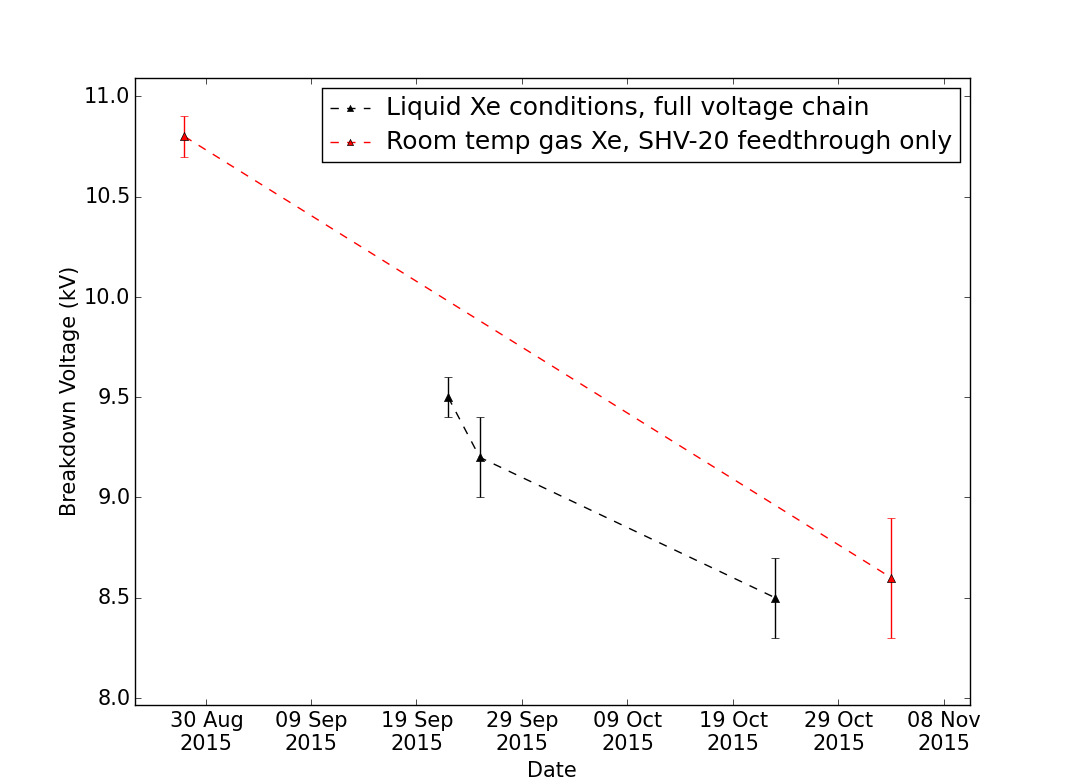
\includegraphics[width=5in]{figures/testbed/shv20_breakdowns.png}
\caption{The black line shows the aging observed in the course of normal operations. The red line shows breakdown tests of the SHV-20 feed though in gas, illustrating that the aging observed during operation was due to aging of the feed though.}
\label{fig:aging}
\end{center}
\end{figure}

Feedthrough aging can be the result of arcing and discharges which cause local heating and carbonization of an insulator surface. Once there is a carbon path, the insulator is considered ``tracked'' and then holds a much lower voltage than before. Sophisticated \ac{HV} systems keep peak currents and fault energies to a minimum using series resistors. In this way, a breakdown event does not degrade system performance in the future. In addition to carbon tracks, there can also be insulator degradation from exposure to \ac{UV} light if there is ionization in the region. Xenon ionization is in this region of the spectrum, and so any ionization near a feed though insulator may degrade the feedthrough performance. In the case of this particular feed though, the high field which caused the breakdowns or ionization was likely a result of poor triple-point geometry. 

\FloatBarrier
\subsection{Custom Feedthroughs}
To achieve better voltage performance, we moved away from typical, stock feedthroughs composed of ceramic and metal. Figure~\ref{fig:ft4} shows a feedthrough made with a Swagelock reducing union. This blue and white \ac{PTFE} piece connects 1/4~in \ac{SS} pipe to an 1/8~in \ac{PTFE} tube, which then houses a \ac{SS} rod. The rod is screwed onto a connector, which holds a wire to connect to the grid. This feedthrough had stable voltage performance, but could not achieve sustained voltages higher than about 9~kV. A woven \ac{SS} shield was added to the feed though to reach higher voltages (Figure~\ref{fig:ft4} (left)) but this actually decreased the voltage performance to a maximum of about 5~kV.   

\begin{figure}[htbp]
\begin{center}
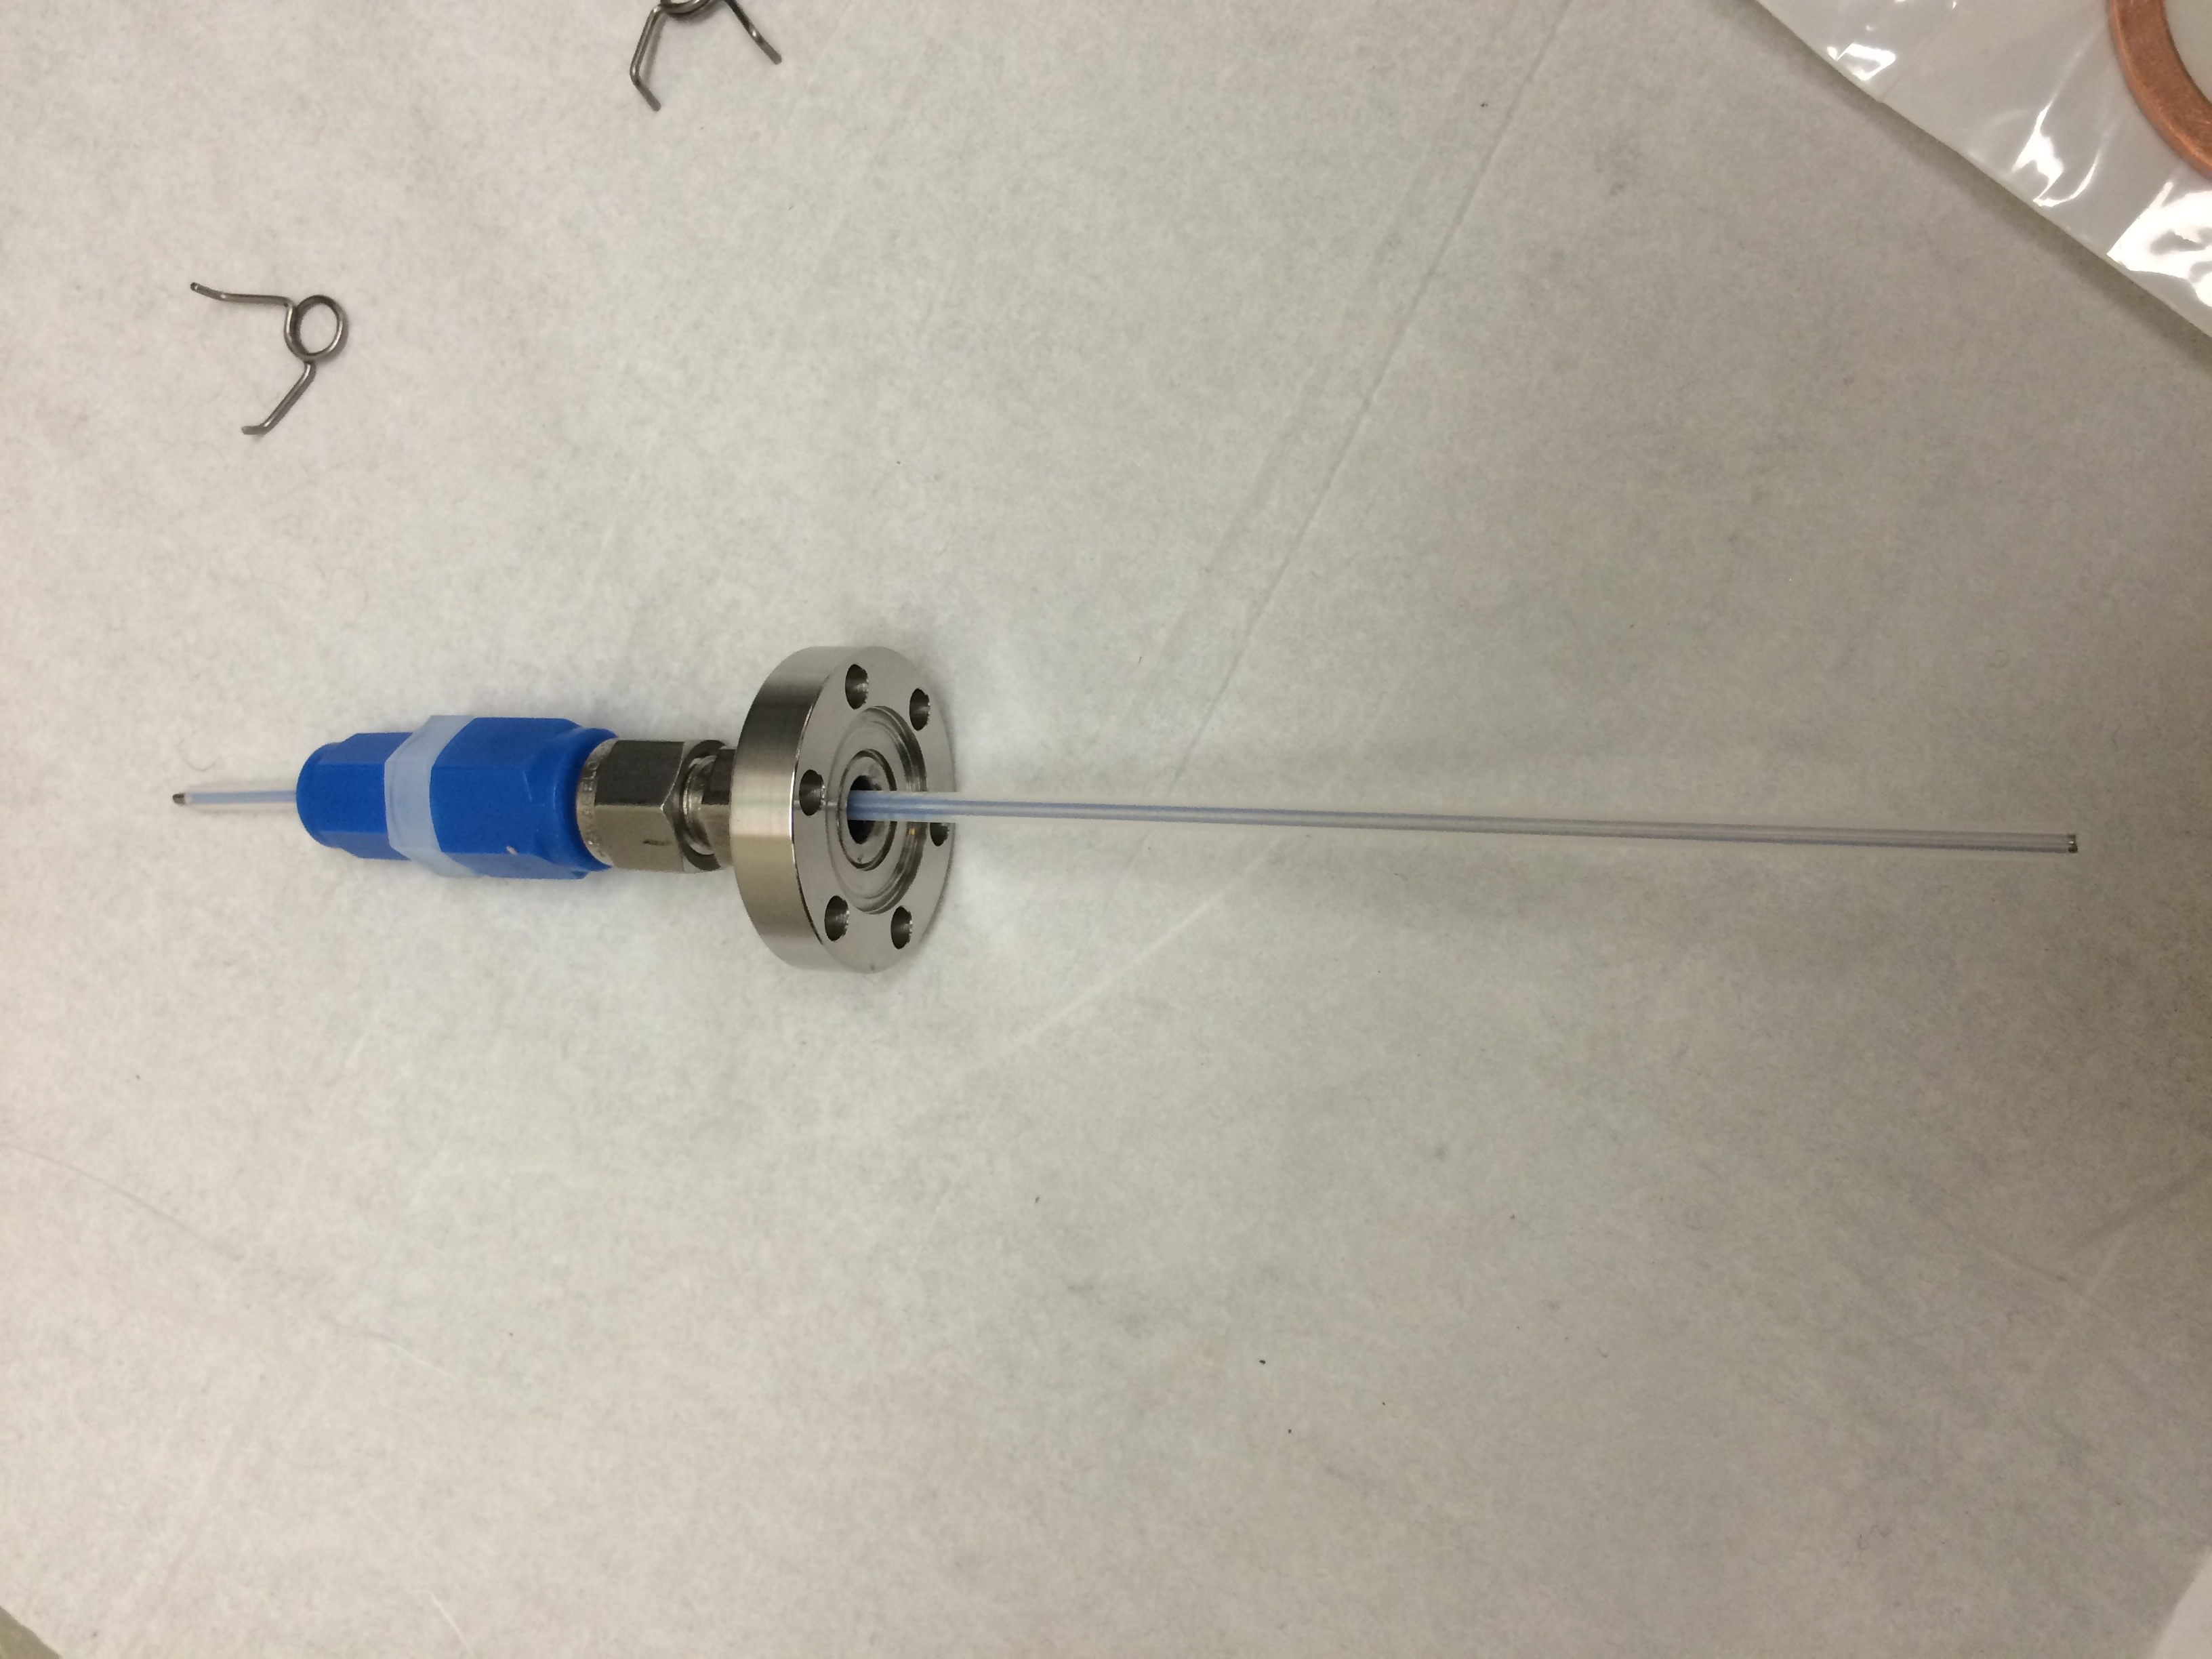
\includegraphics[width=0.3\textwidth, angle=-90]{figures/testbed/ft4_1.jpg}
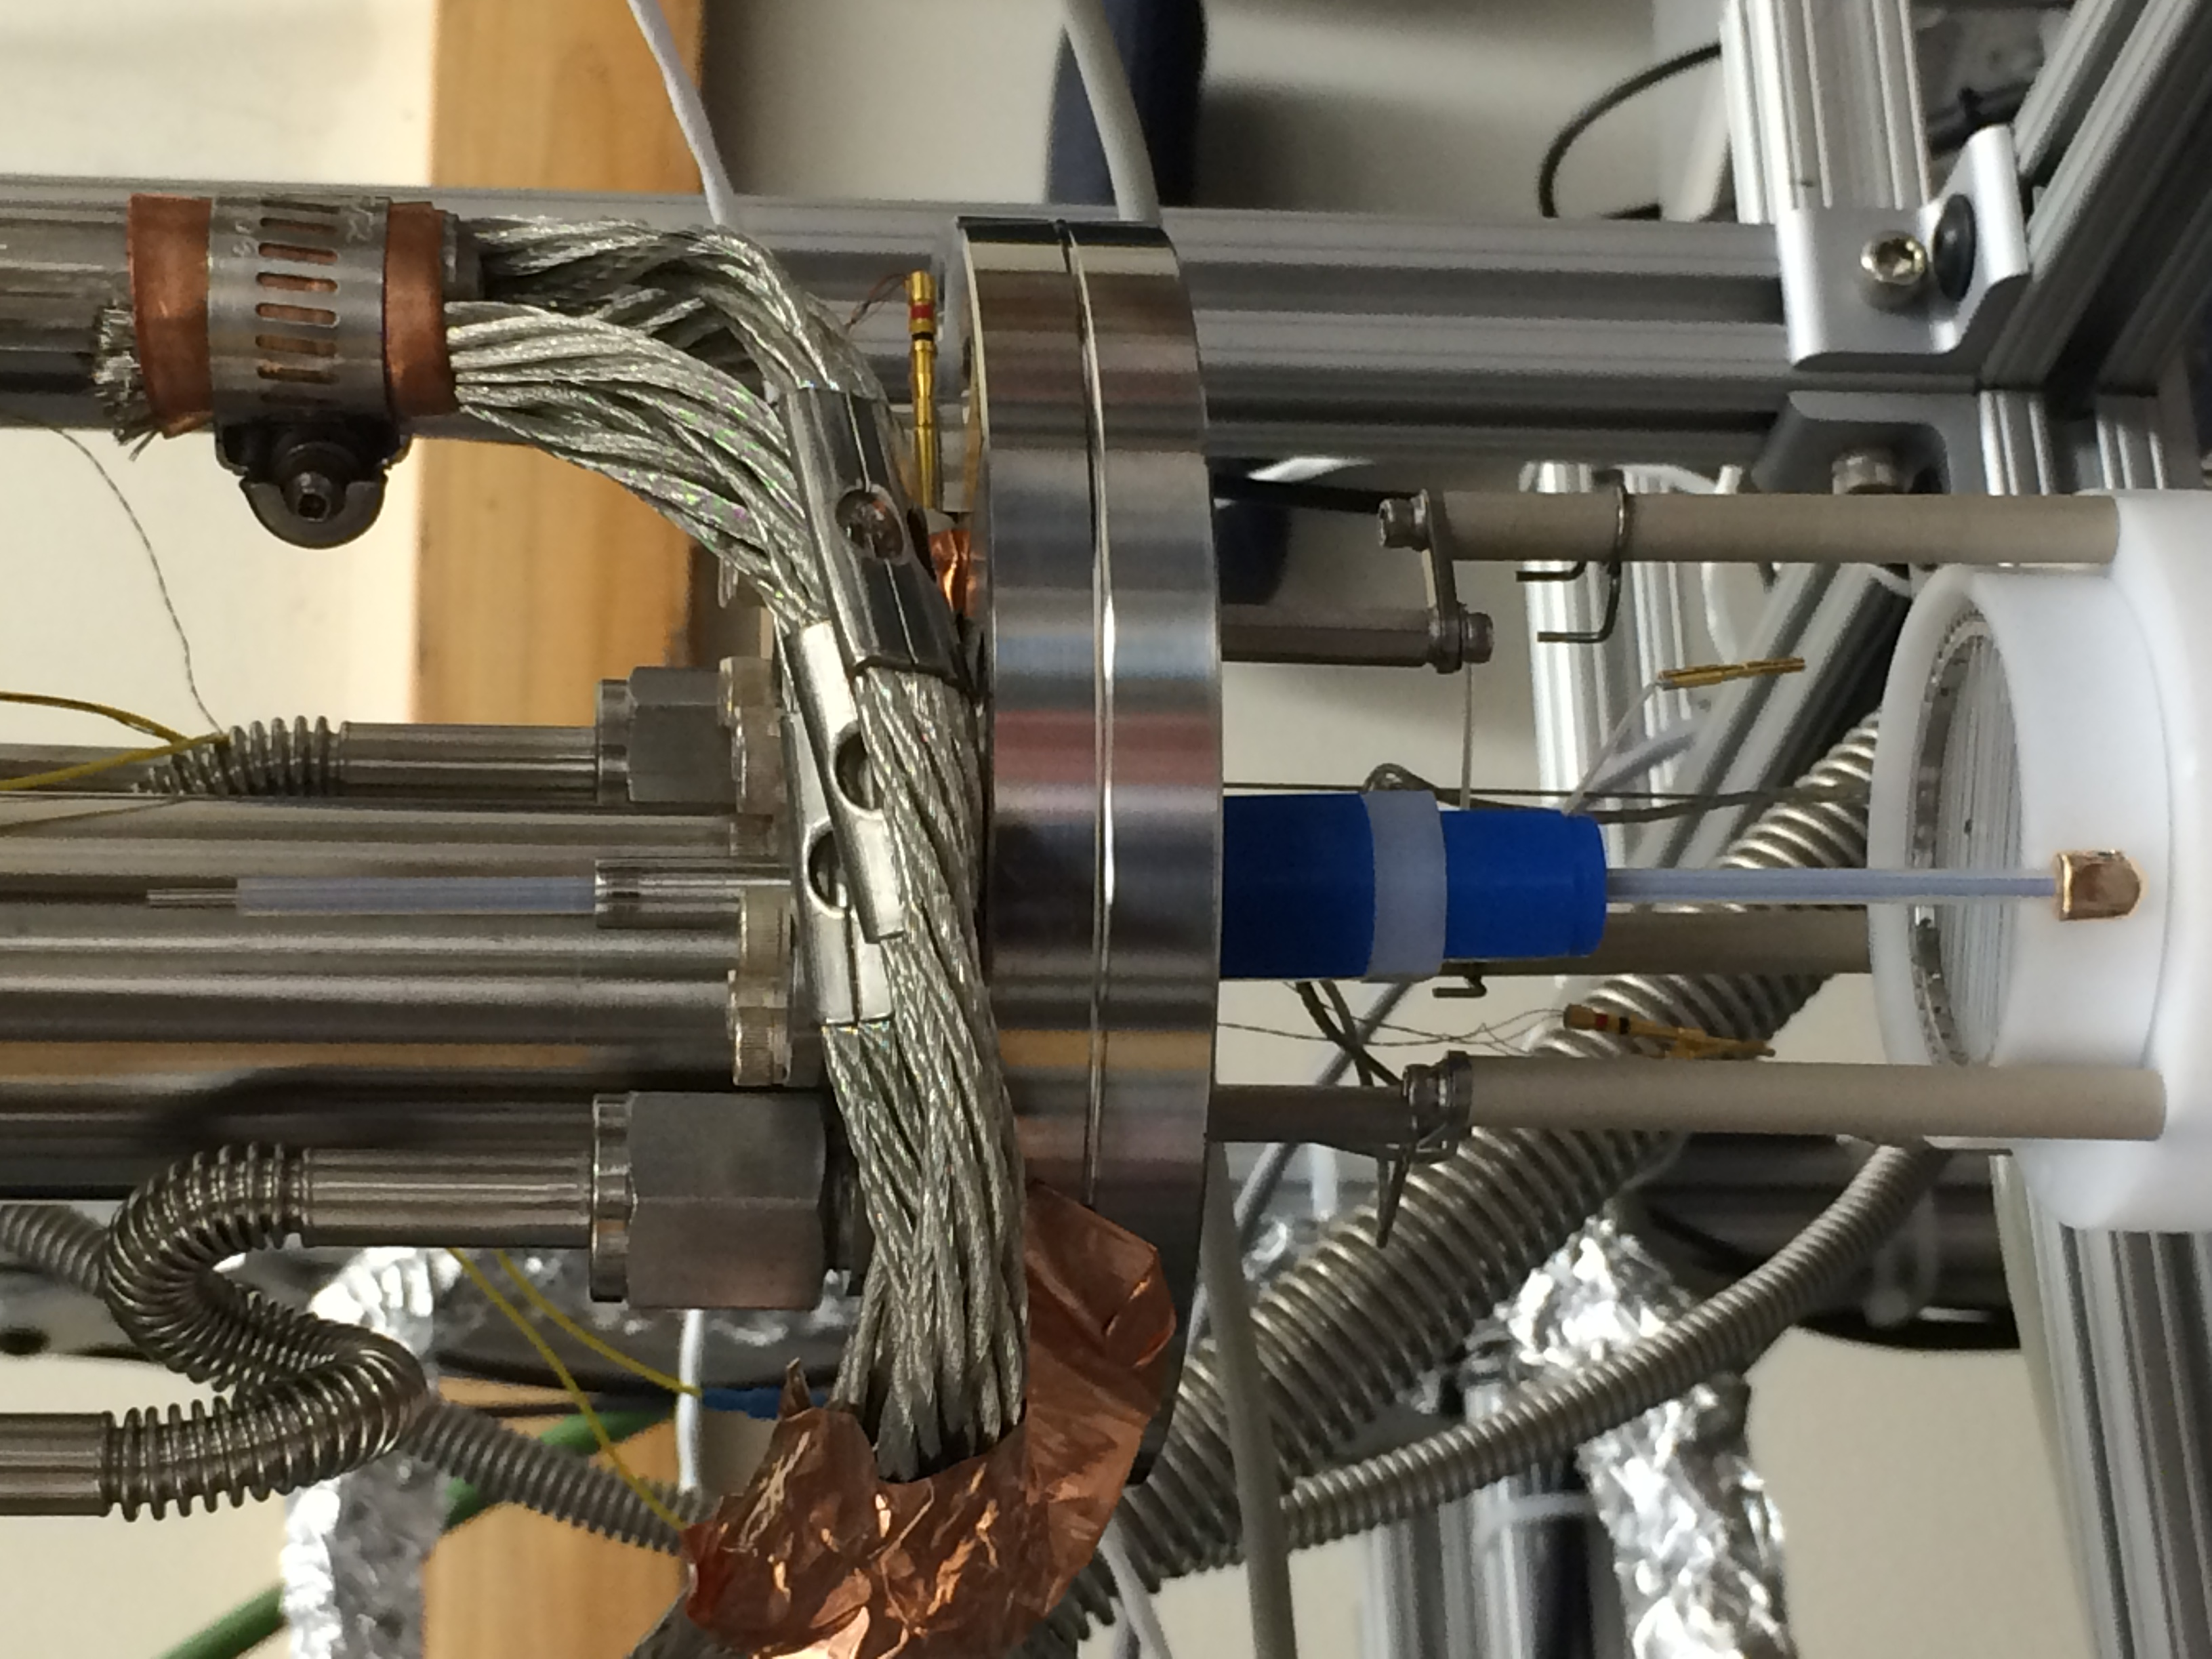
\includegraphics[width=0.3\textwidth, angle=-90]{figures/testbed/ft4_2.jpg}
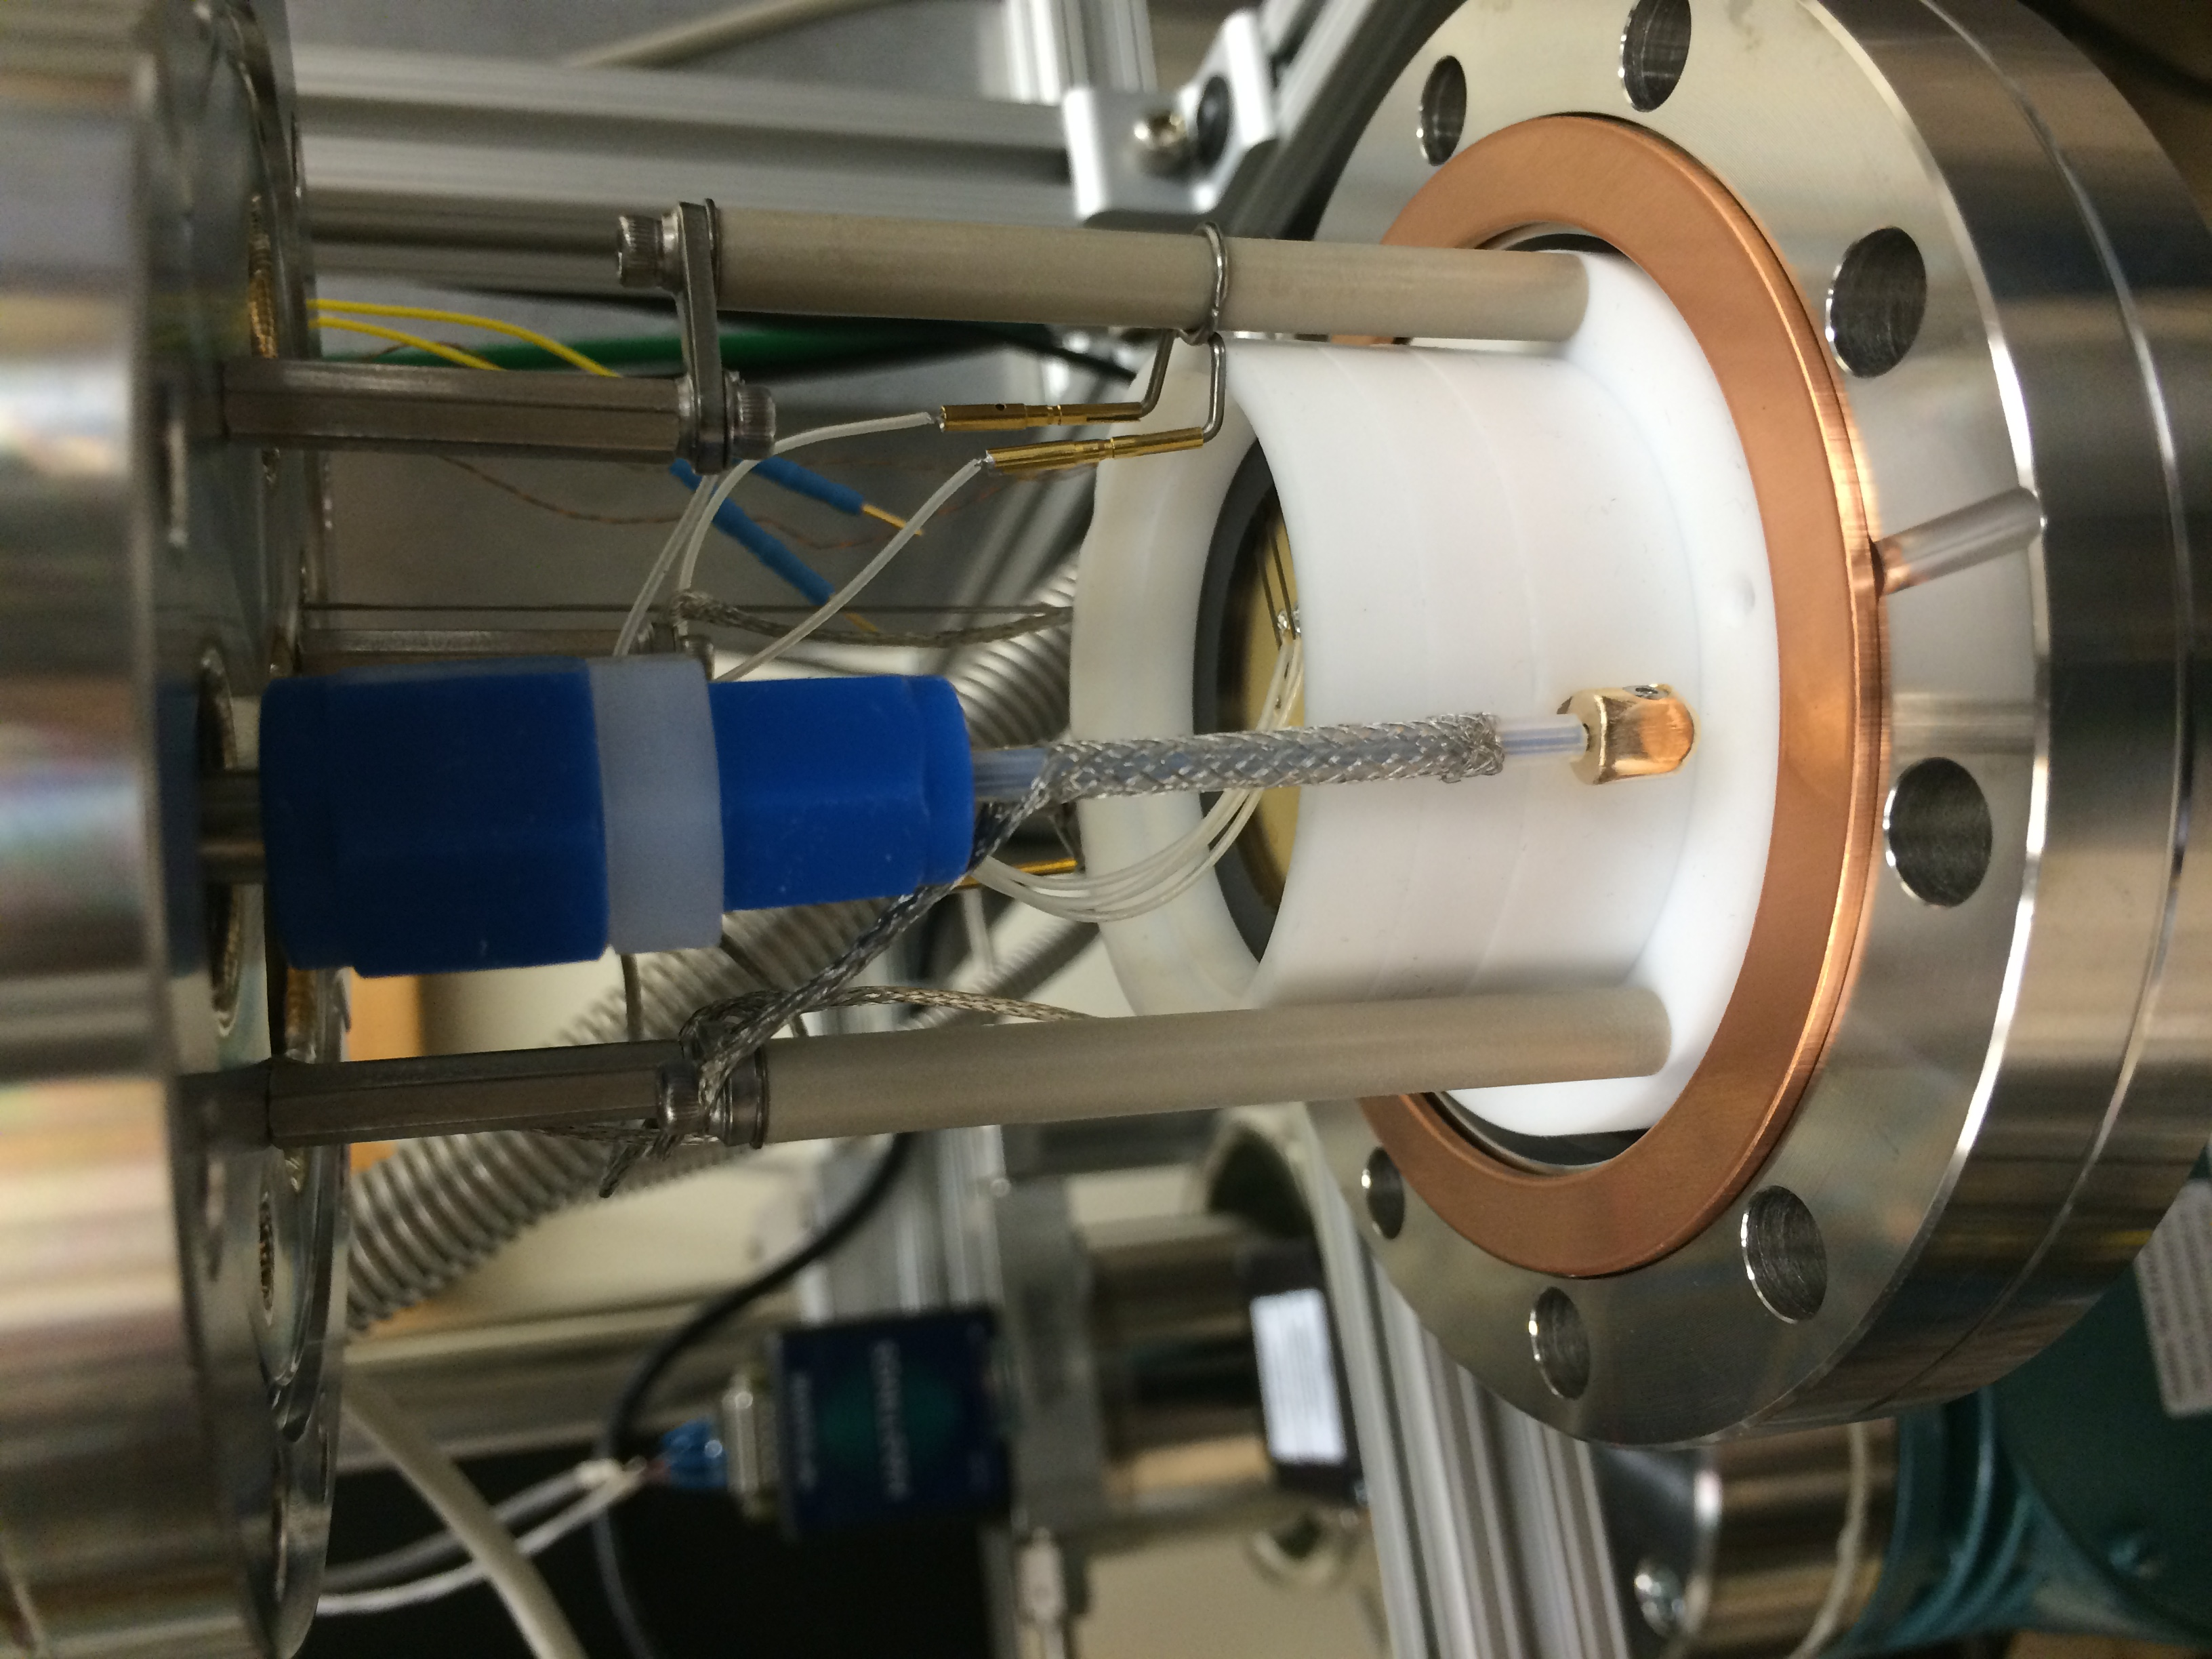
\includegraphics[width=0.3\textwidth, angle=-90]{figures/testbed/ft4_3.jpg}

\caption{First attempt at a custom feedthrough built out of Swagelock parts combined with basic materials like \acs{PTFE} and stainless steel rods. The orientation shown (left) was later inverted due to concerns of temperature stress and pressure stress on the \acs{PTFE} ferrules. The feedthrough as assembled (center) was functional, but higher voltage capability was desired. The effect of adding a grounding braid (right) was found to decrease the voltage capability instead of increasing it.  }
\label{fig:ft4}
\end{center}
\end{figure}


There are two issues with the approach of adding a grounding braid in this method: (1) the braid is not held in place tightly along the dielectric, which introduces peak fields between the dielectric and the braid (Figure~\ref{fig:will_comsol}) (2) at the braid termination, a small effective radius creates an enhanced radial field through the  dielectric and an enhanced field along the cable dielectric facing the high voltage. Peak fields can occur in unexpected places, greatly decreasing the voltage capability of a feedthrough that seems, naively, robust. The breakdown field of xenon gas depends on a variety of factors such as temperature (i.e density), purity, electrode shape, etc. Peak fields arising in gas regions in or around \ac{HV} feedthroughs are sources of unwanted light and, in the worst case, complete breakdown and eventual degradation of the feedthrough. 

\begin{figure}[htbp]
\begin{center}
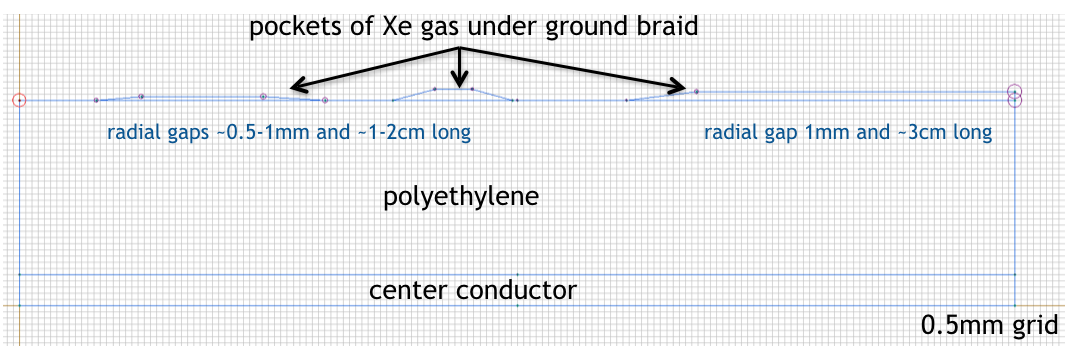
\includegraphics[width=\textwidth]{figures/testbed/will_comsol_1.png}\\
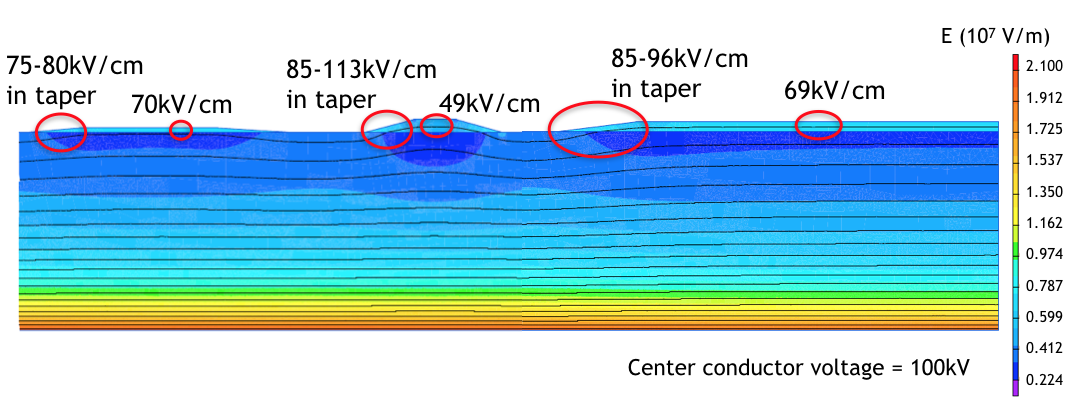
\includegraphics[width=\textwidth]{figures/testbed/will_comsol_2.png}
\caption{(top) Input to a COMSOL model simulating gaps between the grounding braid and dielectric of a high voltage feedthrough. (bottom) COMSOL output of the model, showing that peak fields arise when gaps exist between dielectric and grounding braid. Both images provided by W. Waldron.}
\label{fig:will_comsol}
\end{center}
\end{figure}

Due to the poor performance of the Swagelock \ac{PTFE} custom feedthrough (Figure~\ref{fig:ft4}) and concerns about the cold connection, another feedthrough was built out of a \ac{SS} rod with \ac{PTFE} dielectric and no shield braid (Figure~\ref{fig:ssrodft}). The rod was inserted into the \ac{PTFE} tube while warm (the tube was snug on the rod, and no temperature contraction or expansion of the \ac{PTFE} tube was done). The \ac{PTFE} ferrules formed a vacuum-tight seal on the \ac{PTFE} tube, but some epoxy at the top where the rod exits the tube is necessary (see Figure~\ref{fig:ssrodft} (top left and right)); helium leak rates during testing were around $10^{-10} - 10^{-9}$~mbar~l/s. The vacuum test was done by creating a test piece from a short piece of \acs{SS} rod and \acs{PTFE} tube; the test piece was sealed with the \acs{PTFE} ferrules with epoxy where the rod exited the \acs{PTFE} tube (no epoxy at the ferrules) and tested with a helium leak checker over the course of several hours. A pressure test was also done where the test piece was placed on a small \acs{SS} vessel which was then filled with N$_{2}$ gas until the total pressure was 3~bar. The test piece was left overnight at 3~bar of pressure and no drop in pressure was observed the next day. The total pressure was then increased to 4~bar, and left for approximately 10 hours. Again, no drop in pressure was observed. When the feedthrough was installed on the experimental vessel, more epoxy was added inside the swage nut near the ferrules for extra assurance. This feedthrough entered the inner vessel at the top of the tall \ac{CF} tower, where the connection is warm. The xenon-facing side was a copper rod bent into a U-shape which connected to the \ac{SS} conductor rod via a pin, and the other end, which was threaded, screwed into the cathode grid frame. The bare copper section was only exposed under the liquid level, and elsewhere the \ac{PTFE} dielectric helped contain the electric field and prevent breakdown to the inner vessel wall. This feedthrough had good voltage performance, and there was no sign of aging. It was decided, however, that the charge amplifiers were more susceptible to detecting transients from an unshielded feedthrough, so another feedthrough with shielding was constructed. 

%\begin{figure}[htbp]
%\begin{minipage}{0.47\textwidth}
%    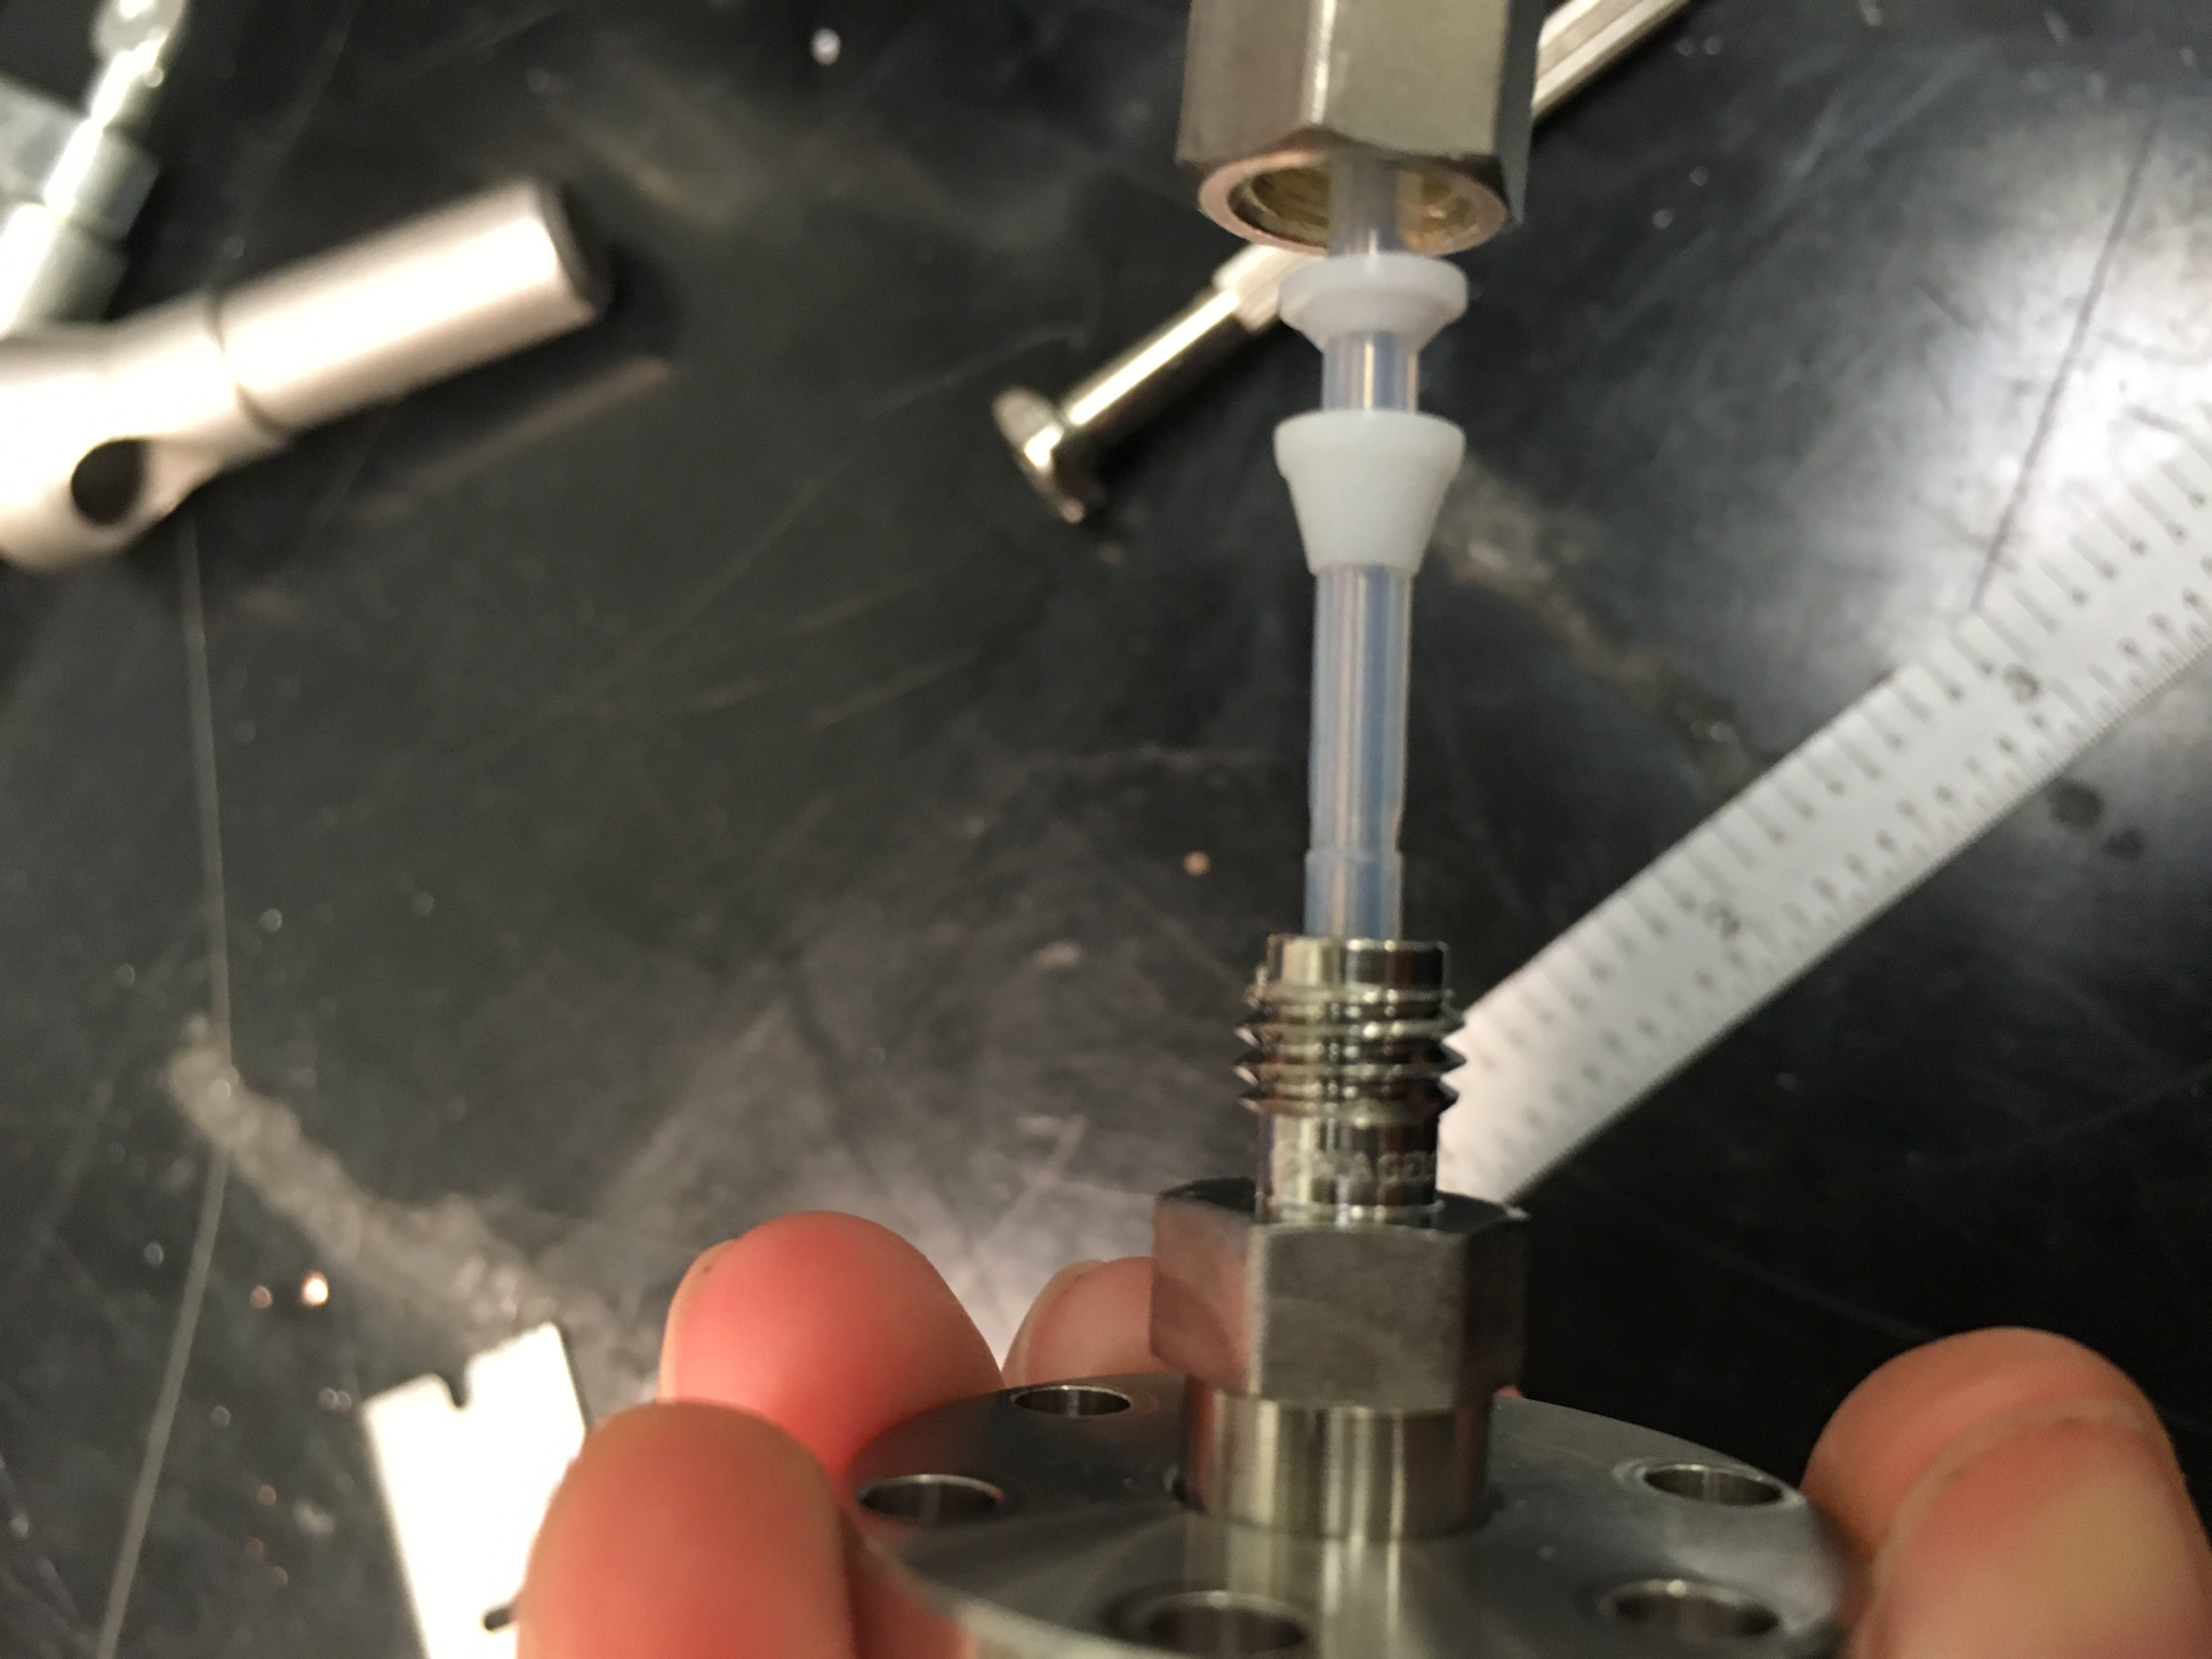
\includegraphics[width=\linewidth, angle=270]{figures/testbed/ft5_1.jpg}
 %   \end{minipage}
 %   \hspace{\fill} % note: no blank line here
 %   \begin{minipage}{0.47\textwidth}
 %   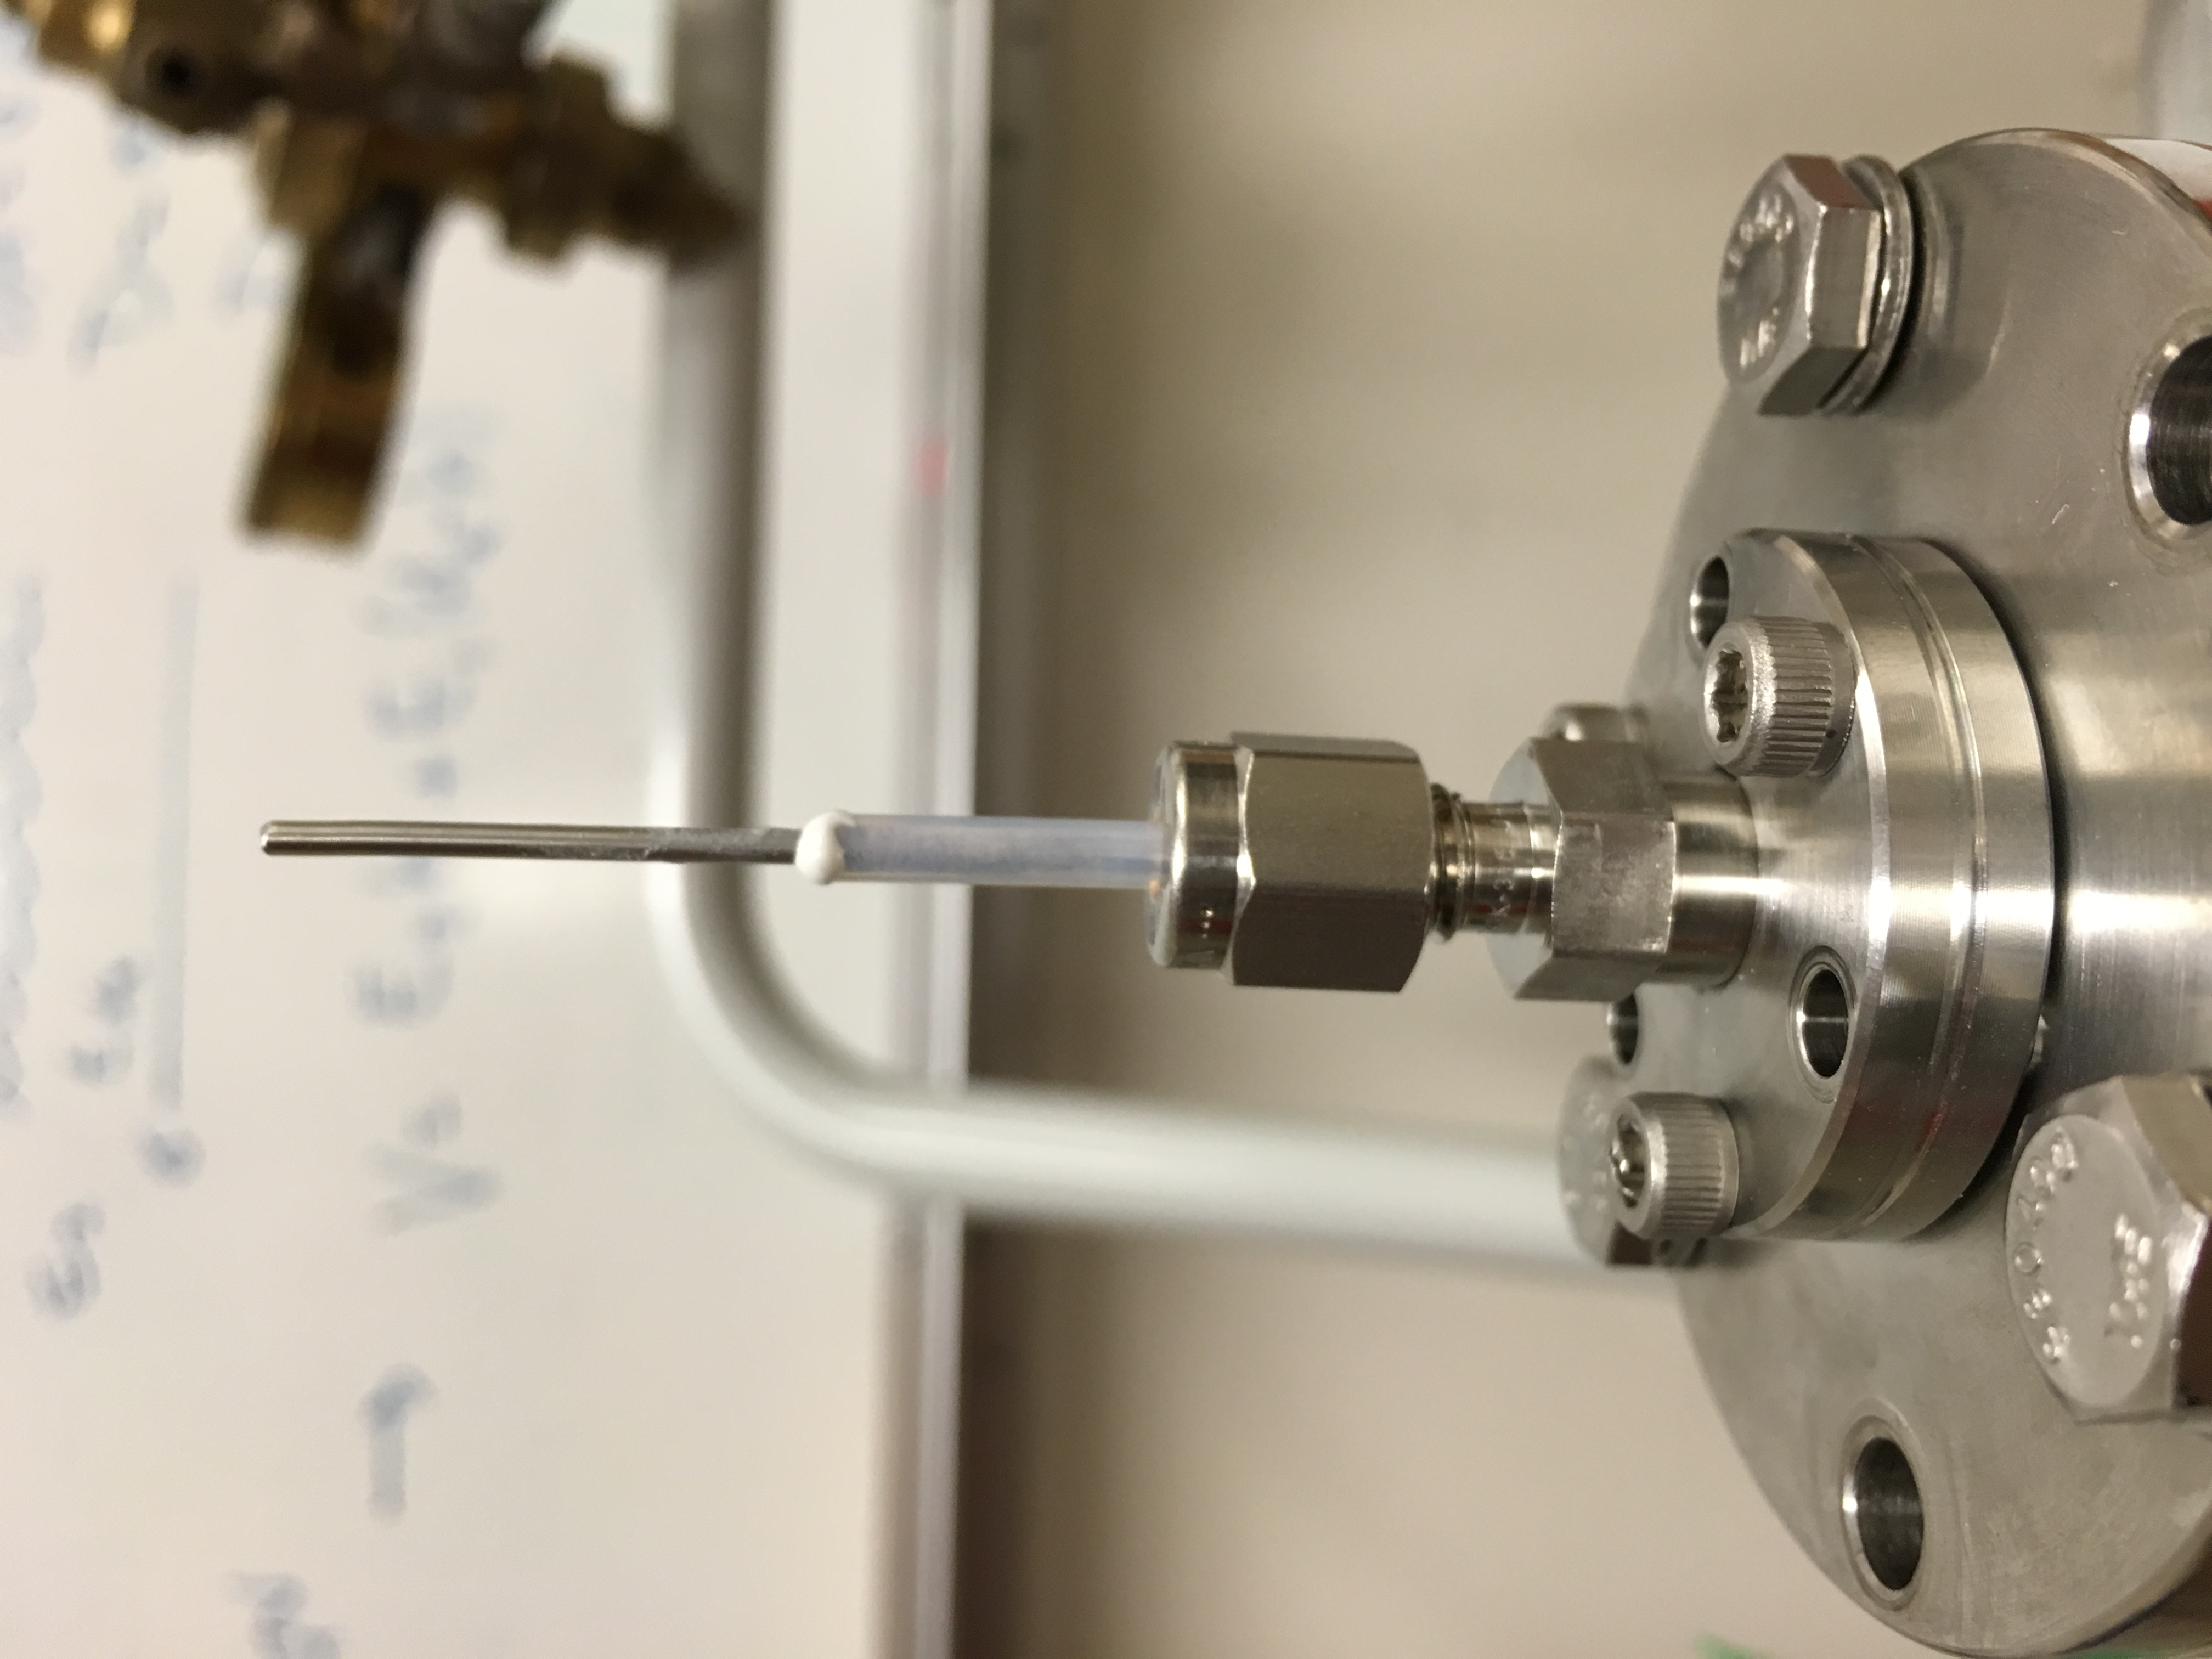
\includegraphics[width=\linewidth, angle=270]{figures/testbed/ft5_2.jpg}
 %  \end{minipage}

  %  \vspace*{1cm} % vertical separation

 %   \begin{minipage}{0.47\textwidth}
 %   \includegraphics[width=\linewidth, angle=270]{figures/testbed/ft5_3.jpg}
 %   \end{minipage}
  %  \hspace{\fill} % note: no blank line here
 %   \begin{minipage}{0.47\textwidth}
%    \includegraphics[width=\linewidth, angle=270]{figures/testbed/ft5_4.jpg}
 %   \end{minipage}
%\caption{Top: (left) Close up showing the \acs{PTFE} ferrules and notch. (right) Close up of the sealed top connection; epoxy was added to prevent leaks between the dielectric and conductor rod . Bottom: (left) %Threaded U-bend cathode connector (right) Feedthrough assembled and installed.}
 %\label{fig:ssrodft}
%\end{figure}

\begin{figure}[htbp]
\includegraphics[width=0.5\textwidth, angle=-90]{figures/testbed/ft5_1.jpg}
\includegraphics[width=0.5\textwidth, angle=-90]{figures/testbed/ft5_2.jpg}\\      
    
\includegraphics[width=0.5\textwidth, angle=-90]{figures/testbed/ft5_3.jpg}
\includegraphics[width=0.5\textwidth, angle=-90]{figures/testbed/ft5_4.jpg}  
\caption{Top: (left) Close up showing the \acs{PTFE} ferrules and notch. (right) Close-up of the sealed top connection. Although the \acs{PTFE} ferrules and some epoxy where the rod exited the \acs{PTFE} tube kept an acceptable vacuum and pressure seal, more epoxy was added during installation on the experimental vessel inside the swage nut near the ferrules. Bottom: (left) Threaded U-bend cathode connector (right) Feedthrough assembled and installed.}
 \label{fig:ssrodft}
\end{figure}


\FloatBarrier
\subsection{Final Feedthrough Design} 
The final feedthrough design is shown in Figure~\ref{fig:cableft}. The number of different materials and components used were kept to a minimum in order to avoid unnecessary high voltage triple points and complicated geometries. The feedthrough is constructed from a cable with a stranded inner \ac{SS} conductor, \ac{PTFE} dielectric, an outer \ac{SS} grounding braid, and an outer \ac{PTFE} sheath. The outer \ac{PTFE} sheath functions to keep the shielding tight against the inner dielectric, to avoid gaps where peak fields can develop. The feedthrough has a warm connection, entering the experimental vessel at the top of the \ac{CF} tower. The cable is held in place with a Swagelok connection and \ac{PTFE} ferrules. Although the feedthrough held vacuum with only the \ac{PTFE} ferrules and Swagelok connection, epoxy was placed inside the swage nut around the ferrules before tightening the nut for extra assurance in the case of high pressure. Epoxy was also applied where the inner dielectric was cut back to expose the conductor, otherwise air could travel in the space between the dielectric and the conductor into the inner vessel. Inside the \ac{CF} tower, the grounding braid was connected to ground via a screw on the underside of the \ac{CF} flange. When the cable reached the xenon experimental space, the outer sheath and shielding braid were cut back in such a way to only leave unshielded dielectric below the \ac{LXe} liquid level. The inner dielectric was cut back to expose approximately 0.5~inches of conductor, but the cable was routed through the interlocking \ac{PTFE} rings such that the point where the conductor was exposed was imbedded in \ac{PTFE}. Inside the \ac{PTFE} ring, the exposed conductor was wrapped around the wire grid. This final feedthrough design has been extremely successful, and has been in use for 2 years at the time of writing this thesis.  

The cathode feedthrough design for \ac{LZ} also uses a similar, but much more sophisticated, ``cable pass through'' design where the \ac{HV}-supplying cable goes from air into xenon space without being terminated at the xenon vessel, e.g. termination in a connector, which then connects to a different cable on the inside of the vessel. The \ac{LZ} technical design report shows the scheme \cite{LZTDR}.


%\begin{minipage}{0.32\textwidth}
  %  \includegraphics[width=\linewidth, angle=270]{figures/testbed/ft6_4.jpg}
    %\end{minipage}
 %   \hspace{\fill} % note: no blank line here
  %  \begin{minipage}{0.32\textwidth}
  %  \includegraphics[width=\linewidth, angle=270]{figures/testbed/ft6_5.jpg}
 %   \end{minipage}
  %      \hspace{\fill} % note: no blank line here
   % \begin{minipage}{0.33\textwidth}
   % \includegraphics[width=\linewidth, angle=270]{figures/testbed/ft6_6.jpg}
   % \end{minipage}

   % \vspace*{1cm} % vertical separation

%    \begin{minipage}{0.32\textwidth}
 %   \includegraphics[width=\linewidth, angle=270]{figures/testbed/ft6_1.jpg}
 %   \end{minipage}
 %   \hspace{\fill} % note: no blank line here
  %  \begin{minipage}{0.32\textwidth}
  %  \includegraphics[width=\linewidth, angle=270]{figures/testbed/ft6_2.jpg}
  %  \end{minipage}
 %       \hspace{\fill} % note: no blank line here
  %  \begin{minipage}{0.32\textwidth}
  %  \includegraphics[width=\linewidth, angle=270]{figures/testbed/ft6_3.jpg}
  %  \end{minipage}



\begin{figure}[htbp]
\includegraphics[width=0.33\textwidth, angle=-90]{figures/testbed/ft6_4.jpg}
\includegraphics[width=0.33\textwidth, angle=-90]{figures/testbed/ft6_5.jpg}  
\includegraphics[width=0.33\textwidth, angle=-90]{figures/testbed/ft6_6.jpg}\\      
    
\includegraphics[width=0.33\textwidth, angle=-90]{figures/testbed/ft6_1.jpg}
\includegraphics[width=0.33\textwidth, angle=-90]{figures/testbed/ft6_2.jpg}  
\includegraphics[width=0.33\textwidth, angle=-90]{figures/testbed/ft6_3.jpg}
\caption{Top: (left) Sealed top connection with liberal epoxy use. A male Bendix pin was soldered to the cable conductor. (middle) \acs{SHV} connector with female Bendix to mate with feedthrough (right) Grounded safety housing with \acs{SHV} connector. Bottom: (left) Ends of the feedthrough were held in the Teflon stack. (middle) Close up showing cable conductor, \acs{PTFE} dielectric, and grounding sheath pulled back. The calipers are measuring the length of exposed conductor. (right) Grounding scheme for feedthrough cables at the top of the \acs{CF} tower.}
 \label{fig:cableft}
\end{figure}

\FloatBarrier
\section{Electric Fields in Test Bed}
Both peak fields, which occur on the grid wires, and fields at the liquid-gas boundary are important to understand. Peak fields are often at a ``weak link'' in the voltage chain where breakdown is most likely to occur. The field in the liquid near the gas boundary extracts electrons, making it important for \ac{TPC} function. The electric field changes as a function of liquid height, and can be calculated analytically following the McDonald lecture notes \cite{McDonald2003}. A COMSOL model with the test bed geometry and materials was also developed by E. Mizrachi. The COMSOL model and the analytic calculation were found to agree. Figure~\ref{fig:fields_on_wires} provides a summary of the electric fields on the grids wires for a case where there is only a cathode and anode, separated by 5~cm. The color scale on the COMSOL is misleading: the peak fields, which occur on the cathode wires, are $\sim$130~kV/cm, which appears the same color as 20~kV/cm.

\begin{figure}[htbp]
\begin{center}
\includegraphics[width=\halffig]{figures/testbed/COMSOL.png}
\includegraphics[width=\halffig]{figures/testbed/FieldsOnWires_withCOMSOL.png}
\caption{(left) COMSOL model with specific cathode voltage and liquid level. The peak fields of $\sim$130~kV/cm occur on the wires, and the gas fields are $\sim$20~kV/cm. These two values are both dark red on the color scale, which can be misleading. (right) Analytic calculation following the McDonald notes \cite{McDonald2003}, which shows how the peak fields vary with change in liquid level and cathode voltage. The voltages in the legend refer to the cathode voltage; the anode is held at ground.}
\label{fig:fields_on_wires}
\end{center}
\end{figure}

The COMSOL model shows that the fields in the liquid and gas do not vary very much with position, once there is sufficient distance from the wires. The fields do, however, vary with liquid level. Figure~\ref{fig:fields_in_liquid_and_gas} shows how the liquid and gas electric fields vary with liquid level and cathode voltage; the \ac{TPC} configuration ``extraction region only'' with cathode and anode separated by 0.5~cm. The calculation is straightforward: the \ac{TPC} is a essentially a capacitor with a dielectric. Cathode and anode provide boundary conditions on the voltage, and continuity of the derivatives at the liquid-gas boundary is the remaining boundary condition to solve Poisson's equation.


\begin{figure}[htbp]
\begin{center}
\includegraphics[width=\textwidth]{figures/testbed/fields_in_xaber.png}
\caption{Ranges for the electric fields in gas and liquid for different cathode voltages and liquid levels.}
\label{fig:fields_in_liquid_and_gas}
\end{center}
\end{figure}


%*****************************************
%*****************************************
%*****************************************
%*****************************************
%*****************************************
